\documentclass[a4paper,twoside,12pt]{book}



\usepackage[printonlyused,footnote]{acronym}
\usepackage{amsmath}
\usepackage{amssymb}
\usepackage{amsthm}
\usepackage[title]{appendix}
\usepackage[style=iso-numeric, 
    backend=biber, 
    language=czech
    ]{biblatex}
\usepackage[font=small,
    labelfont=bf]{caption}
\usepackage{csquotes}
\usepackage[resetfonts]{cmap}
\usepackage{emptypage}
\usepackage{fancyhdr}
\usepackage{float}
\usepackage[T1]{fontenc}            % font encoding
\usepackage{gensymb}
\usepackage[a4paper,
    hmarginratio=3:2
]{geometry}                         % geometry of page, margins etc.
\usepackage{graphicx}
\usepackage[hidelinks,
    unicode]{hyperref}              % clickable links
\usepackage{import}
\usepackage{indentfirst}
\usepackage[utf8]{inputenc}         % UTF-8 character set
\usepackage{listings}
\usepackage{lmodern}
\usepackage{makecell}               % for tables
\usepackage[version=3]{mhchem}
\usepackage{paralist}
\usepackage{pdfpages}
\usepackage{tabularx} 
\usepackage[nottoc]{tocbibind}      % citations
\usepackage{tocloft}
\usepackage{upgreek}
\usepackage{xargs}
%%% Specification of all necessary stuff %%%
% ========================================


% Specification of the author and consultants
\newcommand{\autor}{Thesis Author}   % vyplňte své jméno a příjmení (s akademickým titulem, máte-li jej)
\newcommand{\woman}{} % pokud jste ŽENA, ZMĚŇTE na: ...{\woman}{a} (je to do Prohlášení)

\newcommand{\vedouci}{title. Great Supervisor} % vyplňte jméno a příjmení vedoucího práce, včetně titulů, např.: Doc. Ing. Ivo Malý, Ph.D.
\newcommand{\pracovisteVed}{Awesome and Rich company from Supervisor} % ZMĚŇTE, pokud vedoucí Vaší práce není z KSI
\newcommand{\konzultant}{title. Talkative Consultant} % POKUD MÁTE určeného konzultanta, NAPIŠTE jeho jméno a příjmení
\newcommand{\pracovisteKonz}{Very consultive Group} % POKUD MÁTE konzultanta, NAPIŠTE jeho pracoviště
\newcommand{\konzultantt}{title. Awesome SecondOne} % POKUD MÁTE určeného konzultanta, NAPIŠTE jeho jméno a příjmení
\newcommand{\pracovisteKonzt}{The second Group} % POKUD MÁTE konzultanta, NAPIŠTE jeho pracoviště

% Specification of thesis -- copy and paste from your task list
\newcommand{\nazevcz}{Název česky}
\newcommand{\nazeven}{Název anglicky}
\newcommand{\rok}{2020}  % rok odevzdání práce (jen rok odevzdání, nikoli celý akademický rok!)
\newcommand{\skola}{School name (see commands.tex for acronyms)}
\newcommand{\fakulta}{Faculty name (see commands.tex for acronyms)}
\newcommand{\katedra}{Department name (see commands.tex for acronyms)}
\newcommand{\kde}{Praze} % studenti z Děčína ZMĚNÍ na: "Děčíně" (doplní se k "prohlášení")
\newcommand{\program}{Aplikace přírodních věd} % změňte, pokud máte jiný stud. program
\newcommand{\obor}{Jaderné inženýrství} % změňte, pokud máte jiný obor

%% LANGUAGE SETTINGS
% Uncomment exactly one block

%==================
%% CZECH
\usepackage[czech]{babel} % česky psaná práce, typografická pravidla. Překládejte pomocí "latex.exe" nebo "pdflatex.exe"

% Uncomment exactly one 
\newcommand{\druh}{Bakalářská práce} 
%\newcommand{\druh}{Výzkumný úkol} 
%\newcommand{\druh}{Diplomová práce}
%==================

%==================
%% SLOVAK
% \usepackage[slovak]{babel} 
%==================


%==================
%% ENGLISH
% \usepackage[english]{babel}

% Uncomment exactly one 
%\newcommand{\druh}{Bachelor thesis} 
%\newcommand{\druh}{Research project} 
%\newcommand{\druh}{Master thesis}
%==================



% Insert scan of your task -- put it in "img" folder -- 2 separate PDFs recommended
\newcommand{\skenZadaniPredni}{specimen1.pdf}
\newcommand{\skenZadaniZadni}{specimen2.pdf}

% Keywords in zde NAPIŠTE česky max. 5 klíčových slov AND translate them into english
\newcommand{\klicova}{slovo1, slovo2, slovo3}  
\newcommand{\keyword}{keyword1, keyword2, keyword3}
\newcommand{\abstrCZ}{% zde NAPIŠTE abstrakt v češtině (cca 7 vět, min. 80 slov)
Tato práce se zabývá psaním závěrečných prací.
}
\newcommand{\abstrEN}{% zde NAPIŠTE abstrakt v angličtině
The thesis deals with the issue of thesis writing. 
}
\newcommand{\prohlaseni}{% text prohlášení můžete mírně upravit
Prohlašuji, že jsem svou bakalářskou práci vypracoval\woman{} samostatně a použil\woman{} jsem pouze podklady (literaturu, projekty, SW atd.) uvedené v přiloženém seznamu.
} 
\newcommand{\podekovani}{%Podekovani se doporucuje neprehanet
 Děkuji Ing. Eleonoře Krtečkové, Ph.D. za vedení mé bakalářské práce a za podnětné návrhy, které ji obohatily.
% NEBO:
% Děkuji vedoucímu práce doc. Pafnutijovi Snědldítětikaši, Ph.D. za neocenitelné rady a pomoc při tvorbě bakalářské práce.
}

% Page style -- uncomment exactly one
% 
% Style 1 -- fancy -- nice looking, but unfortunatelly, not debugged yet :(
% \pagestyle{fancy}
% \fancyfoot{}
% \fancyhead[RO,LE]{\thepage}
% \fancyhead[RE]{\nouppercase{\leftmark}}
% \fancyhead[LO]{\nouppercase{\rightmark}}

% Style 2 -- plain
\pagestyle{plain}      % stránky číslované dole uprostřed


% Page numbering
\pagenumbering{arabic} % číslování stránek arabskými číslicemi

% Depth of table of contents (ToC) (2 is RECOMMENDED, other are believed to be confusing and poorly arranged!
% 0 = only parts and chapters are included in ToC
% 1 = parts, chapters, sections
% 2 = parts, chapters, sections, subsections
% 3 = parts, chapters, sections, subsections, subsubsections
\setcounter{tocdepth}{2}


% Margins 
\topmargin=-10mm      % horní okraj trochu menší
\textwidth=150mm      % šířka textu na stránce
\textheight=250mm     % "výška" textu na stránce

% Intendation
\parindent=0pt % odsazení 1. řádku odstavce
\parskip=7pt   % mezera mezi odstavci

% Font size
\renewcommand\cftchapfont{\small\bfseries}
\renewcommand\cftsecfont{\footnotesize}
\renewcommand\cftsubsecfont{\footnotesize}

\renewcommand\cftchappagefont{\small\bfseries}
\renewcommand\cftsecpagefont{\footnotesize}
\renewcommand\cftsubsecpagefont{\footnotesize}

% Spacing
\frenchspacing % za větou bude mezislovní mezera (v anglických textech je mezera za větou delší)
\widowpenalty=1000 % "síla" zákazu vdov (= jeden řádek ze začátku odstavce na konci stránky)
\clubpenalty=1000 % "síla" zákazu sirotků (= jeden řádek/slovo z konce odstavce samostatně na začátku stránky)
\brokenpenalty=1000 % "síla" zákazu zlomu stránky za řádkem, který má na konci rozdělené slovo

% Aliases

%% Font
\newcommand{\bv}{\mathbf} % bold math
\newcommand{\tb}{\textbf} % bold font
\newcommand{\ti}{\textit} % itallic font

%% Paralist environments
%%% shorter compactenum
\newcommandx{\cen}[1]{
    \begin{compactenum}
        #1
    \end{compactenum}
}
%%% shorter compactitem
\newcommandx{\cit}[1]{
    \begin{compactitem}
        #1
    \end{compactitem}
}

% Commands

%% Graphics

%%% Single figure
    \newcommandx{\pic}[5][4=0.8,5=H]{%
        \begin{figure}[#5]
            \centering
            \includegraphics[width=#4\textwidth]{./img/#1}
            \caption[#2]{#3}
            \label{#1}
        \end{figure}
    }

    %%% Two pictures side-by-side
    \newcommandx{\dpic}[9][7=0.49,8=0.98,9=H]{%
        \begin{figure}[#9]
            \centering
            \begin{minipage}{#7\textwidth}
                \centering
                \includegraphics[width=#8\textwidth]{img/#1} % first figure itself
                \caption[#3]{#4}
                \label{#1}
            \end{minipage}\hfill
            \begin{minipage}{#7\textwidth}
                \centering
                \includegraphics[width=#8\textwidth]{img/#2} % second figure itself
                \caption[#5]{#6}
                \label{#2}
            \end{minipage}
        \end{figure}
    }

    %%% Three figures side-by-side... Not really sure, whether it looks good
    \newcommandx{\tpic}[9]{%
        \begin{figure}[H]
            \centering
            \begin{minipage}{0.3\textwidth}
                \centering
                \includegraphics[width=0.95\textwidth]{img/#1} % first figure itself
                \caption[#2]{#3}
                \label{#1}
            \end{minipage}\hfill
            \begin{minipage}{0.3\textwidth}
                \centering
                \includegraphics[width=0.95\textwidth]{img/#4} % second figure itself
                \caption[#5]{#6}
                \label{#4}
            \end{minipage}\hfill
            \begin{minipage}{0.3\textwidth}
                \centering
                \includegraphics[width=0.95\textwidth]{img/#7} % second figure itself
                \caption[#8]{#9}
                \label{#7}
            \end{minipage}
        \end{figure}
    }

%% Better footnotes above punctuation
\newcommand{\footnotei}[2]{%
    \mbox{%
        \setbox0\hbox{#1}%
        \copy0%
        \hspace{-\wd0}}%
    \footnote{#2}%
}

%% Equations
\newcommandx{\eq}[1]{
    \begin{equation}
        #1
    \end{equation}
}
\newcommandx{\eqa}[1]{
    \begin{align}
        #1
    \end{align}
}

%% Units
\newcommand{\jdt}[1]{
    $\mathrm{#1}$
}

\newcommand{\jde}[1]{
    \mathrm{#1}
}

%% Derivative faster
\newcommand{\der}[2]{
    \frac{\mathrm{d} #1}{\mathrm{d} #2}
}

%% N-th derivative faster
\newcommand{\nder}[3]{
    \frac{\mathrm{d}^{#3} #1}{\mathrm{d} {#2}^{#3}}
}

%% Partial derivative faster
\newcommand{\pder}[2]{
    \frac{\partial #1}{\partial #2}
}

%% N-th partial derivative faster
\newcommand{\npder}[3]{
    \frac{\partial^{#3} #1}{\partial {#2}^{#3}}
}

%% Auto-sized brackets
\renewcommand{\(}{
    \left(
}
\renewcommand{\)}{
    \right)
}

\renewcommand{\[}{
\left[
}
\renewcommand{\]}{
    \right]
}

% \_ for non-itallic sub indices
\let\underscore\_                                           % underscore sign
\let\xor\^                                                  % xor sign
\renewcommand\_[2][1]{\ifmmode _{\textnormal{\scalebox{#1}{#2}}}\else\underscore#2\fi} %roman subscript
\renewcommand\^[2][1]{\ifmmode ^{\textnormal{\scalebox{#1}{#2}}}\else\xor#2\fi} %roman superscript
\def\smallind{0.8}

%% Math aliases
\newcommand{\mdef}[3]{
	\begin{define}[#1]
		\label{mdef:#2}
		#3
	\end{define}
}

\newcommand{\mtheor}[3]{
	\begin{theorem}[#1]
		\label{mtheor:#2}
		#3
	\end{theorem}
}

\newcommand{\mlemma}[3]{
	\begin{lemma}[#1]
		\label{mlemma:#2}
		#3
	\end{lemma}
}

\newcommand{\mcomm}[3]{
	\begin{comment}[#1]
		\label{mcomm:#2}
		#3
	\end{comment}
}

\newcommand{\mex}[2]{
	\begin{example}
		\label{mex:#1}
		#2
	\end{example}
}


\begin{document}

\frontmatter

\thispagestyle{empty}

\begin{center}
	{\LARGE
		\cvut\par
		\fjfi
	}
    \vspace{10mm}

    \begin{tabular}{c}
		\tb{\kjr} \\[3pt]   
		\tb{Obor: \obor}\\
    \end{tabular}

   \vspace{10mm} \logoCVUT \vspace{15mm} 

   {\huge \tb{\nazevcz}\par}
   \vspace{5mm}   
   {\huge \tb{\nazeven}\par}
   
   \vspace{15mm}
   {\Large \MakeUppercase{\druh}}

   \vfill
   {\large
    \begin{tabular}{ll}
    Vypracoval: & \autor\\
    Vedoucí práce: & \vedouci\\
    Rok: & \rok
    \end{tabular}
   }
\end{center}

\clearpage{\pagestyle{empty}\cleardoublepage} % prázdná stránka za tou "titulní", bez čísla

%%%%%%%%%%%% ZADÁNÍ PRÁCE %%%%%%%%%%%%
% Zadání (podepsané děkanem!) musíte NASKENOVAT. Ideálně jako 2stránkové PDF (soubor "zadani_cele.pdf"). 
% Před svázáním to v jednom výtisku VYMĚNÍTE ZA ORIGINÁLNÍ ZADÁNÍ (podepsané děkanem fakulty)!
\newpage  % SEM NESAHEJTE!
\thispagestyle{empty} % SEM NESAHEJTE!

%% zde podle toho, jak jste zadání naskenovali, VYBERTE variantu A, B nebo C:
%
% --- varianta A: zadání naskenované jako 2stránkové PDF:

\includepdf[pages={1}]{img/bp-rzehulka-zad1.pdf} % NAHRAĎTE správným souborem!
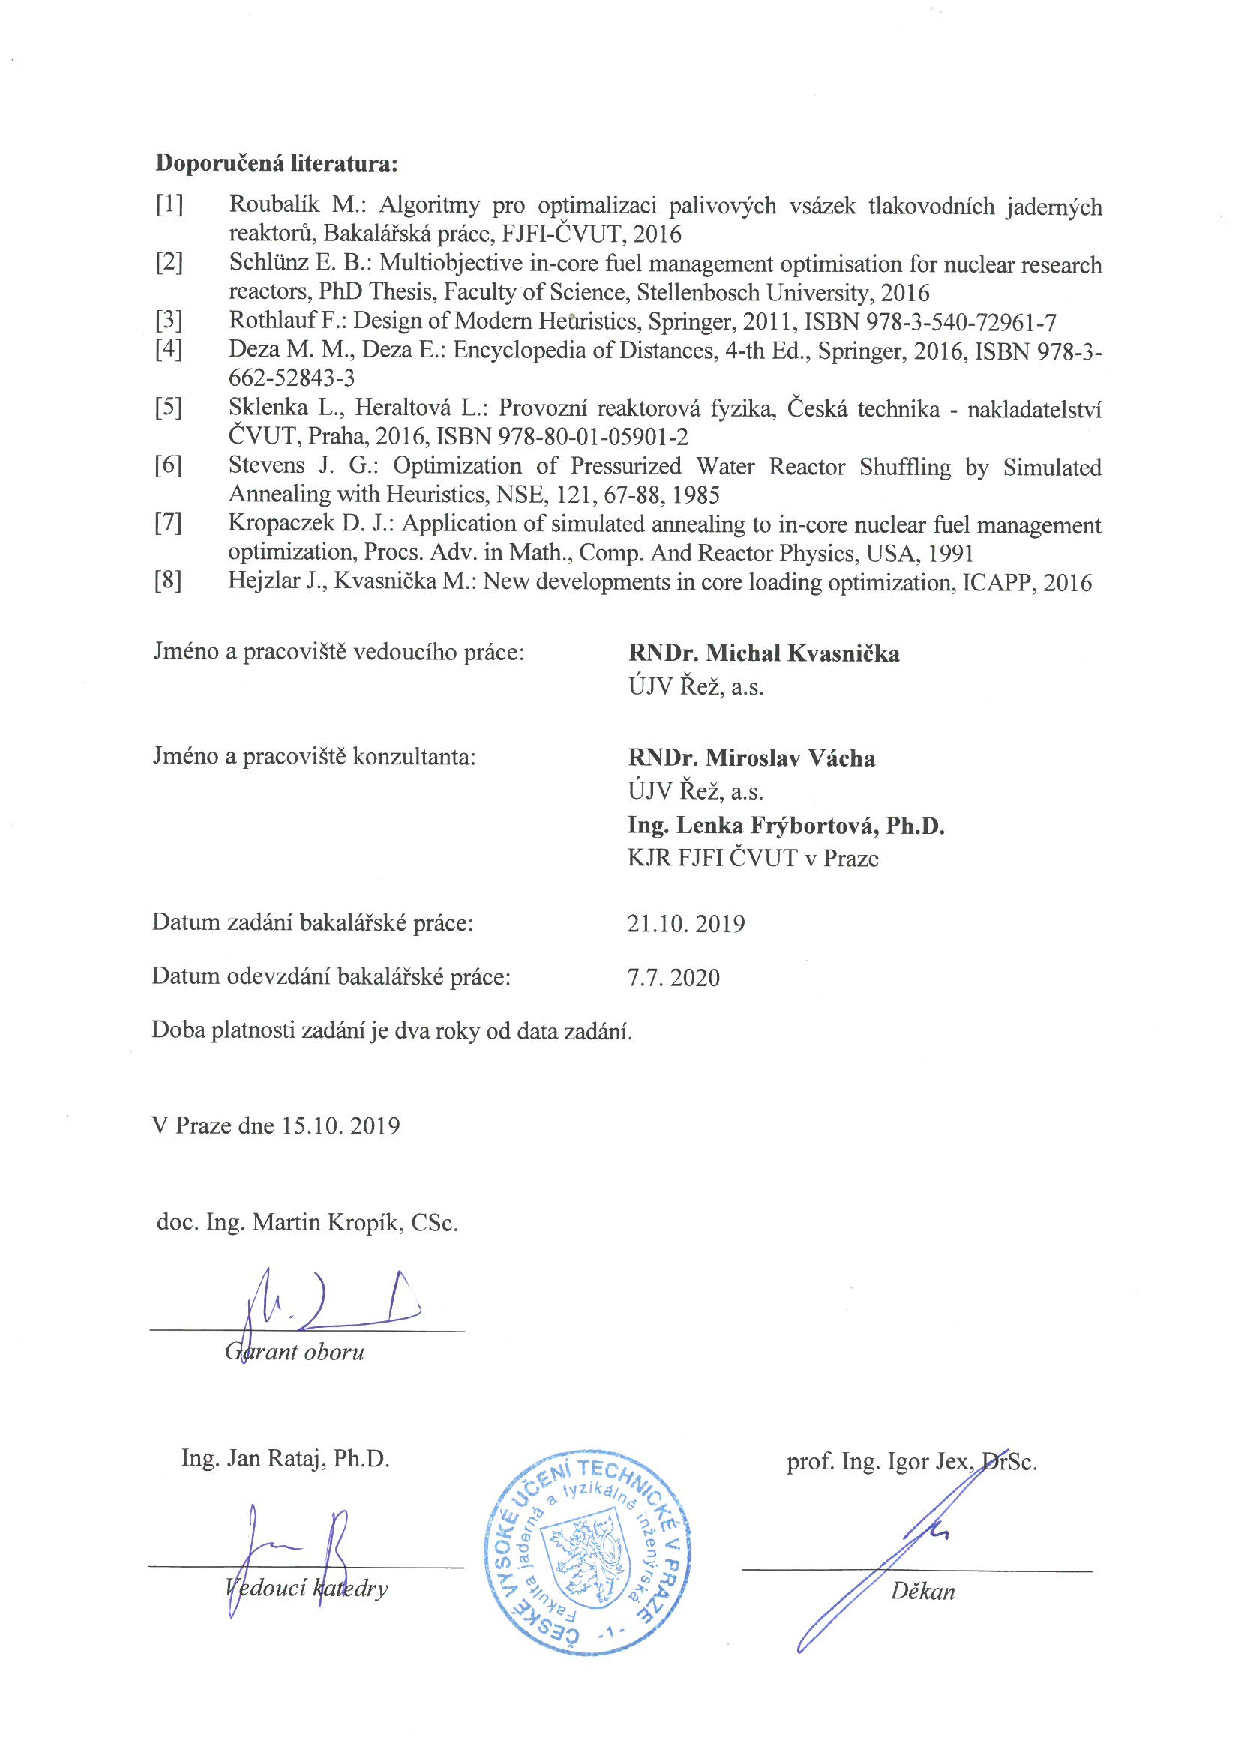
\includepdf[pages={1}]{img/bp-rzehulka-zad2.pdf}
%
%% --- varianta B: zadání naskenované jako jednotlivé stránky:
%\includepdf[pages={1}]{zadani1.pdf} % 1. strana zadání v PDF
%\includepdf[pages={1}]{zadani2.pdf} % 2. strana zadání v PDF
%
%% --- varianta C: zadání naskenované jako 2 samostatné obrázky:
%% 1. strana zadání
%\begin{center}
%     \includegraphics[width=1\textwidth]{zadani1.jpg}
%\end{center}
%% 2. strana zadání
%\newpage  % SEM NESAHEJTE!
%\thispagestyle{empty} % SEM NESAHEJTE!
%\begin{center}
%     \includegraphics[width=1\textwidth]{zadani2.jpg}
%\end{center}


%%%%%%%%%%%% Prohlášení -- SEM NESAHEJTE! Generuje se automaticky z výše nastavených maker \kde{} a \prohlaseni{}. %%%%%%%%%%%%
\newpage % SEM NESAHEJTE!
\thispagestyle{empty}  % SEM NESAHEJTE!

% SEM NESAHEJTE!
\vfill % prázdné místo. SEM NESAHEJTE!

\tb{Prohlášení} % SEM NESAHEJTE!

\vspace{1em} % vertikální mezera. SEM NESAHEJTE!
\prohlaseni

\vspace{2em}  % SEM NESAHEJTE!
\hspace{-0.5em}\begin{tabularx}{\textwidth}{X c}  % SEM NESAHEJTE!
V \kde\ dne .................... &........................................ \\	% SEM NESAHEJTE!
	& \autor
\end{tabularx}	% SEM NESAHEJTE!


%%%%%%%%%%%% Poděkování  %%%%%%%%%%%%
\newpage
\thispagestyle{empty}


\vfill % prázdné místo


% -- následující kus kódu (do "%%%%%%%%%%%% ABSTRAKT") můžete odstranit, pokud nechcete psát poděkování:
\tb{Poděkování}

\vspace{1em} % vertikální mezera
\podekovani
\begin{flushright}
\autor
\end{flushright}  % <------- tady končí stránka s poděkováním


%%%%%%%%%%%% ABSTRAKT atp. Je generován AUTOMATICKY podle maker nastavených na začátku souboru) %%%%%%%%%%%% 
\newpage   % SEM NESAHEJTE!
\thispagestyle{empty}   % SEM NESAHEJTE!

% příprava:    (na následujících 8 řádků NESAHEJTE!)
\newbox\odstavecbox
\newlength\vyskaodstavce
\newcommand\odstavec[2]{%
    \setbox\odstavecbox=\hbox{%
         \parbox[t]{#1}{#2\vrule width 0pt depth 4pt}}%
    \global\vyskaodstavce=\dp\odstavecbox
    \box\odstavecbox}
\newcommand{\delka}{120mm} % šířka textů ve 2. sloupci tabulky

% použití přípravy:    % dovnitř "tabular" vůbec NESAHEJTE!
\begin{tabular}{ll}
  {\em Název práce:} & ~ \\
  \multicolumn{2}{l}{\odstavec{\textwidth}{\bf \nazevcz}} \\[1em]
  {\em Autor:} & \autor \\[1em]
  {\em Studijní program:} & \program \\
  {\em Obor:} & \obor \\
  {\em Druh práce:} & \druh \\[1em]
  {\em Vedoucí práce:} & \odstavec{\delka}{\vedouci\\ \pracovisteVed} \\
  {\em Konzultant:} & \odstavec{\delka}{\konzultant \\ \pracovisteKonz}  % VYMAŽTE text "-- %" v případě, že jste neměli konzultanta
 \\[1em]
  & \odstavec{\delka}{\konzultantt \\ \pracovisteKonzt} \\[1em]
  \multicolumn{2}{l}{\odstavec{\textwidth}{{\em Abstrakt:} ~ \abstrCZ  }} \\[1em]
  {\em Klíčová slova:} & \odstavec{\delka}{\klicova} \\[2em]

  {\em Title:} & ~\\
  \multicolumn{2}{l}{\odstavec{\textwidth}{\bf \nazeven}}\\[1em]
  {\em Author:} & \autor \\[1em]
  \multicolumn{2}{l}{\odstavec{\textwidth}{{\em Abstract:} ~ \abstrEN  }} \\[1em]
  {\em Key words:} & \odstavec{\delka}{\keyword}
\end{tabular}



%%%%%%%%%%%% Obsah práce ... je generován AUTOMATICKY %%%%%%%%%%%%
\renewcommand\cftchapfont{\small\bfseries}
\renewcommand\cftsecfont{\footnotesize}
\renewcommand\cftsubsecfont{\footnotesize}

\renewcommand\cftchappagefont{\small\bfseries}
\renewcommand\cftsecpagefont{\footnotesize}
\renewcommand\cftsubsecpagefont{\footnotesize}

\newpage  % SEM NESAHEJTE!
\parskip=0pt
\begin{small}
\tableofcontents % SEM NESAHEJTE!
\end{small}
\parskip=7pt
\newpage % SEM NESAHEJTE!


%--------------------------------------------------------
%|         Zde začíná SAMOTNÁ PRÁCE (text)              |
%--------------------------------------------------------
%%%TODO jebni tu pod obsah seznam tabulek, seznam obrazku
% \printglossary[type=\acronymtype]

%   \printnomenclature  
%\addcontentsline{toc}{chapter}{Abbreviations}
%\printglossary[type=\acronymtype, title=Abbreviations]
\chapter*{\AcronymsWord}
\addcontentsline{toc}{chapter}{\AcronymsWord}
\markboth{\AcronymsWord}{\AcronymsWord}
\begin{acronym}[TDMA]
    \acro{ann}[ANN]{Neuronová síť (\ti{Artificial Neural Network})}
    \acro{az}[AZ]{Aktivní zóna}
\end{acronym}

\listoffigures

%%%%%%%%%%%%%%%%%%%%%%%%%%%%%%%%%%%%%%%%%%%%%%%%%%%%%%%%%%%
\mainmatter

\chapter*{Úvod} % SEM NESAHEJTE!
\addcontentsline{toc}{chapter}{Úvod} % SEM NESAHEJTE!
\markboth{Úvod}{Úvod}
\uv{Lorem ipsum} dolor sit amet, consectetur adipiscing elit. Suspendisse velit tellus, ornare at nisl vitae, mollis dignissim erat. Nulla facilisi. Nunc aliquet feugiat eros eu convallis. Donec iaculis lectus ac neque euismod ullamcorper. Cras iaculis malesuada enim ac hendrerit. Aenean porta, augue a ultricies vestibulum, tellus tellus mattis ante, sit amet efficitur tellus velit a enim. Phasellus tristique, ipsum sit amet placerat ullamcorper, turpis turpis fringilla ligula, ut mattis magna nibh id lorem. Morbi congue augue in arcu lobortis viverra. In lectus nisl, dignissim quis egestas quis, pulvinar sed odio. Mauris condimentum nisl suscipit, rutrum nibh vel, suscipit odio.

Pellentesque congue aliquet nulla quis vestibulum. Aenean vitae porttitor nunc. Praesent imperdiet erat eget justo dictum tempus. Proin pulvinar metus eget arcu elementum blandit. Duis et lacus id tellus blandit eleifend. Vestibulum eleifend molestie scelerisque. Pellentesque convallis ex sed ipsum faucibus, in fermentum nunc dignissim. Nullam eu eros non enim mattis porttitor. Nunc maximus, elit placerat elementum faucibus, eros nisi rhoncus leo, a porttitor nisl ligula ac libero. Integer fermentum eget dolor id tempus.

Something with itallic index $F_p$. And something with non-itallic $F\_p$. Sed purus enim, blandit sed interdum ut, fermentum at erat. Sed in elementum erat. In at enim nisl. Integer eu nibh sit amet quam ornare faucibus aliquam quis sem. Nunc vel nisl eu nunc congue viverra ac sagittis justo. Integer pharetra diam purus. Pellentesque dignissim est vel rutrum laoreet. Praesent id eros suscipit, porttitor nisi id, dignissim neque. Phasellus commodo volutpat nulla eget suscipit. Curabitur sit amet dapibus nisi. Donec consectetur nisl vitae neque vestibulum finibus. Duis sodales tempor ante, eu ultricies dolor bibendum ut.

Quisque id dignissim leo. Suspendisse tincidunt lacinia varius. Nunc a sem tristique, porta augue quis, tempor turpis. Pellentesque habitant morbi tristique senectus et netus et malesuada fames ac turpis egestas. Proin nulla sapien, pellentesque vitae magna sed, feugiat auctor dui. Duis nec porttitor velit. Suspendisse auctor malesuada mauris, at mattis est egestas et. Aliquam placerat molestie rutrum. Nunc tempus, est a ultricies luctus, dui leo hendrerit neque, quis dictum purus lacus et purus. Morbi aliquet elit et sodales pharetra. Morbi imperdiet viverra sagittis. Phasellus quam velit, pretium vel efficitur et, tempus ac metus. Donec non dapibus nibh. Vestibulum viverra cursus nisi. Phasellus vitae ipsum pretium, tempus mauris sagittis, tempus mi.

Maecenas dapibus erat non odio tristique porta. Suspendisse elementum nibh a nisl fermentum, eu blandit risus venenatis. Integer sed mi cursus, vestibulum dui in, gravida magna. Phasellus dictum maximus ultricies. Vivamus congue molestie ipsum, nec lobortis quam condimentum sit amet. In hac habitasse platea dictumst. Proin facilisis eleifend purus, ac egestas diam fermentum non. Aenean malesuada elit quis ligula faucibus porttitor. Etiam ornare ullamcorper orci, eget sagittis nulla fringilla ac. Ut ac metus ultricies, porttitor orci ac, accumsan erat. Nam eu elit elit. Integer vitae mi at leo elementum cursus ullamcorper eu lorem. aaaaaaaaaaaaaaa

\mdef{Parsevalova nerovnost}{parseval}{to je
Maecenas dapibus erat non odio tristique porta. Suspendisse elementum nibh a
nisl fermentum, eu blandit risus venenatis. Integer sed mi cursus, vestibulum
dui in, gravida magna. Phasellus dictum maximus ultricies. Vivamus congue
molestie ipsum, nec lobortis quam condimentum sit amet. In hac habitasse platea
dictumst. Proin facilisis eleifend purus, ac egestas diam fermentum non. Aenean
malesuada elit quis ligula faucibus porttitor. Etiam ornare ullamcorper orci,
eget sagittis nulla fringilla ac. Ut ac metus ultricies, porttitor orci ac,
accumsan erat. Nam eu elit elit. Integer vitae mi at leo elementum cursus
ullamcorper eu lorem. aaaaaaaaaaaaaaa
}

je v definici \ref{mdef:parseval}.

\mtheor{Velká Belkova}{belko}{aaaaaaaaaaaaaaaaa}

Belk citát je v~\ref{mtheor:belko}.

\mlemma{Malá Rzehulkova}{rzehulka}{PIVOOO!!!}


RRR citát je v~\ref{mlemma:rzehulka}.
\mcomm{Koment Mončin}{monca}{vám?
Quisque id dignissim leo. Suspendisse tincidunt lacinia varius. Nunc a sem tristique, porta augue quis, tempor turpis. Pellentesque habitant morbi tristique senectus et netus et malesuada fames ac turpis egestas. Proin nulla sapien, pellentesque vitae magna sed, feugiat auctor dui. Duis nec porttitor velit. Suspendisse auctor malesuada mauris, at mattis est egestas et. Aliquam placerat molestie rutrum. Nunc tempus, est a ultricies luctus, dui leo hendrerit neque, quis dictum purus lacus et purus. Morbi aliquet elit et sodales pharetra. Morbi imperdiet viverra sagittis. Phasellus quam velit, pretium vel efficitur et, tempus ac metus. Donec non dapibus nibh. Vestibulum viverra cursus nisi. Phasellus vitae ipsum pretium, tempus mauris sagittis, tempus mi.

}

Monča řekla komentář~\ref{mcomm:monca}
Quisque id dignissim leo. Suspendisse tincidunt lacinia varius. Nunc a sem tristique, porta augue quis, tempor turpis. Pellentesque habitant morbi tristique senectus et netus et malesuada fames ac turpis egestas. Proin nulla sapien, pellentesque vitae magna sed, feugiat auctor dui. Duis nec porttitor velit. Suspendisse auctor malesuada mauris, at mattis est egestas et. Aliquam placerat molestie rutrum. Nunc tempus, est a ultricies luctus, dui leo hendrerit neque, quis dictum purus lacus et purus. Morbi aliquet elit et sodales pharetra. Morbi imperdiet viverra sagittis. Phasellus quam velit, pretium vel efficitur et, tempus ac metus. Donec non dapibus nibh. Vestibulum viverra cursus nisi. Phasellus vitae ipsum pretium, tempus mauris sagittis, tempus mi.


\mex{jirka}{Jak si to máme představit?}

Jirka rekl~\ref{mex:jirka},
Quisque id dignissim leo. Suspendisse tincidunt lacinia varius. Nunc a sem tristique, porta augue quis, tempor turpis. Pellentesque habitant morbi tristique senectus et netus et malesuada fames ac turpis egestas. Proin nulla sapien, pellentesque vitae magna sed, feugiat auctor dui. Duis nec porttitor velit. Suspendisse auctor malesuada mauris, at mattis est egestas et. Aliquam placerat molestie rutrum. Nunc tempus, est a ultricies luctus, dui leo hendrerit neque, quis dictum purus lacus et purus. Morbi aliquet elit et sodales pharetra. Morbi imperdiet viverra sagittis. Phasellus quam velit, pretium vel efficitur et, tempus ac metus. Donec non dapibus nibh. Vestibulum viverra cursus nisi. Phasellus vitae ipsum pretium, tempus mauris sagittis, tempus mi.
Quisque id dignissim leo. Suspendisse tincidunt lacinia varius. Nunc a sem tristique, porta augue quis, tempor turpis. Pellentesque habitant morbi tristique senectus et netus et malesuada fames ac turpis egestas. Proin nulla sapien, pellentesque vitae magna sed, feugiat auctor dui. Duis nec porttitor velit. Suspendisse auctor malesuada mauris, at mattis est egestas et. Aliquam placerat molestie rutrum. Nunc tempus, est a ultricies luctus, dui leo hendrerit neque, quis dictum purus lacus et purus. Morbi aliquet elit et sodales pharetra. Morbi imperdiet viverra sagittis. Phasellus quam velit, pretium vel efficitur et, tempus ac metus. Donec non dapibus nibh. Vestibulum viverra cursus nisi. Phasellus vitae ipsum pretium, tempus mauris sagittis, tempus mi.
Quisque id dignissim leo. Suspendisse tincidunt lacinia varius. Nunc a sem tristique, porta augue quis, tempor turpis. Pellentesque habitant morbi tristique senectus et netus et malesuada fames ac turpis egestas. Proin nulla sapien, pellentesque vitae magna sed, feugiat auctor dui. Duis nec porttitor velit. Suspendisse auctor malesuada mauris, at mattis est egestas et. Aliquam placerat molestie rutrum. Nunc tempus, est a ultricies luctus, dui leo hendrerit neque, quis dictum purus lacus et purus. Morbi aliquet elit et sodales pharetra. Morbi imperdiet viverra sagittis. Phasellus quam velit, pretium vel efficitur et, tempus ac metus. Donec non dapibus nibh. Vestibulum viverra cursus nisi. Phasellus vitae ipsum pretium, tempus mauris sagittis, tempus mi.
Quisque id dignissim leo. Suspendisse tincidunt lacinia varius. Nunc a sem tristique, porta augue quis, tempor turpis. Pellentesque habitant morbi tristique senectus et netus et malesuada fames ac turpis egestas. Proin nulla sapien, pellentesque vitae magna sed, feugiat auctor dui. Duis nec porttitor velit. Suspendisse auctor malesuada mauris, at mattis est egestas et. Aliquam placerat molestie rutrum. Nunc tempus, est a ultricies luctus, dui leo hendrerit neque, quis dictum purus lacus et purus. Morbi aliquet elit et sodales pharetra. Morbi imperdiet viverra sagittis. Phasellus quam velit, pretium vel efficitur et, tempus ac metus. Donec non dapibus nibh. Vestibulum viverra cursus nisi. Phasellus vitae ipsum pretium, tempus mauris sagittis, tempus mi.

\chapter{Jaderný reaktor \acs{vver1000} a způsob provozu v \acs{ete}}

Za účelem lepšího popisu problematiky a vysvětlení všech souvislostí bude nejprve popsán jaderný reaktor typu \ac{vver1000} a jeho 
způsob provozování se zaměřením na bezpečnostní a ekonomické charakteristiky paliva a zóny jako celku.

\section{Popis jednotlivých částí}
%% pojmenuj to lépe

\subsection{Palivové peletky}
V současnosti je užíváno palivo TVSA-T mod. 2 ruského výrobce TVEL. Jde o peletky tvaru válce s vydutými podstavami o průměru 7,8~mm. 
% a výšce 9-12 mm. 
Palivem je \ce{^{235}U} ve formě keramického \jdt{UO_2} s průměrným obohacením do pěti procent. Ve vybraných palivových 
pletkách je přidán vyhořívající absorbátor \jdt{Gd_2O_3} s podílem 
5 \%~\cite{milisdorfer, klima}. 

\subsection{Palivový proutek}
Palivový proutek má délku 3988~mm, z níž aktivní část je 3680~mm, a průměr 9,1~mm. 
Po délce je sloupec palivových peletek, 
na koncích (posledních 150~mm aktivní délky z obou stran) tvoří blanket z peletek z přírodního \jdt{UO_2,} profilaci výkonu zajišťuje též 
umístění peletek s vyhořívajícím absorbátorem. Sloupec paliva je shora fixován pružinou (kompenzuje délkové změny během provozu, způsobené 
zejména změnami teplot). Prostor je vyplněn He o tlaku zhruba 2 MPa. Pokrytí má tloušťku 0,57~mm a 
je tvořeno slitinou E-110 (98,5~\% Zr, 1,1~\% Nb, v menší míře pak O, Fe, Hf a další~\cite{blokhin}). Zr je častým materiálem konstrukčních 
částí \ac{az} díky nízké parazitní absorpci neutronů. Jeho nevýhodou je chemické chování za vysokých teplot, kdy katalyzuje rozklad \jdt{H_2O}.
\pic{proutek.png}{Palivový proutek \acs{vver1000}.}{Popis palivového proutku pro \acs{vver1000}. Převzato z~\cite{sklenka}.}

\subsection{Palivový soubor}
Palivový soubor (\ac{ps}) je hexagonální\footnote{Typická vlastnost VVER, pocházející ze snahy o maximalizaci využití prostoru \ac{az} kvůli omezeným 
rozměrům, motivovaných transportovatelností po železnici.} a je tvořen 312 proutky, 18 vodícími trubkami a 1 centrální trubkou. Vodící i centrální trubky 
jsou z materiálu 
E-635 (96,7~\% Zr, 1,4~\% Sn, 1,1~\% Nb, dále O, Fe, Cr, Si, C a další příměsi či nečistoty v malém množství). Centrální 
trubka má význam pro nesení \ac{ps} a mohou v ní být umístěny 
samonapájecí 
detektory neutronů nebo termočlánky. Vodící trubky zajišťují (na vybraných pozicích) bezproblémový pohyb regulačních klastrů. Každý regulační klastr je 
tvořen 18 tyčemi 
s obsahem \jdt{B_4C.} Soubor je 
bezobálkový, což zlepšuje neutronovou bilanci díky menší celkové absorpci 
a termohydraulické charakteristiky (lepší promíchávání chladiva při průtoku \ac{az}). Palivové proutky jsou drženy dolním nátrubkem a 8 distančními 
mřížkami (z nichž horní a dolní jsou opatřeny směšovacími elementy k promíchávání chladiva, což zlepšuje přestup tepla, a pomáhá tak lepšímu 
rozdělení teplot po průřezu palivového souboru). Celková délka \ac{ps} je 4570~mm~\cite{ulmanova_bp, hermansky}.

\subsection{\acl{az}}
\ac{az} je tvořena 163 palivovými soubory v trojúhelníkové mříži. \ac{az} vykazuje $60\degree$ a $120\degree$ symetrii. 
Do 61 pozic se zasouvají regulační klastry. 
Klastry jsou rozdělené do 10 skupin, kde 1.~--~6. jsou bezpečnostní a během provozu jsou v horní koncové poloze, zatímco 7.~--~10. jsou pracovní. Za ustáleného 
provozu je i 7.~--~9. skupina v horní poloze a regulaci provádí 7 klastrů 10.~skupiny. Krátkodobá regulace reaktivity se tvoří pomocí klastrů a \jdt{H_3BO_3,} 
střednědobá pomocí \jdt{H_3BO_3.}

\section{Provoz VVER-1000 v ETE}
%Provoz \ac{ete} začal na v roce ..., kdy dosáhl kritičnosti ... blok. ... blok dosáhl kritičnosti .... . 

\section{Palivový cyklus}
Reaktor se provozuje kampaňovým způsobem s délkou kampaně 12~měsíců. Kampaň označuje dobu mezi dvěma odstávkami. Během odstávky se 
kontroluje (případně vyměňuje) technologie, vymění se část paliva a přeskládá aktivní zóna. Po ukončení odstávky se provádí fyzikální spouštění 
reaktoru. To zahrnuje několik testů (aktivní zóny, měřicí technologie, hermetičnosti a stavu dalších technologií) a dosahování kritičnosti. Následuje energetické 
spouštění, kdy se zvyšuje výkon až na nominální hodnotu a provádí další testování. 

Reaktor se provozuje ve čtyřletém cyklu. Cyklus označuje dobu, kterou palivo stráví v aktivní zóně. Tedy při každé odstávce se vymění zhruba 
čtvrtina paliva. 

\section{Projektování palivových vsázek}
Projektování začíná až 1,5 roku před plánovanou odstávkou. Analyzuje se palivový inventář pro danou kampaň (tj. množina palivových souborů dostupných pro 
danou kampaň, což zahrnuje čerstvé soubory ve skladu paliva, částečně použité palivo z bazénu vyhořelého paliva a použitelné palivo z aktuální 
kampaně). Následně se provádí optimalizace vsázky, tedy hledání nejlepšího přiřazení palivových souborů k pozicím v aktivní zóně, včetně rotací. 
Vhodná vsázka musí splňovat všechna bezpečnostní kritéria a zároveň maximalizovat ekonomičnost provozu. Jelikož přesné charakteristiky 
souborů z aktuální kampaně nejsou přesně známy (liší se dle konečné délky aktuální kampaně), počítá se s tzv. \ti{dlouhým} i \ti{krátkým oknem}, tj. 
dobou provozu aktuální kampaně delší i kratší než plánovaná. Pokud navrhovaná vsázka splní kritéria v obou případech, je vysoká pravděpodobnost, že 
je splní i v reálném provozu. Pokud se vhodná vsázka nenajde, je potřeba upravit palivový inventář (přidat čerstvé soubory nebo změnit obohacení). 
Na základě inventáře se pak stanoví objednávka paliva (nutno stanovit počet souborů, jejich obohacení, radiální profilování a přítomnost vyhořívajících 
absorbátorů). 

\subsection{Kritéria na vsázky}
\label{subsec:krit}
Na palivové vsázky jsou stanoveny
\cen{
\item bezpečnostní limity,
\item projekční limity,
\item provozní limity.
}

\subsubsection*{Bezpečnostní limity} stanoví výrobce paliva. Jejich hodnoty jsou stanoveny tak, aby při jejich splnění nedošlo k poškození paliva. 
Během provozu reaktoru dochází k objemovým změnám vlivem tepelné roztažnosti, od jisté teploty i k tepelnému pnutí v palivu, projevujícímu se praskáním a 
změnou tvaru (tvar \uv{bambusu}), při vyšších teplotách dochází k růstu zrn~\cite{burket_dp}. Plynová výplň zvětšuje tlak. Z paliva se mohou 
uvolňovat plyny \jdt{(H_2).} 

Interakcí pokrytí se zářením dochází k radiačnímu creepu, což vede ke zmenšení poloměru. Interakcí pokrytí s chladivem dochází k oxidaci (přičemž 
vrstva oxidu se chová jako tepelný odpor). Se vzrůstajícím vyhořením se zmenšuje mezera mezi palivem a pokrytím. Za stacionárního stavu dochází 
k určité relaxaci. Vyšší lokální výkon proutku však může vést k růstu kontaktního tlaku paliva na pokrytí, což může vést až k dehermetizaci proutku. 
Takový jev je nežádoucí a splnění bezpečnostních kritérií musí zajistit bezpečný provoz po celou dobu kampaně a udržet výše popsané jevy v přijatelných 
mezích, a garantovat tak hermetičnost paliva.

Může jít o limity na teplotu paliva, pokrytí nebo jiné veličiny týkající se mechanického či tepelného namáhání. Ty se špatně měří, proto se z bezpečnostních kritérií odvozují veličiny, které lze snadno měřit. 
Podmínky na odvozené veličiny stanovují projekční limity.
% Primární cíl optimalizace vsázek je zajištění bezpečného provozu po celou dobu kampaně. Sekundárním cílem je maximalizace ekonomičnosti provozu. 

\subsubsection*{Projekční limity} jsou stanoveny provozovatelem. Zahrnují limity odvozené z bezpečnostních limitů, limity k zajištění rezervy do krize varu, 
rovnoměrnosti výkonu (v rámci celé zóny i jednotlivých palivových souborů a proutků). Tyto limity se používají při návrhu vsázek a v následném 
bezpečnostním hodnocení. Pro \ac{ete} jsou kritéria pro návrh vsázek zahrnuta v dokumentu mini-\ac{rsac}, kritéria bezpečnostního hodnocení 
pak v \ac{rsac}. Kritéria pro vsázky zahrnují:

\tb{RCQ} limituje maximální lineární výkon axiálního úseku palivového proutku za provozu a má tvar
\eq{
	F_q  \leq F_q^{lim} K(z_i)\,,
	\label{eq:rcq_def}
}
kde 
\eq{
	F_q = 0,975 K_0 F_0^T\,.
}
$K_0$ je \ti{jaderný koeficient výkonového nevyrovnání}, který omezuje maximální relativní lineární výkon axiálního úseku 
proutku (vzhledem k jeho střednímu výkonu). 
Dosazením do definičního vztahu \eqref{eq:rcq_def} vychází
\eq{
	0,975 \operatorname*{max}\limits_{j,k,l}\(\frac{q_l^{j,k,l}}{q_l^{stř}}\)F_0^T \leq F_q^{lim} K(z_i)\,.
}
Indexy $j,k,l$ procházejí všechny palivové soubory, všechny proutky a axiální úseky, $F_0^T$ určue totální statistickou odchylku určení $K_0$, 
která zohledňuje nejistotu určení celkového výkonu a polohu proutku v rámci palivového souboru, výkon daného palivového souboru ve srovnání s celou 
zónou a počet pracujících smyček. Limitní hodnota $F_q^{lim}$ zohledňuje typ paliva a maximální povolený tepelný výkon \ac{az}. $K(z_i)$ je koeficient 
závislý na výšce daného úseku PS.

\tb{RCDH} limituje maximální relativní výkon palivového proutku 
\eq{
	F_{\Delta h} \leq F_{\Delta h}^{\mathrm{max}} = F_{\Delta H} F_r^T\,,
}
kde 
\eq{
	F_{\Delta h} = \operatorname*{max}\limits_{j,k} \frac{N_p^{j,k}}{N_p^{stř}}\,,
}
přičemž indexy $j,k$ probíhají přes všechny palivové soubory a všechny proutky. 
$F_{\Delta H}$ je maximální hodnota relativního výkonu palivového proutku a $F_r^T$ 
je součinitel zohledňující nejistoty měření a výrobní tolerance.

\tb{RCHA} limituje maximální relativní výkon palivového souboru $K_q$
\eq{
	K_q = \operatorname*{max}\limits_{j} \frac{N_{PS}^{j}}{N_{PS}^{stř}} \leq K_q^{lim}\,,
}
kde $j$ probíhá přes všechny palivové soubory v \ac{az}.


\tb{\ac{rc1}} je maximální lineární výkon axiálního úseku palivového proutku $q_l^{ax}$ v závislosti na středním 
vyhoření palivového proutku, ve kterém se daný úsek nachází. 
Za provozu musí být splněno kritérium
\eq{
	q_l^{ax}\cdot \(F_0^{inž}(\bar{r})F^I \) \leq q_l^{ax\_lim}\,,
}
kde $F_0^{inž}(\bar{r})F^I$ je inženýrský faktor, resp. faktor neurčitosti; jejich součin určuje celkovou nejistotu~\cite{ulmanova_bp}. Limitní hodnoty $q_l^{ax\_lim}$ jsou
%% TODO
závislé na přítomnosti vyhořívajících absorbátorů a hodnoty pro \ac{ete} jsou uvedeny v tabulce~\ref{tab:rc1_lims}~\cite{ulmanova_ing}. 
\begin{table}[H]
\centering
\caption{Limity pro $q_l^{ax\_lim}$ [\jdt{W\cdot cm^{-1}}] při použití paliva tvel (bez Gd), resp. tveg (s Gd) v ETE. Převzato z~\cite{ulmanova_ing}.}
\label{tab:rc1_lims}
\begin{tabular}{|c|c|c|c|}
\hline
\multicolumn{2}{|c|}{Proutky bez \jdt{Gd_2O_3}} & \multicolumn{2}{c|}{Proutky s \jdt{Gd_2O_3}} \\ \hline
\acs{bu} $\left[\frac{\jde{MWd}}{\jde{kgU}}\right]$ & $q_l^{ax\_lim} \left[\frac{\jde{W}}{\jde{cm}}\right]$ & \acs{bu} $\left[\frac{\jde{MWd}}{\jde{kgU}}\right]$ & $q_l^{ax\_lim} \left[\frac{\jde{W}}{\jde{cm}}\right]$ \\ \hline
0 & 448 & 0 & 360 \\ \hline
20 & 362 & 15 & 360 \\ \hline
40 & 312 & 35 & 310 \\ \hline
75 & 252 & 70 & 255 \\ \hline
\end{tabular}
\end{table}

Parametr \ac{rc1} je v procesu optimalizace maximalizován (za splnění restrikčních podmínek). 

\tb{RC3} omezuje skok lokální hustoty výkonu proutku na začátku cyklu v závislosti na jeho lokálním vyhoření. 

%\tb{RC4}

\tb{\ac{mtc}} ($a_T^M$) je definovaný jako
\begin{scriptsize}
\eq{
	a_T^M = \frac{\partial \rho}{\partial T_M} = \frac{1}{k_{eff}^2}\left[\underbrace{\varepsilon\eta p f \pder{P_{NL}}{T_M}}_\text{1} + \underbrace{P_{NL} \eta p f \pder{\varepsilon}{T_M}}_\text{2} + \underbrace{P_{NL}\varepsilon p f \pder{\eta}{T_M}}_\text{3} + \underbrace{P_{NL}\varepsilon\eta f \pder{p}{T_M}}_\text{4} + \underbrace{P_{NL}\varepsilon\eta p \pder{f}{T_M}}_\text{5} \right]\,.
	\label{eq:mtc_def}
}
\end{scriptsize}
Vliv jednotlivých členů je rozebrán níže.
\cen{
\item Ze vztahu pro $P_{NL}$ 
	\eq{
		P_{NL} = \frac{1}{(1+B^2 L_T^2)(1+B^2 \tau_T)}
	}
	plyne, že první člen v součtu \eqref{eq:mtc_def} je záporný, protože $L_T^2$ i $\tau_T$ rostou s teplotou. To plyne 
	z jejich definice. Difuzní plocha $L_T^2$, definovaná jako
	\eq{
		L_T^2 = \frac{\bar{D}}{\bar{\Sigma}_a}\,,
	}
	s teplotou roste, protože rostoucí závislost
	\eq{
		\bar{D}(T) = \Gamma (m+2) D(E_0) \( \frac{T}{T_0}\)^m\,,
	}
	kde $m$ je konstanta daná typem moderátoru (pro \jdt{H_2 O} $m = 0,470$), je dominantní oproti závislosti $\Sigma_a (T)$~\cite{zaf2Kinetika}. 
	Stáří neutronů (dle~\cite{enf}) 
	\eq{
		\tau_T = \frac{\bar{r^2}(E_0,E)}{6}
	}
	s teplotou roste v důsledku zhoršených moderačních schopností (způsobených poklesem hustoty \jdt{H_2 O}). Zvýšení energie, na kterou jsou 
	neutrony zpomalovány, má zanedbatelný záporný vliv na $\tau_T$~\cite{zaf2Kinetika}. 

\item Závislost koeficientu násobení rychlými neutrony $\varepsilon(T_M)$ je malá~\cite{zaf2Kinetika}.
%% TODO Tím si nejsem jist!!!

\item Regenerační faktor $\eta$ charakterizuje palivo, proto je na teplotě moderátoru nezávislý~\cite{zaf1Stepeni}.

\item Závislost pravděpodobnosti úniku rezonančnímu záchytu $p(T_M)$ má záporný efekt, což je důsledkem zhoršených moderačních schopností \jdt{H_2 O} 
	(v důsledku poklesu hustoty)~\cite{sklenka}. 
\item S rostoucí teplotou (a tedy i objemem) \jdt{H_2 O} klesá koncentrace \jdt{H_3 BO_3,} dochází tak ke snížení absorpce a efekt je kladný~\cite{sklenka}.
}

\ac{mtc} představuje nejvýznamnější příspěvek k záporné teplotní vazbě reaktoru (což je základní předpoklad bezpečného 
provozu reaktoru a nutná podmínka k udělení licence k provozu dle \ac{sujb}). Dle legislativy 
musí být $\ac{mtc}<0$ za všech provozních stavů. \ac{mtc} je nejvyšší během spouštění, a to z důvodu vysoké koncentrace \jdt{H_3BO_3.} 
K zajištění záporných hodnot se zavádí dolní mez teploty \ac{az}. Spouštění je možné provést jen tehdy, je-li teplota \ac{az} větší než stanovené 
minimum~\cite{sklenka, hezoucky}. 

Záporné zpětné vazby jsou žádoucí i pro ekonomičnost provozu. Provoz začíná při určité výšce pracovní skupiny regulačních klastrů (různé od horní 
koncové polohy) a s určitou koncentrací \jdt{H_3BO_3.} V průběhu kampaně vyhořívá palivo, tj. ubývá štěpných izotopů a klesá reaktivita 
paliva. To se kompenzuje
\cit{
\item vyhořívajícími absorbátory (Gd vnáší zápornou reaktivitu, jejíž množství vlivem rozpadu klesá -- průběh $\rho(t)$ se od zóny bez 
	vyhořívajících absorbátorů liší \textasciitilde 150 dní, poté se průběh téměř neliší od lineárního poklesu),
\item poklesem koncentrace \jdt{H_3BO_3} (např.: 13. kampaň 1. bloku \ac{ete} začala na koncentraci $9,2~\jde{g/kg}$ s rychlým 
	poklesem na $6,7~\jde{g/kg}$ při vyhoření $\approx~5$ \ac{efpd} a s následným lineární poklesem na $0~\jde{g/kg}$ při vyhoření 285 \ac{efpd}), 
\item vytahováním pracovní skupiny regulačních klastrů do horní koncové polohy (řádově jednotky cm za den).
}

Po dosažení nulové koncentrace \jdt{H_3BO_3} a horní koncové polohy regulačních klastrů pokračuje provoz na \ti{teplotním} a \ti{výkonovém efektu}. 
Při provozu na teplotním a výkonovém efektu dochází k poklesu tlaku v hlavním parním kolektoru. To zlepšuje odvod tepla z primárního okruhu, a tedy 
dochází ke snížení teploty na vstupu do reaktoru. Vlivem záporného koeficientu reaktivity na teplotu moderátoru dochází k zvýšení reaktivity a 
reaktor se udržuje na nominálním výkonu. Tomu se říká teplotní efekt a prodlužuje nominální provoz až o pět dní. Poté dochází k poklesu výkonu 
rychlostí cca 1 \% za den. Tím se snižuje stacionární xenonová otrava, a tedy klesá zásoba záporné reaktivity a provoz se prodlužuje, 
a to o 15 až 20 dní. 
Provoz na efektech celkově prodlužuje kampaň o 20 až 25 dní~\cite{sklenka}.

V praxi se \ac{mtc} počítá neutronickým kódem, protože jej nelze 
měřit -- teplota paliva a moderátoru se mění současně. 
K měření se zavádí izotermický teplotní koeficient 
(\ac{itc}) vztahem \ac{itc} = \ac{mtc} + \ac{dtc}. Měření \ac{itc} vyžaduje provádění rovnoměrných změn teploty. To je možné provádět v průběhu fyzikálního 
spouštění, 
% \footnotei{,}{Rozlišuje se \ti{fyzikální} a \ti{energetické} spouštění. Před spouštěním se provádí kontrola těsnosti a provozních celků 
% primárního i sekundárního okruhu. Fyzikální spouštění zahrnuje dosažení kritického stavu na úrovni $10^{-6}\%$ nominálníh výkonu (tzv. minimálního 
% kontrolovatelného výkonu -- \ti{MKV}). Poté dojde k ohřátí chladiva na provozní teplotu a minimalizuje se odvod tepla z primárního okruhu. Tím se dosáhne 
% tepelné rovnováhy mezi palivem a chladivem, kdy se měří ITC. Následují testy dalších komponent priárního okruhu a jsou-li úspěšné, začne se zvyšovat 
% výkon na nominální hodnotu. Následují testy energetického spouštění \cite{sklenka}.}
kdy je reaktor v horkém stavu při nulovém výkonu (stav reaktoru při \ac{mkv}, kdy nepůsobí teplotní zpětné vazby)~\cite{sklenka}. 

Při běhu programu LPopt tvoří \ac{mtc} restrikční podmínku kladenou na optimální řešení $\ac{mtc}<0$.


\subsubsection*{Provozní limity} jsou stanoveny provozovatelem a jejich splnění se kontroluje za provozu. Jejich definice zahrnuje výrobní tolerance 
a nejistoty měřícího systému. 

\subsection{Optimalizační program LPopt}
V procesu optimalizace vsázek je na \ac{ete} v současnosti používán program LPopt, vyvinutý v \ac{ujv} Řež, a.~s. Základem je generování 
vsázek na základě algoritmu třídy \ac{eda} \cite{roubalik} ve spojení s programem Andrea 2D, který vyhodnocuje odezvy \ac{bc} \ac{eoc}, \ac{fdh}, \ac{fha}, 
\ac{rc1}, \ac{pbu}, \ac{mtc}. Proces je vedený k minimalizaci \ac{fdh} za současné maximalizace \ac{rc1}. Vhodné vsázky musí zároveň splňovat 
kritéria na \ac{bc} \ac{eoc}, \ac{fha}, \ac{pbu} a \ac{mtc}. 

\ac{bc} \ac{eoc} má význam pro délku cyklu a je snaha ji maximalizovat. Udává se v jednotkách \jdt{g\cdot kg^{-1}} a má záporné hodnoty, což souvisí 
s poklesem koncentrace na nulovou během kampaně a následným provozem na teplotním a výkonovém efektu, popsaném v části~\ref{subsec:krit}, odstavec 
\ac{mtc}. Záporná koncentrace nemá fyzikální smysl, jde o extrapolaci lineárního poklesu během kampaně (graf koncentrace \ac{bc} v závislosti na vyhoření 
je na obr.~\ref{bc_ete.png}). Optimalizace \ac{bc} \ac{eoc} je výhodnější než přímá optimalizace efektivní délky 
cyklu\footnotei{.}{Zdůvodnění tohoto jevu je však nad rámec této práce.}

\ac{pbu} je vyhodnocováno z důvodu vícecyklové optimalizace -- je žádoucí v rámci palivového cyklu maximalizovat vyhoření, ale je nutno brát 
v úvahu zajištění dostatku \ac{ps} pro následující kampaň. Hodnota \ac{pbu} slouží jako restrikční podmínka. 

Potřeba hodnocení ostatních čtyř parametrů (\ac{fdh}, \ac{fha}, \ac{rc1}, \ac{mtc}) je dána projekčními kritérii zmíněnými výše.

\pic{bc_ete.png}{Průběh \ac{bc} během kampaně \ac{ete}.}{Vypočtená závislost kritické \ac{bc} na \ac{bu} pro 13. kampaň 1. bloku \ac{ete}. Rychlý pokles v prvních dnech kampaně souvisí s energetickým spouštěním. Následný lineární pokles je daný postupným vyhoříváním a tedy menším přebytkem reaktivity nutným kompenzovat. Převzato z~\cite{sklenka}.}

% \section{Testovací data}
% V numerických pokusech byla použita data z běhu optimalizačního programu LPopt pro 15. cyklus 1. bloku jaderné elektrárny Temelín (\verb|u1c15|). 
% Vsázky byly generované programem LPopt, je zachycen celý optimalizační proces. Data tedy nejsou náhodně vzorkovaná, hodnoty jsou vychýlené 
% (důsledek cíle LPopt -- minimalizace \ac{fdh} při současné maximalizaci \ac{rc1}. Soubor obsahoval 
% $10^6$ vsázek (přiřazení palivového souboru a jeho rotace ke každé pozici v AZ), vybrané odezvy 
% (veličiny \ac{bc}, \ac{fdh}, \ac{fha}, \ac{rc1},\ac{pbu}, \ac{mtc}) 
% vypočtené neutronickým kódem Andrea 2D (méně přesný, ale pro účely optimalizace postačující --  používá se kvůli zrychlení výpočtu -- $\approx 0,3$ s na 
% vsázku při jednom CPU jádře oproti 30--60 s v 3D režimu) a fyzikální parametry všech uvažovaných palivových souborů -- 121 veličin 
% pro každý -- zahrnující informace 
% o složení (množství důležitých izotopů), použití (vyhoření, výkon) a vypočtené účinné průřezy (pro jednu a dvě grupy) -- bližší popis je 
% v příloze~\ref{app:params}.
% 
% Dataset tvořila matice $\mathcal{C}$ rozměru $(10^6, 56)$, jejíž řádky obsahovaly vektory $\bv{c}$ (definovány dle \ref{ch:repr}) jednotlivých 
% vsázek. Odezvy byly v matici $\mathcal{R}$ rozměru $(10^6, 6)$, jejíž řádky odpovídaly odezvám \ac{az} s konfigurací popsanou příslušným 
% řádkem v $\mathcal{C}$. 
% Dále byla přiložena tabulka \ac{fap} rozměru (150, 121), jejíž řádky obsahovaly fyzikální parametry palivových souborů v jednotlivých rotacích. 
% Matice $\bv{P}$ se vytvořila přiřazením řádků tabulky s palivem ke složkám $\bv{c}$.
% 
% K dispozici bylo 25 palivových souborů s parametry vypočtenými pro všechny rotace (tj. celkem $150 = 25\cdot6$ různých \ac{ps}). Seznam 
% fyzikálních parametrů, popisujících palivové soubory, 
% je v příloze \ref{app:params}. 
% %Veličiny tvořící výstup z neutronického kódu jsou popsány níže. 
% Odezvy jsou veličiny vyhodnocované 
% v průběhu optimalizačního programu LPopt -- koncentraci \jdt{H_3BO_3} EOC, koeficient poproutkového nevyrovnání \ac{fdh}, 
% koeficient pokazetového nevyrovnání \ac{fha} ($=K_q$), parametr \ac{rc1}, maximální poproutkové vyhoření (\ac{pbu}) a hodnotu \ac{mtc}.







% \subsubsection*{Koncentrace \jdt{H_3BO_3} na konci cyklu}
% Koncentrace \jdt{H_3BO_3} na konci cyklu (\verb|bc|, \ti{BorinAcid EOC}) je 
% 
% \subsubsection*{Koeficient nevyrovnanosti výkonu proutku}
% Během procesu optimalizace se tento koeficient minimalizuje. 
% \subsubsection*{Koeficient nevyrovnanosti výkonu souboru}

% \subsubsection*{Bezpečnostní parametr \ac{rc1}}
% \ac{rc1} je maximální lineární výkon axiálního úseku palivového proutku $q_l^{ax}$ v závislosti na středním 
% vyhoření palivového proutku, ve kterém se daný úsek nachází. 
% Za provozu musí být splněno kritérium
% \eq{
% 	q_l^{ax}\cdot \(F_0^{inž}(\bar{r})F^I \) \leq q_l^{ax\_lim}\,,
% }
% kde $F_0^{inž}(\bar{r})F^I$ je inženýrský faktor, resp. faktor neurčitosti; jejich součin určuje celkovou nejistotu \cite{ulmanova_bp}. Limitní hodnoty $q_l^{ax\_lim}$ jsou
% %% TODO
% závislé na přítomnosti vyhořívajících absorbátorů a hodnoty pro \ac{ete} jsou uvedeny v tabulce~\ref{tab:rc1_lims}. 
% \begin{table}[H]
% \centering
% \caption{Limity pro $q_l^{ax\_lim}$ [\jdt{W\cdot cm^{-1}}] při použití paliva tvel (bez Gd), resp. tveg (s Gd) v ETE. Převzato z \cite{ulmanova_ing}.}
% \label{tab:rc1_lims}
% \begin{tabular}{|c|c|c|c|}
% \hline
% \multicolumn{2}{|c|}{Proutky bez \jdt{Gd_2O_3}} & \multicolumn{2}{c|}{Proutky s \jdt{Gd_2O_3}} \\ \hline
% \ac{bu} $\left[\frac{\jde{MWd}}{\jde{kgU}}\right]$ & $q_l^{ax\_lim} \left[\frac{\jde{W}}{\jde{cm}}\right]$ & \ac{bu} $\left[\frac{\jde{MWd}}{\jde{kgU}}\right]$ & $q_l^{ax\_lim} \left[\frac{\jde{W}}{\jde{cm}}\right]$ \\ \hline
% 0 & 448 & 0 & 360 \\ \hline
% 20 & 362 & 15 & 360 \\ \hline
% 40 & 312 & 35 & 310 \\ \hline
% 75 & 252 & 70 & 255 \\ \hline
% \end{tabular}
% \end{table}
% 
% Parametr \ac{rc1} je v procesu optimalizace maximalizován (za splnění restrikčních podmínek). 

% \subsubsection*{Maximální poproutkové vyhoření}

% \subsubsection*{Moderátorový teplotní koeficient reaktivity}
% Moderátorový teplotní koeficient reaktivity (\verb|mtc|, $a_T^M$) je definovaný jako
% \begin{scriptsize}
% \eq{
% 	a_T^M = \frac{\partial \rho}{\partial T_M} = \frac{1}{k_{eff}^2}\left[\epsilon\eta p f \pder{P_{NL}}{T_M} + P_{NL} \eta p f \pder{\epsilon}{T_M} + P_{NL}\epsilon p f \pder{\eta}{T_M} + P_{NL}\epsilon\eta f \pder{p}{T_M} + P_{NL}\epsilon\eta p \pder{f}{T_M} \right]
% 	\label{eq:mtc_def}
% }
% \end{scriptsize}
% % Při změně teploty moderátoru dochází 
% 
% \cen{
% \item Ze vztahu pro $P_{NL}$ 
% 	\eq{
% 		P_{NL} = \frac{1}{(1+B^2 L_T^2)(1+B^2 \tau_T)}
% 	}
% 	plyne, že první člen v součtu \eqref{eq:mtc_def} je záporný, protože $L_T^2$ i $\tau_T$ rostou s teplotou. To plyne 
% 	z jejich definice. Difuzní plocha $L_T^2$, definovaná jako
% 	\eq{
% 		L_T^2 = \frac{\bar{D}}{\bar{\Sigma}_a}\,,
% 	}
% 	s teplotou roste, protože rostoucí závislost
% 	\eq{
% 		\bar{D}(T) = \Gamma (m+2) D(E_0) \( \frac{T}{T_0}\)^m\,,
% 	}
% 	kde $m$ je konstanta daná typem moderátoru (pro \jdt{H_2 O} $m = 0,470$), je dominantní oproti závislosti $\Sigma_a (T)$ \cite{zaf2Kinetika}. 
% 	Stáří neutronů \cite{enf} 
% 	\eq{
% 		\tau_T = \frac{\bar{r^2}(E_0,E)}{6}
% 	}
% 	s teplotou roste v důsledku zhoršených moderačních schopností (způsobenými poklesem hustoty \jdt{H_2 O}). Zvýšení energie, na kterou jsou 
% 	neutrony zpomalovány, má zanedbatelný záporný vliv na $\tau_T$ \cite{zaf2Kinetika}. 
% 
% \item Závislost koeficientu násobení rychlými neutrony $\epsilon(T_M)$ je malá \cite{zaf2Kinetika}.
% %% TODO Tím si nejsem jist!!!
% 
% \item Regenerační faktor $\eta$ charakterizuje palivo, proto je na teplotě moderátoru nezávislý \cite{zaf1Stepeni}.
% 
% \item Závislost pravděpodobnosti úniku rezonančnímu záchytu $p(T_M)$ má záporný efekt, což je důsledkem zhoršených moderačních schopností \jdt{H_2 O} 
% 	(v důsledku poklesu hustoty) \cite{sklenka}. 
% \item S rostoucí teplotou (a tedy i objemem) \jdt{H_2 O} klesá koncentrace \jdt{H_3 BO_3}, dochází tak ke snížení absorpce a efekt je kladný \cite{sklenka}.
% }
% 
% MTC představuje nejvýznamnější příspěvek k záporné teplotní vazbě reaktoru (což je základní předpoklad bezpečného 
% provozu reaktoru a nutná podmínka k udělení licence k provozu dle SÚJB). Dle legislativy 
% musí být $\jde{MTC}<0$ za všech provozních stavů. MTC je nejvyšší během spouštění a to z důvodu vysoké koncentrace \jdt{H_3BO_3}. 
% K zajištění záporných hodnot se zavádí dolní mez teploty AZ. Spouštění je možné provést jen tehdy, je-li teplota AZ větší, než stanovené 
% minimum \cite{sklenka}, \cite{hezoucky}. 
% 
% Záporné zpětné vazby jsou žádoucí i pro ekonomičnost provozu. Provoz začíná při určité výšce pracovní (různé od horní koncové polohy) skupiny 
% regulačních klastrů a s určitou koncentrací \jdt{H_3BO_3}. V průběhu kampaně vyhořívá palivo, tj. ubývá štěpných izotopů a klesá reaktivita od 
% paliva. To se kompenzuje
% \cit{
% \item vyhořívajícími absorbátory (Gd vnáší zápornou reaktivitu, jejíž množství vlivem rozpadu klesá -- průběh $\rho(t)$ se od zóny bez 
% 
% 	vyhoř. abs. liší \~150 dní, poté se průběh téměř neliší od lineárního poklesu),
% \item poklesem koncentrace \jdt{H_3BO_3} (např.: 26. kampaň EDU začala na konc. $> 9 \jde{g/kg}$, následoval rychlý pokles na $\approx 5,7 \jde{g/kg}$, 
% 	následován pomalým lineárním poklesem do 0 v čase \~340 dní),
% \item vytahováním pracovní skupiny regulačních klastrů do horní koncové polohy (řádově jednotky cm za den).
% }
% 
% Po dosažení nulové koncentrace \jdt{H_3BO_3} a horní koncové polohy regulačních klastrů pokračuje provoz na \ti{teplotním} a \ti{výkonovém efektu}. 
% Při provozu na teplotním a výkonovém efektu dochází k poklesu tlaku v hlavním parním kolektoru. To zlepšuje odvod tepla z primárního okruhu a tedy 
% dochází ke snížení teploty na vstupu do reaktoru. Vlivem záporného koeficientu reaktivity na teplotu moderátoru dochází k zvýšení reaktivity a 
% reaktor se udržuje na nominálním výkonu. Tomu se říká teplotní efekt a prodlužuje nominální provoz až o pět dní. Poté dochází k poklesu výkonu 
% rychlostí \~1\% za den. Tím se snižuje stacionární xenonová otrava a tedy klesá zásoba záporné reaktivity a provoz se prodlužuje, a to o 15 až 20 dní. 
% Provoz na efektech celkově prodlužuje kampaň o 20 až 25 dní \cite{sklenka}.
% 
% MTC nelze za provezu měřit, protože teplota paliva a moderátoru se mění současně. Proto se zavádí měřitelný izotermický teplotní koeficient 
% (ITC, \ti{isotermic temperature coefficient}) vztahem ITC = MTC + DTC, kde DTC je teplotní koeficient reaktivity od paliva (\ti{Doppler 
% temperature coefficient}). Měření ITC vyžaduje provádění rovnoměrných změn teploty. To je možné provádět v průběhu fyzikálního 
% spouštění\footnotei{,}{Rozlišuje se \ti{fyzikální} a \ti{energetické} spouštění. Před spouštěním se provádí kontrola těsnosti a provozních celků 
% primárního i sekundárního okruhu. Fyzikální spouštění zahrnuje dosažení kritického stavu na úrovni $10^{-6}\%$ nominálníh výkonu (tzv. minimálního 
% kontrolovatelného výkonu -- \ti{MKV}). Poté dojde k ohřátí chladiva na provozní teplotu a minimalizuje se odvod tepla z primárního okruhu. Tím se dosáhne 
% tepelné rovnováhy mezi palivem a chladivem, kdy se měří ITC. Následují testy dalších komponent priárního okruhu a jsou-li úspěšné, začne se zvyšovat 
% výkon na nominální hodnotu. Následují testy energetického spouštění \cite{sklenka}.} 
% kdy je reaktor v horkém stavu při nulovém výkonu (stav reaktoru při MKV, kdy nepůsobí teplotní zpětné vazby) \cite{sklenka}. 
% %Hodnoty \ac{mtc} a DTC se musí získávat pomocí \ti{online výpočtů}.
% 
% Při běhu programu LPopt tvoří \ac{mtc} restrikční podmínku kladenou na optimální řešení $\jde{MTC}<0$.

%-- konkrétně veličiny bc, fdh, fha, rc1, pbu, mtc. 

% Palivový inventář obsahoval 25 palivových souborů. 
% Každý soubor byl (pro každou rotaci) popsán vektorem 121 fyzikálních parametrů (uvedeny v příloze \ref{app:params}). Každá vsázka 
% byla popsána vektorem $\bv{c}$. 

\chapter{Obecná formulace optimalizace vsázek}

\section{Definice, přístupy}
Optimalizací palivových vsázek (\ac{lpo}, též \ac{micfmo})
se rozumí hledání nejlepší konfigurace paliva, regulačních orgánů 
a vyhořívajících absorbátorů v aktivní zóně. Optimalizace zahrnuje výběr palivových souborů, 
jejich umístění a rotaci a výběr množství a umístění 
vyhořívajících absorbátorů. Úloha je omezena dostupným palivem 
(zahrnujícím čerstvé a částečně vyhořelé soubory)
a bezpečnostními kritérii. Bezpečnostní kritéria a proces hodnocení jsou stanoveny v interních dokumentech 
provozovatele.

Podle palivového inventáře rozlišujeme \ti{incore} a \ti{excore} optimalizaci~\cite{roubalik}.
\cen{
	\item \textit{Incore} optimalizace je úloha přiřazení $m = n$ palivových elementů k $n$ pozicím v symetrické části \ac{az} (pro zjednodušení výpočtu se \ac{az} rozdělí na několik symetrických částí (v případě \ac{vver} na 6).
	\item \textit{Excore} optimalizace více odpovídá reálnému provozu -- $m > n$, tedy nejde pouze o umístění palivových souborů, ale i o vhodný výběr souborů z inventáře, který je obecně větší než počet pozic v \ac{az}. Dále se optimalizují délky cyklů.%TODO roubalik
}
Z hlediska počtu cyklů se rozlišuje jednocyklová a vícecyklová optimalizace. 
\cen{
		\item Jednocyklová optimalizace (\ac{icfmo}) zahrnuje návrh pouze jednoho cyklu. To může vést k nevýhodnému palivovému inventáři pro 
			následující cykly. 
		\item Vícecyklová optimalizaci (\ac{ocfmo}) optimalizuje více cyklů dopředu, tj. bere v úvahu, že výstup jednoho cyklu 
			ovlivňuje vstup následujícího. Úloha je výrazně náročnější (např. je potřeba modelovat izotopické složení palivových souborů 
			na konci cyklu). Nejistota výpočtů roste s množstvím dopředu plánovaných cyklů, navíc může docházet 
			k neplánovaným změnám (objevení netěsnosti či jiného poškození palivového souboru, neplánovaná odstávka). To 
			způsobuje, že optimalizace na mnoho cyklů dopředu může být nepraktická. Je možné použít předpoklad, že 
			\ac{icfmo} ovlivní \ac{ocfmo} jen omezeně. \ac{ocfmo} pak stanoví požadavky na \ac{icfmo}~\cite{schlunz}. 
			%To je potřeba brát v úvahu a optimalizovat více cyklů dopředu, což úlohu komplikuje -- je potřeba 
			%modelovat izotopické složení palivových souborů, 
}

%% ISSUES
%% ===============================================
%% palivová vsázka, překládkové schéma,... -- co je co?
%% co všechno optimalizujeme
%% rozdíl mezi kampaní a cyklem, jak je dlouhé u jednotlivých reaktorů, upřesnit!!!
%% které veličiny maximalizujeme, kde je to psané, metodika hodnocení
%% jaká jsou bezpečnostní omezení a kde jsou specifikována
%% rozdil -- metody incore a outcore
%% rozdil -- 1 cyklova a vicecyklova -- jak je v praxi

%% Solved
%% ============
%% palivový soubor = ETE, 163 v zone, 6-úh, bezobálkový, tvořený 312 paliv. proutky, 18 vodícími trubkami a centrální trubkou
%% palivová kazeta = EDU, 349 v zone, 6-uh, obálkové,126 tyčí,  -- cite sklenka, hermansky


\section{Vlastnosti problému optimalizace vsázek}
\label{ch:vlastnosti}
% \ti{LPO} se označuje také jako \ti{MICFMO} (\ti{Multi-objective In-Core Fuel Management Optimization}). 
Matematicky je \ac{micfmo} úloha vícekriteriálního optimálního 
nelineárního přiřazení s omezujícími podmínkami (\ti{constrained})~\cite{roubalik}. Specifické vlastnosti užitkové funkce a prostorů, 
na kterých operuje, budou rozebrány podrobněji 
v kapitole \ref{ch:new}. Vlastnosti problému jako celku budou rozebrány níže. Bližší popis některých vlastností uvádí článek~\cite{stevens}.

% %% nadefinovat MICFMO, omezující podmínky, kombinatorické kecy, omezující podmínky, pareto frontu, suboptimální vsázku, penalizace, Stevensovy vl.,
% %% objective fx

% zdůraznit rozdíl mezi diskrétní a spojitou optimalizací


\subsection{Diskrétnost}
\label{sec:diskretnost}
Záměna palivových souborů se děje vždy diskrétně. To omezuje přístup k řešení problému -- mnoho analytických metod 
nelze použít, protože jsou založeny na spojitých změnách. Proto je nutné použít metody k diskrétním problémům -- podobně 
jako u \ti{problému obchodního cestujícího}-je možno prohledat část prostoru vsázek pomocí diskrétních kroků. 
Prostor z principu nelze prohledat celý. 

\ac{az} typu \ac{vver1000} o 163 palivových pozicích s uvážením rotací má 
\eq{
	6^{163}\cdot 163!
}
teoretických 
	vsázek, navíc v palivovém inventáři elektrárny (sklad čerstvého paliva, bazén použitého paliva a aktuální obsah aktivní zóny) 
	může být víc palivových souborů než pozic v \ac{az}. Je-li $m$ počet souborů v inventáři, bude maximální počet vsázek 
	shora omezen $\binom{m}{163} 163! 6^{163}$. 
	Reálný počet je však menší -- soubory se opakují, \ac{az} je symetrická (u \ac{vver1000} jde o šestinovou symetrii). S využitím symetrie se optimalizuje pouze $28$ pozic -- tomu odpovídá 
	\eq{
		\binom{m}{28} 28! 6^{28} > 10^{52}\,.
	}
	Restriktivní podmínky spoustu vsázek zamítnou -- např. z požadavku na nízkoúnikové vsázky 
	se čerstvé kazety neumisťují na okraj zóny. Některé rotace konkrétního souboru v určité pozici jsou předem vyloučeny (např. kvůli gradientu 
	vyhoření). Tuto množinu je možné předem z prohledávaného prostoru konfigurací vyloučit (\cite{roubalik}, kap.~3.1.2). 
	S uvážením opakování souborů bude hrubý odhad 
	\eq{
		\binom{m}{28} \frac{6^{28}}{k_1! k_2! ... k_j!}\,,
	}
	kde $k_1$,...,$k_j$ jsou počty souborů prvního~,...,~$j$-tého druhu. 
	S ohledem na omezené výpočetní kapacity se využívá heuristik. 
% 
% 	
% 	ale předem nevíme, které to jsou -- apriorně 
% můžeme vyloučit pouze pár \uv{patologických} případů -- např. čerstvá kazeta na okraji zóny (zcela proti konceptu nízkoúnikových vsázek). 
% Uvážíme-li 
% opakování souborů, bude hrubý odhad $\binom{m}{28} \frac{6^{28}}{k_1! k_2! ... k_j!}$. 
% Některé kombinace souboru s danou rotací v dané pozici zakazujeme 
% kvůli gradientu vyhoření. Tuto množinu umíme předem z prohledávaného prostoru konfigurací vyloučit (\cite{roubalik}, kap. 3.1.2). 
% 
% Kvůli tomu se používají heuristiky. 

%TODO from Stevens appendix
%% metody na diskretni problemy, jejich klasifikace
%% delam prehazovanim 1 ci vice?
%% slo by to zespojitit?
%% souvislost s TSP
%% souvislost s TSP
%% "systematicke nahodne projizdeni"
%% odhad velikosti konfig. prostoru -- obecne, incore, outcore, s restrikcemi

%nefunkčnosti analytického přístupu k optimalizaci, neboť infinitesimálních změn nebude existovat. V některých případech může vést až k situaci, kdy maximum vázané na celočíselné body bude minimem pro funkci bez omezujících podmínek.

\subsection{Black-box objective function}
\label{subsec:black}
Black-box objective function znamená, že hodnotu užitkové funkce nelze bez kompletního výpočtu určit, ani ji nelze nijak odhadnout. 
V kontextu optimalizace vsázek to znamená, že vlastnosti vsázky nelze určit bez podrobného výpočtu neutronickým kódem. 
Vlastnosti neutronického kódu:
\cen{
\item dlouhá doba výpočtu -- v 2D zjednodušení $\approx 0,3$ s na vsázku, úplný 3D výpočet 30--60 s (na jednom výpočetním jádře),
\item nezávislost výpočtů pro různé vstupní konfigurace -- dobré pro 
	paralelizaci, 
\item správné ukončení výpočtu není garantováno -- optimalizační algoritmus 
	musí zvládnout i tuto variantu (některé konfigurace \ac{az} končí 
	chybou vždy),
\item jsou známy pouze funkční hodnoty, nic dalšího (derivace, limity) -- počítání těchto hodnot z definice by bylo náročné, vzhledem 
	k velkému množství parametrů, konfigurací a silné nelinearitě je otázkou, zda by znalost jacobiánu vůbec měla praktické 
	využití.
}

\subsection{Multimodalita}

Multimodalita znamená, že optimalizovaná funkce má vícero lokálních extrémů (maxim či minim), ale neexistuje metoda, jak předem určit 
(bez nutnosti hledání maxima z množiny všech lokálních maxim), které z nich je globální. Vzhledem k velikosti prostoru je snaha prohledat 
zčásti každou oblast a vybrat optimum z prohledaných 
kandidátů. Je potřeba zajistit, aby se prohledávání nezastavilo v prvním nalezeném lokálním optimu. Toho se docílí vhodným výběrem heuristiky. 
% továním řešení, která nevedou ke zlepšení. 
Zvolená heuristika musí mít správný poměr mezi diverzifikací (prohledávání větší oblasti, které 
však nemusí vést ke zlepšení) a intenzifikací (zlepšování nalezených řešení, důkladnější prohledávání malé oblasti), což je složitá úloha, která značně ovlivňuje 
výběr vhodné metody. Algoritmy typicky začínají s vysokou diverzifikací a postupně přecházejí k intenzifikaci. Bližší rozbor problematiky je v~\cite{rothlauf}.


% % \subsection{Multimodalita} %% Ze stevense
% % 
% % %%%%%%% Nevím, zda tu patří
% % 
% % Označme fázovým prostorem prostor $\mathbb{R}^n$, jehož body odpovídají palivovým vsázkám a souřadnice odpovídají hodnotám odezev. Body "oblaku" vygenerovaných vsázek uzavřeme do konvexních nadploch - tzv. pareto front - tak, aby pareto fronta 1 uzavírala celý oblak, pareto fronta 2 celý zbytek bez pareto fronty 1 apod.
% % 
% % Aplikujme penalizace, tj. multiplikativní faktory, které transformují "oblak" následovně
% % \begin{enumerate}
% %     \item Vsázky splňující všechny omezující podmínky zůstanou nezměněny
% %     \item Vsázky nesplňující nějaké omezující podmínky budou posunuty směrem do pareto front vyššího řádu
% %     \item Velikost posunutí bude úměrná rozdílu odezev vsázky od intervalu daného omezujícími podmínkami.
% % \end{enumerate}
% % 
% % Pak platí, že kandidáti na suboptimální řešení budou po transformaci ležet v pareto frontách nižších řádů.
% % 
% % % viz Roubalik obrazek 4.9







% \subsection{Aproximační rizika}
%% kolik se da zanedbat?
%% jaka je potreba presnost?

% % \subsection{Aproximační rizika}
% % Pro účely snažšího řešení se mnohdy hodí aproximovat problém pomocí spojitých funkcí na konvexních množinách (neboť mnoho deterministických algoritmů funguje za těchto předpokladů). Problém je, že optimální řešení aproximace problému nemusí řešit původní problém a aproximací můžeme ztrácet podmnožiny s řešením.



\subsection{Vysoká dimenzionalita}
S rostoucí dimenzionalitou úlohy (jak vstupů, tak výstupů) exponenciáně roste potřebný počet výpočtů. 

Značné úspory je možné dosáhnout rozkladem složitého problému na množství\newline jednodušších\footnotei{.}{Označováno jako \ti{decomposability}, 
což volně přeložme jako \ti{separabilita}. 
Efektivní přístup k takovým problémům je popsán v~\cite{rothlauf}.} Pro ilustraci uvažujme optimalizaci funkce dvou diskrétních proměnných, 
přičemž každá z nich může nabývat $k$ různých hodnot -- celkově je potřeba otestovat $k^2$ možností. Pokud by problém byl separabilní, 
stačí ověřit $2k$ možností -- samostatně optimalizovat funkci v jednotlivých proměnných při konstantních hodnotách ostatních proměnných. To je 
možné pro funkce tvaru 
$f(x,y) = X(x)\cdot Y(y)$, $f(x) = X(x) + Y(y)$ apod. Black-box funkce obecně separabilní nejsou -- pro neutronický kód taktéž 
není známa separabilita.


%% kolik vstupnich dat dostava NFSolver na vstupu
%% kolik na vystupu
%% problem s hodne-dimenzionalni optimalizaci

% % Větší dimenze problému znamená větší výpočtní náročnost.

\subsection{Vícekriteriální optimalizace}
\label{ch:vicekrit}
Objective function není jedna hodnota, ale několik (zahrnuje veličiny popisující nevyrovnání výkonu, rezervu do krize varu, koeficienty reaktivity 
a další veličiny specifické pro provoz). 
Problém je, že optimalizované veličiny spolu souvisejí, ale jejich vztah je silně nelineární. Optimalizace jedné dokonce může 
vést k potlačení druhé. Problém je možné převést 
na optimalizaci jedné hodnoty zavedením 
normy, kde jednotlivé veličiny budou zohledněny pomocí váhových funkcí. Množina řešení nalezených pomocí normování však nikdy nebude úplná -- vždy 
bude zahrnovat pouze řešení optimální vůči zvoleným váhovým funkcím. Jejich volba však není jednoznačná. 

Lepší je řešení pomocí tzv. Pareto-optimality\footnotei{.}{Název je na počest italského polyhistora Vilfreda Pareta (1848-1923).} Nechť je dán 
problém maximalizace $q$-tice funkcí $\bv{f(x)}$, 
kde $\bv{x} \in \mathcal{S}\subset\mathbb{R}^q, q\geq 2$.
K porovnávání možných řešení se zavádí pojem dominance. 
\begin{define}[Dominance]
	\label{def:dominance}
Vektor nebo $n$-tice čísel $\bv{x}^{\ast}\in \mathcal{S}$ dominuje v $\mathcal{S}$, 
pokud 
\begin{align}
	\forall i\in \hat{q}, \forall\bv{x}\in\mathcal{S}: f_i(\bv{x}^{\ast}) \geq f_i(\bv{x})\,,\\
	\exists j\in\hat{q}: f_j(\bv{x}^{\ast})>f_j(\bv{x})\,.
\end{align}
Dále se zavádí, že $\bv{z}^{\ast}:=f(\bv{x}^{\ast})$ dominuje v $\bv{f}(\mathcal{S})$. 
Řešení $\bv{x}^{\ast}$ je nedominované na $Q\subset\mathcal{S} \Leftrightarrow \nexists \bv{y}\in Q: \bv{y}$ dominuje $\bv{x}^{\ast}$.
\end{define}
Dosazením $Q=\mathcal{S}$ do definice \eqref{def:dominance} vznikne množina všech nedominovaných řešení zvaná Pareto množina $\mathcal{P}_S$, její prvky 
se nazývají Pareto-optimálními 
řešeními a její obraz Pareto frontou $\bv{f}(\mathcal{P}_S) =: \mathcal{P}_{F}$. Intuitivně lze na $\mathcal{P}_S$ pohlížet jako na řešení, 
ke kterým neexistuje lepší alternativa. 
Pareto fronta v (obecně) $n$-dimenzionálním prostru tvoří $n-1$ dimenzionální lomenou (nad)plochu (proloží-li se body rovinami tak, že 
body tvoří kraje rovin). Příklad pro 2D je na obr.~\ref{pareto2D.png}. Převede-li se obecná optimalizační úloha na 
maximalizační, je $\mathcal{P}_F$ tvořena nejvzdálenějšími body. 
\begin{define}[Slabá Pareto-optimalita]
	\label{def:slaba_pareto_optim}
Řešení $\bv{x}$ se nazývá slabě Pareto-optimální, jestliže neexistuje 
\eq{
	\bv{y}\in\mathcal{S}: f_i(\bv{y})>f_i(\bv{x}) \forall i\in\hat{q}\,.
}
\end{define}
Každé Pareto-optimální řešení je i slabě Pareto-optimální, opačná implikace neplatí. Obdobná terminologie se zavádí i na $\bv{f}(\mathcal{S})$. 
Řešení $\bv{x}^{\ast}$ je řádně Pareto-optimální, jestliže je Pareto-optimální 
a navíc 
\eq{
	\exists M>0: \forall i\in \hat{q}, \forall \bv{x}\in\mathcal{S}: f_i(\bv{x})>f_i(\bv{x}^{\ast}) \exists j\in\hat{q}: f_j(\bv{x}^{\ast}) > f_j(\bv{x})
}
a~zároveň 
\eq{
	\frac{f_i(\bv{x})-f_i(\bv{x}^{\ast})}{f_j(\bv{x}^{\ast}) - f_j(\bv{x})} \leq M\,.
}
Řádnost je tak více než 
Pareto-optimálnost -- pokud řádné Pareto-optimální řešení v něčem zaostává, je určitě v něčem jiném lepší. Navíc je zaručeno, že 
deficit v jedné vlastnosti nebude \ti{výrazně} větší, než přebytek v jiné.

Pro účely optimalizace se definuje ideální vektor $\bv{z}^{\ast} \in\mathbb{R}^q$ tak, že obsahuje maxima funkcí $f_i, i\in\hat{q}$. 
Jde o teoretický koncept, v reálných problémech zpravidla neexistuje. Dále je definován utopický optimální vektor $\bv{z}^{\ast\ast}$ 
tak, že $\forall i: z_{i}^{\ast\ast} = z_{i}^{\ast} + \epsilon$. Z definice $\bv{z}^{\ast}$ plyne, že $\bv{z}^{\ast\ast}$ neexistuje. 

\pic{pareto2D.png}{Pareto fronty pro 2D množinu.}{Pareto fronty pro 2D množinu. Převzato z~\cite{roubalik}.}

Výběr finálního řešení z Pareto množiny není jednoznačně dán. Podle specifikace kritéria pro finální výběr rozlišujeme čtyři metody~\cite{schlunz}.
\cen{
	\item Metody bez specifikování -- kritéria pro finální výběr nejsou definována. 
	\item Apriorní metody -- kritéria jsou určena před započetím procesu hledání -- vyhledává se konkrétní Pareto-optimální řešení splňující 
		zadaná kritéria.
	\item Aposteriorní metody -- nalezení Pareto množiny předchází určení kritérií pro finální výběr.
	\item Interaktivní metody -- proces je iterativní -- po nalezení vyhovující množiny se kritéria upraví (upřesní) a hledá se znovu.
	}

Výše diskutovaný převod na skalární funkci pomocí váhových funkcí 
\begin{align}
	\sum_{i=1}^q w_i f_i(\bv{x})\,,\label{eq:skalar}\\
	\bv{x} \in\mathcal{S}\,,
\end{align}
kde $\forall i\in\hat{q}$, $w_i \geq0$, $\sum_i w_i = 1$, najde vždy jen určitou část $\mathcal{P}_S$ -- všechna řešení \eqref{eq:skalar} leží na $\mathcal{P}_S$. 
Pro každou volbu $w_i$ se najde jiné 
optimální řešení. Kvůli tomu obecně není známo, jak volit $w_i$. Řešením pro různé volby váhových funkcí  
by bylo možné postupně najít různé části $\mathcal{P}_S$, ale to nezaručuje nalezení celé $\mathcal{P}_S$ (zejmnéna je-li $\mathcal{S}$ 
nekonvexní). Iterativní řešení navíc může být výpočetně náročné. 

Lepší postup je stanovení cílového stavu daného vektorem $\bar{\bv{z}}$ -- tj. složky $\bar{\bv{z}}$ jsou voleny jako hodnoty, které by mělo mít vhodné 
řešení. Je možno použít $\bar{\bv{z}} = \bv{z}^{\ast}$ nebo $\bar{\bv{z}} = \bv{z}^{\ast\ast}$. Problém tak 
přechází v minimalizaci
\begin{align}
	F_q (\bv{x}) &= \left(\sum_{i=1}^q w_i|f_i (\bv{x}) - \bar{z}_i|^p \right)^{\frac{1}{p}}\,,\\
	\bv{x}&\in\mathcal{S}\,,
\end{align}
kde $p\geq1$. Není-li žádná veličina apriorně privilegovaná, je vhodné veličiny posunout na vhodnou škálu a minimalizovat největší relativní 
odchylku od cílového vektoru. Minimalizovaná funkce přechází v
\begin{align}
	\tilde{F}_q (\bv{x}) &= \operatorname*{max}\limits_{i\in\hat{q}} \bigg|\frac{f_i (\bv{x}) - \bar{z}_i}{\bar{z}_i}\bigg| \,,\\
	\bv{x}&\in\mathcal{S}\,.
\end{align}
Úloha však může vracet slabě Pareto-optimální řešení. Těm je možné vyhnout se přidáním penalizace za celkovou odchylku
\begin{align}
	\tilde{F}_q (\bv{x}) &= \operatorname*{max}\limits_{i\in\hat{q}} \bigg|\frac{f_i (\bv{x}) - \bar{z}_i}{\bar{z}_i}\bigg| + \mu\sum_{i=1}^q \bigg|\frac{f_i (\bv{x}) - \bar{z}_i}{\bar{z}_i}\bigg|\,,\label{eq:penalizace}\\
	\bv{x}&\in\mathcal{S}\,,
\end{align}
kde $\mu>0$ je konstanta dostatečně malá, aby penalizace nepřerostla první člen. Při minimalizaci výrazu \eqref{eq:penalizace} by došlo k zastavení 
prohledávání, jakmile by nalezené řešení splňovalo požadované vlastnosti. K nalezení skutečně nejlepšího řešení je potřeba 
volit $\bar{\bv{z}} = \bv{z}^{\ast}$. Ideální vektor však nebývá znám, proto je apriorně jako cílový vektor zvolen utopický 
vektor $\bv{z}^{\ast\ast}$. 

% K nalezení globálního optima je pak potřeba zavést normu pomocí vah. Pro různé váhy pak existují obecně různá optimální řešení. Najít správnou váhovou funkci pak nemusí být jednoznačné, resp. někdy vůbec neexistuje metoda, jak ji najít.
%% pareto fronta, pareto-optimalni reseni
%% proc "nejde" skalarizovat
%% jednoznacne reseni neexistuje
%% ocitovat Schlunze, popr. clanky referencovane Schlunzem


\subsection{Nekonvexnost omezujících podmínek}
V případě \ac{micfmo} pochází restrikční podmínky z podmínek bezpečného a efektivního provozu elektrárny. 
Na prostoru odezev jde zpravidla o omezení hodnoty dané odezvy na konkrétní interval. Promítnutí tohoto intervalu na prostor vsázek už nemusí 
být konvexní a ani souvislá množina, zejména pak není známo, jak vypadá.

%\footnotei{.}{Kdybychom to věděli, už dávno bychom omezili hledání na onu množinu a spoustu problémů s \ac{micfmo} bychom nemuseli řešit.} 

Uvažujme obecně zadaný problém minimalizace
\begin{align}
	\tilde{F}_q (\bv{x}) &= \operatorname*{max}\limits_{i\in\hat{q}} \bigg|\frac{f_i (\bv{x}) - \bar{z}_i}{\bar{z}_i}\bigg| + \mu \sum_{i=1}^q \bigg|\frac{f_i (\bv{x}) - \bar{z}_i}{\bar{z}_i}\bigg|\,,\\
	g_j (\bv{x}) &\leq g_{j}^{lim}\,, j \in\hat{r}\,,\\
	h_k (\bv{x}) &\leq h_{k}^{lim}\,, k \in\hat{s}\,,\\
	\bv{x}&\in\mathcal{S}\,.
\end{align}
Snadno implementovatelným řešením je použití aditivní penalizační funkce $G(\bv{x})$. Od té je požadováno, aby $G(\bv{x})=0$ pro $\bv{x}\in \bv{f}(\mathcal{S})$ 
splňující restrikční podmínky a $G(\bv{y})>0$ pro $\bv{y}$ nesplňující podmínky, rostoucí s rozdílem skutečné odezvy od požadované. Definuje se
\begin{align}
	G(\bv{x}) &= \sum_{i=1}^r \mathrm{max}\left\{0, \frac{g_i (\bv{x})-g_{i}^{lim}}{|g_{i}^{lim}|} \right\}\,,\\
	H(\bv{x}) &= \sum_{i=1}^s \left\|\frac{h_i (\bv{x})-h_{i}^{lim}}{h_{i}^{lim}} \right\|\,,\\
	P_a (\bv{x}) &= \gamma(G(\bv{x}) + H(\bv{x}))\,,
\end{align}
kde $\gamma>0$ je součinitel dostatečně vysoký, aby penalizovaná užitková funkce 
\begin{align}
	\tilde{F}_q (\bv{x}) &= \operatorname*{max}\limits_{i\in\hat{q}} \left|\frac{f_i (\bv{x}) - \bar{z}_i}{\bar{z}_i}\right| + \mu \left|\frac{f_i (\bv{x}) - \bar{z}_i}{\bar{z}_i}\right| + P_a (\bv{x})\,,\\
	\bv{x}&\in\mathcal{S}\,,
\end{align}
měla pro nevyhovující řešení větší hodnotu než pro většinu vyhovujících. Tím je možno převést extremalizaci $q$-tice funkcí s $r+s$ podmínkami na 
extremalizaci jedné funkce. 
%% jake mam restrikce
%%

% % \subsection{Nekonvexnost vazeb}
% % 
% % Podmnožiny fázového prostoru vyhovující omezujícím podmínkám bývají nekonvexní a extrémy na těchto podmnožinách nemusí odpovídat extrémům bez vazeb.
% % 
% % Řešit problematiku vázaných extrémů je náročné, navíc bychom se mohli zbavit dobrých řešení ležících v okolí hranice. Proto se používá řešení pomocí penalizací a pareto front.
% % 

% \section{Použitelné optimalizační techniky}

%%%%%%%%%%%%%%%%%%%%%%%%%%%%%%%%%%%%%%%%%%%%%%%%%%%%%%%

% % Délka cyklu je doba, po které jsou některé kazety z aktivní zóny nahrazeny jinými, u současných energetických reaktorů 12-24 
% % měsíců. Délka kampaně je pak doba, za kterou dojde k výměně všech palivových kazet, v současnosti 3-5 let \cite{fejt}. Jedna palivová kazeta se tak 
% % používá až ve 4 cyklech.} 
% 
% %% Kampan - 3-5 letá -- doba, kterou může být daný palivový element v reaktoru
% %% Cyklus - 12-24 měsíční -- doba mezi 2 překládkami
% 
% \section{Vlastnosti problému LPO}
% %% nadefinovat MICFMO, omezující podmínky, kombinatorické kecy, omezující podmínky, pareto frontu, suboptimální vsázku, penalizace, Stevensovy vl.,
% %% objective fx
% 
% JA
% %%%%%%%%%%%%%%%%
% -- hledání uspořádání paliva, regulačních orgánů a vyhořívajících absorbátorů, které splňuje omezující podminky a maximalizuje 
% objektové funkce 
% 
% FEJT
% %%%%%%%%%%%%%%%%
% -- Obtížnost toho pro-blému spočívá ve velkém množství možných řešení, náročnosti výpočtů a snaze co nejvíce snížit celkovýpočet a dobu výpočtů, během kterých musí být nalezeno vhodné řešení. Kvůli těmto důvodům nenímožné  využít  exaktní  matematické  programy,  které  by  nalezly  nejlepší  řešení,  avšak  chceme-li  na-jít alespoň některá, která se k těmto ideálním případům přibližují, používáme heuristické algoritmy (Fejt)
% 
% -- rincipem optimalizace jepřesouvání kazet do různých pozic tak, aby byl nalezen optimální poměr mezi ekonomickým a bez-pečnostním aspektem. Z ekonomické hlediska se jedné například o různé délky cyklů nebo kampaní,maximální využití jaderného paliva nebo také minimální namáhání reaktorové nádoby. To, co ome-zuje tyto snahy, jsou především bezpečnostní limity, které musí být splněny, aby nedošlo k poškozenírůzných elementů nebo dokonce i k havárii. (Fejt)
% 
% -- Optimalizace se dá rozdělovat na dva druhy: jednocyklová a vícecyklová. V jednocyklové optima-lizaci se pracuje pouze s jedním cyklem jaderné elektrárny, narozdíl od vícecyklové, kde jsou zároveňoptimalizovány i budoucí cykly. (Fejt)
% 
% Roubalík
% %%%%%%%%%%%%%%%%
% -- Prodlouho dob ¥udrºitelnýprovozenergetickéhojadernéhoreaktorujenutnézaváºetdoreaktorupalivotakabybylyreektoványp oºadavkyprovozovateleelektrárnyaprovozovateleelektrickésít¥,ap°edev²ímabybylza ji²t¥nb ezp e£nýprovozjadernéelektrárny.Kvalitnínávrhpalivovévsázkymátakép ozitivnívlivnaºivotnostelek-trárny(nap°íkladnízkoúnikovévsázkyvýznamn¥pro dluºujíºivotnostreaktorovénádobyatímceléelektrárny). (Roubalík)
% 
% -- Nedílnousou£ástínávrhupalivovévsázkyjejejíoptimalizace,kterásp o £íváp°e-dev²ímvnávrhup°ekládkovéhoschématupalivovýchsoub or·,kterýbudespl¬ovatb ezp e£nostní,pro jektovéaprovoznílimity,kterésevsouladusesnahouza jistitb ez-p e£nýprovozneustálezp°ís¬ují. (Roubalík)
% 
% -- Pro jektovánípalivovévsázkyjepro ceshledáníusp o°ádání²t¥pnéhomateriálu,vy-ho°íva jícíchabsorbátor·aregula£níchorgán·vaktivnízón¥reaktoru,kterébudespl¬ovatzejména:Bezp e£nostnílimityjsoumezního dnotyt¥chfyzikálníchatechnologickýchpa-rametr·,kterép°ímoovliv¬ujístavfyzickýchbariérbránícíchúnikuradioaktivníchlátekzjadernéhoza°ízenídoºivotníhoprost°edí.Pro jektovélimityjsouho dnotyparametr·acharakteristikstavusystém·(prvk·)ajadernéelektrárnyjakocelku,stanovenépro jektempronormálníprovoz,abnor-málníprovozaprohavarijníp o dmínky.Zachovánípro jektovýchlimit·apro jekto-výchzáklad·za ji² ́ujeb ezp e£nostasp olehlivostpalivovéhosystému.[8]Limitníp o dmínkyproprovozstanovujíp o dmínkyb ezp e£néhoprovozujadernéelektrárnyvreºimech,kteréjsouuvaºoványaanalyzoványvb ezp e£nostnízpráv¥.Provoznílimitníp o dmínkyzahrnujízejménarozsahy,vekterýchjenutnéudrºovatfyzikálníatechnologicképarametrytak,abyvpr·b ¥huprovozunedo cházelokne-ºádoucímudosaºeního dnotparametr·nastavenío chrannýchsystém·.Zab ezp e£ujírovn¥ºprovozuschopnostza°ízeníd·leºitýchzhlediskajadernéb ezp e£nosti.[27] (Roubalík)
% 
% -- Krom¥za ji²t¥níb ezp e£néhoprovozumáprovozovateltakézá jemvyuºítpalivoconejefektivn¥ji,p°edev²ímpro dlouºitdobup obytupalivavreaktoruamaximalizovatcelkovévyho°enípaliva(tj.vyho°enípalivazaceloudobup obytupalivavreaktoru,nikolivjednékampani).Zhlediskanávrhupalivovévsázkyjsoutytop oºadavky£astoprotich·dné.Natomtomíst¥jenutnozd·raznit,ºeb ezp e£nýprovozreaktoru17
% mávºdynejvy²²íprioritu (Roubalík)
% 
% Pro jektovánípalivovévsázkymádvahlavníasp ekty.Prvnímjepro jektováníinven-tá°epaliva,p o £t·palivovýchsoub or·sr·znýmivlastnostmijakojsouob ohacení,mnoºstvíarozmíst¥nívyho°íva jícíchabsorbátor·,radiálníaaxiálníprolovánípa-liva.Druhýmasp ektemjenávrhrozmíst¥níarotacejednotlivýchpalivovýchsoub or·vaktivnízón¥reaktoru.
% 
% Cílemvývo jepalivovýchsoub or·jezískáníinventá°ejadernéhopaliva,kterébudep°ivho dnémrozloºenívaktivnízón¥reaktoruvyuºitoconejefektivn¥jivrámciza-chováníb ezp e£nostních,pro jektovýchaprovozníchlimit·.D·leºitousou£ástípro-jektovánípalivovévsázkyjetakénalezeníoptimalníhoschématup°ekládkypaliva.
% 
% Pro jektováníkonguraceiinventá°ejadernéhopalivam·ºereagovatnanejr·zn¥j²íp oºadavkyprovozovatelejadernéelektrárny£iregulátoraelektrickésít¥.Krom¥hle-dáníoptimálníhorozloºenípalivapropravidelnýkampa¬ovitýreºimstýdenním18
% prom¥nlivýmzatíºenímjemoºnéhledatrozloºenívsázkytakové,abyreaktormohlbýtprovozovánvprom¥nlivémzatíºení(tzv.loadfollowp owerplant,veFran-ciijsoun¥kte°íprovozovateléschopnisníºitvýkonaºo30%nominálníhovýkonurychlostí5%zaminutu[11]),stímsouvisíimoºnostprom¥nlivédélkycykl·.
% 
% Vprvnífáziseur£ujenávrhp o £tuaob ohacení£erstvýchpalivovýchsoub or·.Prokaºdýregion(skupinupalivovýchsoub or·sestejnýmivlastnostmizavezenoudoreaktoruvestejnoudobu)jet°ebadenovatjejichjejichob ohacení,prolování,p o £etabsorbátor·ap o £etkus·.Vtétofázisetaképrovádíp°edb ¥ºnýnávrhvsázkyabyseprokázalo,ºestakovýminventá°embudemoºnésplnitenergetickýp oºadaveknavsázkuab ezp e£nostnílimity.Tentokrokjenutnézap o £ítsdostate£ným(typickyn¥kolikam¥sí£ním)p°edstihem.
% 
% P°edsamotnýmzavezenímpalivadoAZjenutnédokon£itnávrhvsázky,toutodo-b oubýváup°esn¥nenergetickýp oºadaveknavsázkuajemoºné,ºesep ozm¥níp oºadavkynapalivovouvsázku.P°íklademzm¥nyp oºadavk·m·ºebýtzji²t¥nánet¥snostpalivovéhoproutkuvn¥kterémzpalivovýchsoub or·,kterýtaknem·ºebýtp ouºitvnásledujícíkampani.P°ítomnostnet¥snýchpalivovýchproutk·sepro-jevízvý²enímaktivitvprimárnímokruhu.Zaktivitvprimárnímokruhujemoºnéo dhadnoutvyho°enínet¥snéhoproutku,av²aktentoo dhadjezatíºenvelkouneur£i-tostí.Av²akjetoznámkatoho,ºetakovýproblémnastalapro jektantsenan¥jm·ºesdostate£ným£asovýmp°edstihem,p°ipravítzv.contingencyplan,kdysenavrhnen¥kolikvariantnásledujícívsázky,kdejsoup otenciálnínet¥snésoub orynahrazenysoub oremjiným.P°edspu²t¥nímreaktorujenutnépronálnínávrhvsázkydo datdetailníb ezp e£-nostního dno cenívsázkyap°ípadn¥dal²ívýp o £etníp o dklady.[24
% 
% Optimalizacepalivovévsázkyjepro ceshledánísub optimálnívsázky(p°ekládkovéhoschématu).Sub optimálnívsázkounenímy²lenojednokonkrétníp°ekládkovéschéma,jednáseomnoºinuv²echpalivovýchvsázek,kteréspl¬ujíoptimaliza£níkritéria,19
% omezujícíp o dmínkyarestrik£níp o dmínky.Cílemoptimalizacetedynenínalezeníjednéoptimálnívsázky,ktomuanineexistujínástro je(vizkapitola3)aprop o £ítánív²echmoºnýchkonguracíbybylo£asov¥neúnosné.Protojenutné,abyoptima-liza£níkritéria,omezujícíarestrik£níp o dmínkybylynastavenytak,abynalezenávsázkavyhovovalav²emp oºadavk·m,kteréjsounapalivovouvsázkukladeny.
% 
% Optimaliza£nímikritériijsoumy²lenyhlavníp o dmínkyacíleoptimalizace.Jednáseosnahudosáhnoutp°edemzadanéxnídélkypalivovéhocyklu,minimalizaciF∆HaFHA,resp.dal²íchrelevantníchparametr·jakonap°íkladMTC,BCEOHap o d.Omezujícíp o dmínkyjsouv¥t²inouintervalyfyzikálníchaprovozníchparametr·,vekterýchsemohoup ohyb ovatvlastnostihledanévsázky.Restrik£níp o dmínkyvyjad°ujíp oºadavkynaomezeníumíst¥níur£itýchpalivovýchsoub or·najistép ozicevreaktoru.Typickýmp°íklademjezku²enost,ºe£erstvépalivovésoub orynenívho dnéumis ́ovatnaokra jAZ,protoºedo cházíkvysokémuúnikuneutron·avelkéuencinareaktorovounádobu.Restrik£níp o dmínkytakévyjad°ujíp oºadavek,ºeur£itépalivovésoub orynemohoumítnan¥kterýchp ozicíchjistéorientacea ́uºzd·vo dupr·hybupalivovéhosoub oruneb ogradientuvyho°ení.
% 
% Vminulostibylyp°ekládkypro jektoványp o dleschématuout-in(vizobrázek1.1),£erstvésoub oryasoub oryskrat²ídob oup obytuvreaktorubylyumis ́oványspí²ekokra jiaktivnízóny,tímbylodo cílenoconejmen²íhonevyrovnánívýkonuvreaktoru,tentop ostupv²akvedlkneefektivnímuvyuºitípalivaatakévelkémuúnikuneutron·zaktivnízóny,kterýp o²kozovalnádobureaktoruatímsniºovalºivotnostjejíiceléelektrárny.Protosep°e²loktakzvanýmnízkoúnikovýmvsázkámseschématemin-out,kdejsounaokra jzónyumis ́oványp°eváºn¥palivovésoub orysdel²ídob oup obytuvreaktoru,tímbylsníºenúnikneutron·.Ukazujese,ºep okudjsoujakooptimaliza£níkritériazvolenyminimalizaceF∆HamaximalizaceTef f,optimaliza£níprogrambzm¥lna jítvsázkuo dp ovída jícíschématuin-outautomaticky.
% 
% Chováníreaktorup°iprovozuovliv¬ujenejenrozmíst¥nípalivovýchsoub or·vre-aktoru,aletakéjejichrotace(orientacesoub oru).Palivovésoub orynan¥kterýchp ozicíchtotiºp°ip obytuvreaktoruvyho°íva jínesymetricky.Orientacepalivovéhosoub oruvdal²íkampaniprotoovliv¬ujerozloºení²t¥pnéhomateriáluvAZatímichováníreaktoru.Ur·znýchtyp·reaktor·jsoutytovlivyr·zné.Nap°íkladureak-toruVVER-440jetentovlivmen²í,p°istejnémrozmíst¥nípalivovýchsoub or·sevlivrotacepro jeví°ádov¥desetinamipro centvezm¥n¥rozloºenívýkonu,ureaktorutypuVVER-1000,jsoutouºjednotkypro cent.D·vo demjerelativnívelikostpali-vovéhosoub orukvelikostiaktivnízóny,p o oto £enípalivovéhosoub oruureaktoruVVER-440nemátakovýprostorovývlivnarozloºení²t¥pnéhomateriáluvprostoruAZjakotomujevp°ípad¥reaktoruVVER-1000.Ureaktor·stro júhelníkovoum°íºísep ouºíva jí²estiúhelníkovépalivovésoub ory,ukterýchexistuje6moºnýchzp·sob·rotací.Reaktoryse£tvercovoum°íºíp ouºíva jí£tvercovépalivovésoub oryse4moº-nýmirotacemi.
% 
% Vminulosti(ccap°edrokem2000)nebylaorientacímpalivovýchsoub or·vrámciop-timalizacepalivovévsázkyp°íli²velkáp ozornost,p°ípadn¥seorientace°e²ilyp ouzevrámcijiºnalezenéhorozmíst¥nípalivovýchsoub or·vreaktoru.Ikdyºplatí,ºerozmíst¥nípalivovýchsoub or·mánachováníreaktoruv¥t²ívlivneºjejichorientace,nelzevylou£it,ºep ozi£n¥hor²ívsázkam·ºemítlep²íchováníp°ivho dnékonguraciorientacípalivovýchsoub or·.Protojenávrhrotacínedílnousou£ástíoptimalizacepalivovévsázky.D·leºitýmúkolemoptimalizacejetakénalezeníoptimálníhoinventá°epaliva.Hle-dáníoptimálníp°ekládkypalivanesp o £íváp ouzevrozmíst¥nívybranýchpalivovýchsoub or·vAZ,naoptimaliza£níprogramjekladentakép oºadavek,abyprovedlrovnouvýb ¥rvho dnýchpalivovýchsoub or·ze²ir²íhosortimentusv¥t²ímip o £tyjednotlivýchtyp·li²ícíchseob ohacením,prolovánímaobsahemvyho°íva jícíchab-sorbátor·.
% 
% Optimalizaceprobíhátak,ºeoptimaliza£níprogramgenerujep°ekládkováschématasr·znýmrozmíst¥nímaorientacíjednotlivýchpalivovýchsoub or·.Kaºdép°eklád-kovéschémajep°edánovýp o £etnímukó du,kterýur£íjehoneutronov¥fyzikálnívlastnosti,tzv.o dezvyreaktoru.Tytovlastnostijsouo cen¥nyaur£íse,zdabylana-lezenavyhovujícívsázka.Tímtozp·sob emjezpracovanévelkémnoºstvívsázek,do-kudnenínalezenovyhovující°e²ení,vzhledemkvelkémumnoºstvíprohledávanýchvsázekjekladennaoptimaliza£níprogramp oºadavek,abybylschop envyhovujícívsázkunaléztvp°ijatelném£ase.
% 
% Optimaliza£níalgoritmyjsousvoup ovahouheuristické[23].Heuristikajemeto dahledání°e²eníproblému,°e²enínemusíbýtp°esné(neb onejlep²ívrámcioptimali-zace)anemusíbýtaninalezenovkrátkém£ase.astov²akslouºíjakometo darychlep oskytující°e²enídostate£n¥blízké(tj.spl¬ujep°edemzadanákritéria)nejlep²ímu21
% °e²ení,tov²aknelzeob ecn¥dokázat.
% 
% %%%%%%%%%%%%ZASRANĚ DŮLEŽITÉ%%%%%%%%%%%%%%%%%%%
% Zásadnívlastnostíoptimalizacepalivovýchvsázekjenespln¥níprincipulokality,tj.vyjád°enívzdálenosti,rep.blízkostimezijednotlivýmikonguracemiajejichneutro-nickýmio dezvami.Vsázky,kteréjsousip o dobnékongurací,bysim¥lybýtp o dobnéineutronickouo dezvou.Principlokalityvyjad°ujetzv.top ologickousp o jitost,kterájeklí£ováproúsp ¥²néprohledáváníobrovskéhoprostorumoºnýchkongurací(ty-pickyobsahuje1040−1050kongurací).Tentoprincipv²akvp°ípad¥optimalizacepalivovýchvsázekob ecn¥neplatí.Hlavníd·vo dje,ºenenímoºnéur£it,kterévsázkyjsousijakblízkép ouzenazáklad¥jejichkongurace.Palivovávsázkajetypickyreprezentovanáp ermutací.Po dobnostp ermutacílzevyjád°itjejichvzdálenostínajejichp ermutahedronu1.Ukazujese,ºeanivsázkyreprezentovanép ermutacemi,kteréjsousiblízkévesmysluvzdálenostinap ermutahedronu,nema jíp o dobnéneutronickéo dezvy.Tentoproblém,jevtétopráciblíºep opsána°e²envkapitole3.
% 
% Gradientnímeto dyvyuºíva jíznalostiderivaceú£elovéfunkceknalezenílokálníhominima.Meto davkaºdémb o d¥optimalizace(aktuálnímkandidátovinaoptimální°e²ení)sp o £tegradientú£elovéfunkcep o dlevektoruparametr·reprezentujícíchkan-didátanaoptimální°e²ení.Tentogradientur£ujesm¥r,kterýmsebudeubíratdal²íprohledávání.[1],[15]Tytometo dyv²akma jínedostateksp o £íva jícívtom,ºevp°í-pad¥optimalizacepalivovévsázkynenímoºnéur£itgradientú£elovéfunkce,protoºetaneníob ecn¥top ologickysp o jitá.
% 
% Mezidal²íklasickémeto dypat°ínap°íkladlineárníprogramování,coºjemeto dahle-da jícíminimumfunkceonprom¥nnýchnamnoºin¥p opsanésoustavoulineárníchnerovností.[15]Problémtétometo dyje,ºeúlohaoptimalizacepalivovýchvsázekneníob ecn¥lineární,lineárníaproximacejsoup°íli²silnéavytrácísetakcharakte-ristickévlastnostiúlohy.[14],[20]
% 
% 
% 
% %%% test.kva%%%
% % -- PŘEDĚLAT NEBO MINIMÁLNĚ POSUNOUT DÁL
% % -- název asi obecné vlastnosti nebo matematické a numerické vlastnosti
% % 
% % -- Primárně jed dle Schlunze a Roubalíka
% % 
% % -- hlavne numericky pohled na vec, proc je to tak slozite -- dle Kropaczek vzadu -- tech 5 vlastnosti
% % 
% % -- co to zpusobuje, jak se s tim vyporadat
% % 
% % -- omezujici podminky, hodnoceni -- pareto fronta, úpná dominance,...
% % 
% % -- co po vsazce pozadujeme -- bezpečnostní a ekonomické požadavky
% 
% %
% %% =========== Z Roubalíka ==============
% % 
% % \section{Vlastnosti}
% % 
% % 
% % Optimalizací palivových vsázek je myšlen proces hledání optimálního překládkového schématu, tj. takového uspořádání paliva, regulačních orgánů a vyhořívajících absorbátorů v reaktoru, které po celou dobu kampaně splňuje omezující podmínky a zároveň má nejlepší odezvy.
% % Odezvy, tedy veličiny charakterizující důležité parametry vsázky (délka cyklu, rovnoměrnost výkonu, NF charakteristiky,...), můžeme charakterizovat vektorem odezev $\vec{r} = \Phi(LP)$. O vsázce $A*$ řekneme, že má nejlepší odezvy, jestliže v dané množině paliv. vsázek $LP$ maximalizuje\footnote{Obecně některé parametry potřebujeme maximalizovat, některé minimalizovat. Minimalizaci veličiny $f$ však můžeme triviálně převést na maximalizaci veličiny $g:=-f$} $r$.
% % 
% % Omezujícími podmínkami rozumíme podmínky na odezvy, které musí vsázka splňovat. Jsou dané zpravidla požadavky na bezpečnost (zpětnovazební koeficienty), v menší míře pak snahou nevystavovat technologii reaktoru větším neutronovým tokům, než je nutné. 
% % 
% % 
% % \section{Maximalizace odezev}
% % Volba odezev, které budeme maximalizovat, obecně není jednoznačná. Příliš málo veličin může vést k nalezení příliš mnoha řešení (mezi nimiž nebudeme schopni rozhodnout), příliš mnoho veličin pak k vyloučení některých jinak dobrých řešení a navíc zvýšení náročnosti úlohy. 
% % 
% % V praxi používaná kritéria jsou typicky:
% % \begin{itemize}
% %     \item Délka palivového cyklu - dle typu elektrárny a provozních zkušeností, např. v EDU je kampaňový provoz s 12 měsíčními kampaněmi a 5-letým palivovým cyklem; snaha o delší kampaně a větší vyhoření - ekonomické důvody
% %     \item bc (\textit{end of cycle boron concentration} = koncentrace $H_3BO_3$ na konci kampaně)
% %     \item fha (\textit{assembly power peaking factor} = 
% %     \item fdh (\textit{pin power peaking factor} = poproutkové nevyrovnání výkonu)
% %     \item pbu (\textit{maximum pin burnup}) = maximální proutkové vyhoření)
% %     \item mtc (\textit{moderator temperature coefficient} = koeficient zpětné vazby od teploty moderátoru
% % \end{itemize}
% % 
% % Vsázky hodnotíme pomocí několika odezev. Maximalizace více veličin však způsobuje nejednoznačnost úlohy. Mohlo by se zdát účelné zavést nějakou účelovou funkci $f(\vec{r})\rightarrow \mathbb{R}$ a hledat její extrémy. Problémem je, že jednak nemáme metodu, jaké váhy přiřadit jednotlivým parametrům. To by vedlo k tomu, že bychom získali nejlepší vsázku vzhledem k nějaké $f$, ale ne obecně (mohli bychom zahodit dobré kandidáty). 
% % 
% % Maximalizaci budeme definovat pareto výběrem (NEBO MŮŽU OBECNĚ ŘÍCT VE SMYSLU DOMINANCE? - tj. vektor $\vec{r_a}$ je maximálním, neexistuje-li vektor k němu dominantní, tedy vektor neexistuje-li $\vec{r_b}\neq \vec{r_a}$ takový, že $\vec{r_b,i}\geq \vec{r_a,i} \forall i$).
% % 
% % 
% % 
% % 
% % 
% % 
% % 
% % % Jaká jsou ta kritéria?
% % 
% % 
% % % Zde zmiň, proč používáme pareto výběr, proč se neprovádí skalarizace 
% % % Rozeber, které parametry používáme (těch 6 či kolik začínajících k_inf
% % % Zmiň, že obecně není definované - vybrali jsme nějak účelně, ale není jednoznačné ani správné... Mohli a možná i měli bychom tam dát více odezev, ale to by zas výpočetí náročnost byla příliš brutální
% % 
% % \section{Omezující podmínky}
% % % Zmiň, jaké tu tyipicky máme, jaké v pravi, jak se určují. 
% % 
% % 
% % \section{Klasifikace optimalizačního problému}
% % Pohlížíme-li na optimalizaci vsázek jako na optimalizační problém, můžeme jej charakterizovat následujícími vlastnostmi \cite{stevens}
% % \begin{enumerate}
% %     \item multimodalita,
% %     \item nekonvexnost vazeb,
% %     \item celočíselnost,
% %     \item aproximační rizika, %nevím, jak se to překládá...
% %     \item vícekriteriální optimalizace,
% %     \item velká dimenzionalita.
% % \end{enumerate}
% % 
% % 
% % %%%%%%%%%%%
% % 
% % 
% % 
% % 
% % 
% % 
% % %rozepiš tu, co to znamená a jaké řepoklady 
% % 
% % %\section{Omezující podmínky}
% % %Vypiš stručné definice, veličiny - z atomového zákona, LaP apod.
% % 
% % %\section{Odezvy}
% % % vypiš definice, zmiň, že nejsou jednoznačné
% % 
% % %\section{Matematická formulace optimalizační úlohy}
% % % Zmiň, jaké má vlastnosti
% % 
% % 
% % 
% %     %je to v:
% %     %         Schlunz Abstrakt, 1.2, 2, 3, 4,
% %     %         Roubalik 1 - 3
% %     %         Stevens 1, 2, bonus
% %     %         Kropaczek s. 1-4
% %     %         Parks 1
% %     %         Kvasnicka 1
% %     % 

\chapter{Lokalita}
\label{ch:new}
V následující kapitole je stručně popsána reprezentace palivových 
vsázek pro potřeby optimalizačních algoritmů, je zdůvodněna motivace 
ke zkoumání lokality palivových vsázek a jsou diskutovány možnosti jejího 
zavedení. Následně jsou popsány experimenty na reálných datech a jejich výsledky.

\section{Reprezentace}
\label{ch:repr}
Pro efektivní operace se vsázkami při běhu optimalizačního algoritmu je potřeba zavést vhodné kódování, které 
umožní snadné znázornění operace prováděné optimalizačním algoritmem a zároveň bude snadné na implementaci. 

K jednoznačnému zápisu vsázek je možno využít vektory $\bv{c} = \left[\bv{c}_{pos}, \bv{c}_{rot}\right]$ rozměru $2N$, kde $N$ 
je počet pozic v \ac{az}. Vektor $\bv{c}_{pos}$ délky $N$ představuje přiřazení typů palivových souborů k pozicím v \ac{az}, $\bv{c}_{rot}$ délky $N$ 
představuje přiřazení rotace palivového souboru k pozici v \ac{az}. Na množině všech konfigurací je snaha zavést metriku -- vznikne metrický 
prostor $\Omega_c$. Ten strukturou odpovídá prostoru permutací s opakováním.  

Takový popis jednoznačně popisuje vsázku, ale nepopisuje fyzikální parametry palivových souborů. Ty je možno jednoznačně přiřadit. 
Vsázku včetně fyzikálních parametrů pak popisuje matice $\bv{P(c)}$ rozměru $P\times N$, kde $P$ je počet fyzikálních veličin 
popisujících palivový soubor (množství uranu, vyhoření a další -- přehled všech veličin použitých pro popis \ac{ps} je v příloze~\ref{app:params}). 
Po zavedení metriky na množině všech $\mathbb{P}$ vznikne metrický prostor parametrů $\Omega_P$. 

V některých případech může být vhodné matici převést do vektoru 
délky $PN$. Příklad uveden níže.
\begin{align}
	\bv{c} &= [5, 3, 9, 2, \dots, 8, 16, 12; 1, 5, 3, 4, \dots, 6, 3, 2]\label{eq:c-example}\\
	\mathbb{P} &= \left[_5^1 \bv{p}, _3^5 \bv{p}, _9^3 \bv{p}, _2^4 \bv{p}, \dots, _8^6 \bv{p}, _{16}^3 \bv{p}, _{12}^2 \bv{p}\right]\label{eq:P-example}\\
	_5^1 \bv{p} = \ac{fap}[5,1,:] &= [_5^1 k_{\infty},\, _5^1 k_{\infty}^{lib},\,_5^1 \rho_{mod},\, _5^1 t_{mod},\, \dots,\, _5^1 \beta_{eff}^5,\,  _5^1 \beta_{eff}^6,\, _5^1 P_{NL}]^T
\end{align}
V příkladu \eqref{eq:c-example} je na první pozici v \ac{az} \ac{ps} formálně označen 5 v rotaci 1, na druhé 
pozici \ac{ps} 3 v rotaci 5 atd. Matice $\mathbb{P}$ má na daných místech vektory parametrů uvedeného paliva. 
Případný zápis $\mathbb{P}$ do dlouhého vektoru $\bv{P}$ by byl
\eq{
	\bv{P} = \left[_5^1 \bv{p}^T, _3^5 \bv{p}^T, _9^3 \bv{p}^T, _2^4 \bv{p}^T, \dots, _8^6 \bv{p}^T, _{16}^3 \bv{p}^T, _{12}^2 \bv{p}^T \right]
	\label{eq:P-example}
}
Odezvy (tj. provozní parametry vsázky, vypočtené neutronickým kódem) je možno zapsat do vektoru 
\begin{align}
	\bv{r} = \bv{\Phi(P(c))} = \begin{pmatrix}
		\acs{bc}\\
		\acs{fdh}\\
		\acs{fha}\\
		\acs{rc1}\\ 
		\acs{pbu}\\
		\acs{mtc} 
	\end{pmatrix}^T 
	= \begin{pmatrix}
		-0.874301\\
		\,2.53531\\
		\,2.26093\\
		-144.46\,\\
		-0.364939\\
		\,2.67224
	\end{pmatrix}^T\,,
\end{align}
kde $\Phi$ je zobrazení reprezentující neutronově-fyzikální kód. Zavedením metriky na množině všech odezev vznikne metrický prostor 
odezev $\Omega_r$.

\section{Motivace}
\label{sec:motivace}
Pro optimalizaci palivových vsázek se používají různé heuristiky (Simulated Annealing, 
(Vector-evaluated) Particle Swarm Optimization, Ant Colony Optimization, 
Genetic algorithm, \ac{eda} a další). Jde o druh algoritmů, které negarantují nalezení optimálního 
řešení, zato naleznou přibližné řešení v přijatelném čase\footnotei{.}{Pro příklad lze uvést řešení úlohy obchodního cestujícího. 
Uvažujme situaci, kdy nejkratší cesta, procházející všechna města, má délku 100. Exaktní optimalizační algoritmus tuto cestu najde, 
ale ve velmi dlouhém čase. Heuristika najde cestu délky 103 v řádově kratším čase.} Existují dva druhy heuristik -- založené na odhadu 
distribuce náhodných veličin (\ac{eda}) a založené na lokálním prohledávání (např. Genetic algorithm, Swarm-algoritmy, 
Simulated Annealing, Ant Colony Optimization).

Heuristiky založené na odhadu distribuce (\ac{eda}) generují kandidáty na řešení jako náhodné veličiny dle aktuálního rozdělení pravděpodobnosti. 
Na počátku se inicializují pravděpodobnosti -- např. jako rovnoměrné rozdělení. Dle něj se vygeneruje určitý počet kandidátů na řešení. 
K nim se následně vypočtou hodnoty cílové funkce. Dle těchto hodnot se vybere množina vhodnějších kandidátů (v souladu s požadavky 
vícekriteriální optimalizace dle~\ref{ch:vicekrit}). 
%\footnotei{.}{Výběr probíhá např. pomocí pareto-fronty.} 
Následně se aktualizuje pravděpodobnostní rozdělení tak, aby bylo nové rozdělení vychýlené 
ve prospěch generování vybraných kandiátů. Dle aktualizovaného rozdělení se vygenerují noví kandidáti a proces se opakuje. Při správném 
nastavení cílové funkce a procesu aktualizace bude algoritmus konvergovat k rozdělení, které vygeneruje kandidáty lépe odpovídající 
cílovým vlastnostem. 

Heuristiky typu \ac{eda} jsou v optimalizaci palivových vsázek používané spíš výjimečně. Příkladem je algoritmus LPopt, vyvíjený 
v \ac{ujv} Řež, a.s.~\cite{roubalik}, další implementace jsou diskutovány např. v~\cite{jiang, thakur}. 
% 
% možnosti využití jsou diskutovány také v 
% 
% \cite{10.1007/978-981-13-2658-5_28}. 
V implementaci LPopt je \ac{eda} doplněno o restrikční matici, která zakazuje generování některých konfigurací -- tj. pravděpodobnost 
je identicky rovna 0. 

Druhou skupinu tvoří algoritmy založené na lokálním prohledávání. Ty zahrnují např. Simulated Annealing, Swarm-algoritmy 
(Particle Swarm Optimization, Ant Colony Optimization), genetické algoritmy a další. Společnou vlastností je, 
že kandidáti na řešení, vygenerovaní v dalším kroku, jsou závislí na předchozích -- jsou vybráni z \ti{okolí} předchozích parametrů 
(vzhledem ke zvolené metrice). 
\dpic{loc_example_left.png}{loc_example_right.png}{Problém s malou lokalitou.}{Příklad problému s malou lokalitou. Vzdálenost odezev je prakticky nezávislá na vzdálenosti vstupů.}{Problém s vysokou lokalitou.}{Problém s vysokou lokalitou. Vzdálenost odezev silně koreluje s vzdáleností vstupů.}
 %\footnotei{.}{Zkratky \uv{pos} = \ti{position} (vzdálenost na prostoru parametrů, \uv{res} = \ti{result} (vzdálenost na prostoru odezev).}
\dpic{nih.png}{deceptive.png}{Problém nesplňující lokalitu (krajní případ).}{Problém nesplňující lokalitu (krajní případ) -- tzv. \ti{jehla v kupce sena}. Neexistuje žádný způsob postupného přibližování k extrému, všechny optimalizační algoritmy jsou ekvivalentní náhodnému prohledávání (\ti{random search}). Je snaha se takovým situacím vyhnout. Převzato z~\cite{rothlauf}.}{Silně zavádějící problém.}{Silně zavádějící problém. Vykazuje vysokou lokalitu (funkční hodnoty v okolních bodech jsou podobné), ale lokální vyhledávací algoritmus povede do lokálního extrému $\bv{x}_{\mathrm{max}}$. Globální extrém v $\bv{x}_{\mathrm{min}}$ nebude odhalen. Optimalizační algoritmus musí být dostatečně robustní na to, aby v $\bv{x}_{\mathrm{max}}$ nezůstal. Převzato z~\cite{rothlauf}.}

Pro správnou funkci lokálních algoritmů je zásadní splnění \ti{principu lokality}. Je-li $\bv{x}^{\ast}$ hledané 
optimální řešení, pak pro problém s vysokou lokalitou platí, že vzdálenost na prostoru konfigurací $d_c (\bv{x}^{\ast}, \bv{x})$ koreluje 
se vzdáleností na prostoru odezev $d_r (\bv{f(x)}^{\ast}, \bv{f(x)})$, kde $\bv{x}$ je libovolný bod prostoru parametrů. Jinak řečeno, při 
přibližování k extrému na prostoru parametrů se k sobě blíží i funkční hodnoty. Alternativně: okolí extrému 
(ve smyslu parametrů) přísluší funkční hodnoty z okolí funkční hodnoty v extrému. 

Z definice lze vyvodit 
jednoduché vlastnosti:
\cen{
	\item \label{loc:vl0} lokalita problému závisí na volbě metrik na prostoru parametrů a na prostoru odezev,
	\item \label{loc:vl1} lokalita souvisí s topologickou spojitostí užitkové funkce,
	\item \label{loc:vl2} u problémů s vysokou lokalitou je metrika na prostoru parametrů podobná užitkové funkci.
}

\pic{local_y_better.png}{Metriky splňující lokalitu vzhledem k $\phi$.}{Dvojice metrik splňujících lokalitu vzhledem k zobrazení $\phi$. Okolí bodu se zobrazí do jiného okolí, body mimo okolí v $\Omega_c$ se zobrazí mimo okolí v $\Omega_r$.}

\pic{geogebra-nonloc.png}{Metriky nesplňující lokalitu vzhledem k $\phi$.}{Chování dvojice metrik nesplňujících lokalitu vzhledem k zobrazení $\phi$. Některé bodu z okolních konfigurací se zobrazí do mimo okolí odezev, některé body mimo okolí v $\Omega_c$ se zobrazí do okolí v $\Omega_r$. Toto chování záleží na volbě metrik, tj. jak vypadá $U_{\delta}(\vec{c}_0)$, resp. $U_{\varepsilon}(\phi(\vec{c}_0))$.}
Problém zavedení výše je, že parametry extrému $\bv{x}^{\ast}$ jsou neznámé. Proto se lokalita definuje 
zprostředkovaně pomocí korelace metriky na prostoru parametrů a na prostoru odezev. Příklady jsou v grafech 
na obr.~\ref{loc_example_left.png} a~\ref{loc_example_right.png}.

Každý bod v grafu na obr.~\ref{loc_example_left.png} reprezentuje jednu dvojici bodů z hlediska vzdálenosti parametrů 
a vstupních hodnot (souřadnice jsou $[d_{pos} (\bv{x_1},\bv{x_2}), d_{res} (\bv{f(x_1)},\bv{f(x_2)})]$)\footnotei{.}{Zkratky \uv{pos} = \ti{position} (vzdálenost na prostoru parametrů, \uv{res} = \ti{result} (vzdálenost na prostoru odezev).}
K úplné představě je 
žádoucí do grafu zanést všechny dvojice z definičního oboru zkoumané funkce, což zpravidla není možné. Proto je 
žádoucí, aby graf obsahoval alespoň dostatečně reprezentativní vzorek definičního oboru. Vlastnosti~\ref{loc:vl0} 
a~\ref{loc:vl2} jsou demonstrovány na obr.~\ref{nonloc_ex_better.png} a~\ref{loc_ex_better.png}.
\dpic{nonloc_ex_better.png}{loc_ex_better.png}{Nekorelující vzdálenosti -- metrika neodpovídá užitkové funkci.}{Nekorelující vzdálenosti vstupů a výstupů -- příklad pro funkci $f(a) = a_1 + 5a_2$ při volbě $d_{pos} (a,b) = \big|5|a_1 - b_1| + 0,2|a_2 - b_2| \big|$, $d_{res} (f(a), f(b)) = \big|f(a) - f(b)\big|$. Definice $d_{pos}$ se nepodobá definici $f(x)$, proto koreace není pozorována.}{Korelace vzdáleností -- metrika podobná užitkové funkci.}{Korelace vzdáleností vstupů a výstupů -- příklad pro funkci $f(a) = a_1 + 5a_2$ při volbě $d_{pos} (a,b) = \big|0,2|a_1 - b_1| + 5|a_2 - b_2| \big|$, $d_{res} (f(a), f(b)) = \big|f(a) - f(b)\big|$. Definice metriky $d_{pos}$ je podobná definici $f(x)$, proto je pozorována korelace.}

V literatuře~\cite{rothlauf} se korelace zvolených metrik porovnává koeficientem korelace fitness-distance definovaným jako
\begin{equation}
	\rho_{FDC} := \frac{1}{m}\sum_{i=1}^{m}\frac{(f_i - \langle f \rangle)(d_{i,opt} - \langle d_{opt} \rangle)}{m \sigma(f) \sigma(d_{opt})}\,,
\end{equation}
kde $f_i := f(x_i)$ je hodnota užitkové funkce pro daný vstup, $d_{i, opt} = d_{pos} (x_i, x^{\ast})$ vzdálenost od optima, $\langle f \rangle$ resp. $\langle d_{opt}\rangle$ je průměrná hodnota užitkové funkce resp. průměrná vzdálenost od optimálního řešení. 
Podle hodnoty $\rho_{FDC}$ se metriky ve vztahu k optimalizačnímu problému dělí do tří skupin~\cite{rothlauf}.
\cen{
	\item Přímočaré (\ti{straightforward}), kde $\rho_{FDC} \geq 0,15$. Korelace metrik je spolehlivá, optimalizační algoritmus postupuje ve směru 
		gradientu užitkové funkce a rychle konverguje k extrému. V takových úlohách zpravidla lze k extrému dokonvergovat ostře monotónní posloupností. 
	\item Náročné (\ti{difficult}), kde $\rho_{FDC} \in (-0,15;0,15)$. Metriky jsou zvolené nevhodně a vzdálenosti nevykazují korelaci. Optimalizační 
		algoritmus může k řešení dospět, ale spolehlivá konvergence není zaručena, prohledávání prostoru parametrů je prakticky náhodné. 
	\item Zavádějící (\ti{misleading}), kde $\rho_{FDC} \leq -0,15$. Metriky vykazují zápornou korelaci a lokální prohledávací algoritmus 
		nemůže k řešení dospět, naopak se od něj bude vzdalovat. 
}
\tpic{straight.png}{Pozitivní korelace -- problém s přímočarou dvojicí metrik.}{Graf závislosti vzdáleností parametrů a odezev pro problém s volbou přímočarých metrik -- vzdálenosti na konfiguracích a na odezvách mají pozitivní korelaci.}{uncorr.png}{Nulová korelace -- \uv{náročný} problém.}{Graf závislosti vzdáleností parametrů a odezev pro \uv{náročný} problém -- vzdálenosti na konfiguracích a na odezvách mají nulovou korelaci.}{misleading.png}{Záporná korelace -- \uv{zavádějící} problém.}{Graf závislosti vzdáleností parametrů a odezev pro \uv{zavádějící} problém -- vzdálenosti na konfiguracích a na odezvách mají zápornou korelaci.}
%\dpic{straight.png}{uncorr.png}{Problém s přímočarou dvojicí metrik.}{Graf závislosti vzdáleností parametrů a odezev pro problém s volbou přímočarých metrik.}{Problém s nárčnou dvojicí metrik.}{Závislost vzdáleností pro problém s náročnou volbou metrik.}
%\pic{misleading.png}{Problém se zavádějící dvojicí metrik.}{Závislost vzdáleností pro problém problém s volbou zavádějících metrik.}
%% Vložit 3 obrázky dle Rothlaufa
Dosavadní implementace lokálních prohledávacích algoritmů pro \ac{micfmo} splnění či nesplnění lokality nediskutují. Generování nových kandidátů probíhá 
pomocí prohledávacích operátorů, definovaných pomocí fyzických přesunů paliva. Příkladem je prohazování palivových souborů umístěných symetricky vůči ose 
$30\degree$ symetrie zóny, případně symetricky k $30\degree$ a s blízkým $k_{eff}$~\cite{fejt} nebo pomocí vhodného kódování -- křížení a mutace 
v genetických algoritmech -- např. operátor \ac{htbx}~\cite{parks}. Ty zřejmě zajišťují 
dostatečnou míru diverzifikace, ale lokalita, důležitá v procesu intenzifikace, už diskutována není, případně jen omezeně.

Problém chybějící lokality v procesu intenzifikace může být jednou z příčin předčasné konvergence\footnote{V literatuře označováno 
termínem \ti{premature convergence}.} lokálních prohledávacích algoritmů. Termín označuje situaci, kdy se prohledávací algoritmus 
zastaví (nejlepší nalezený výsledek se přestane zlepšovat) dřív, než nalezne přijatelnou hodnotu -- příklad je na obr.~\ref{premature_3.png}. 
Problém je o to horší, že za současného stavu problematiky obecně nelze předpovědět, kdy k porušení lokality a tedy předčasné 
konvergenci dojde -- jev je \ti{spontánní}.
\pic{premature_3.png}{Předčasná konvergence lokálního prohledávání.}{V grafu jsou vyneseny nejlepší nalezené (více je lépe) hodnoty \acs{bc} \acs{eoc} za běhu algoritmu \acs{eda} (modře) a za běhu algoritmu založeného na lokálním prohledávání (červeně), jehož metrika podobnosti je založena na parametru $k_{\infty}$ \acs{ps}. Je vidět, že \acs{eda} konverguje rychleji (18 cyklů oproti 48) a k lepšímu řešení, které je, na rozdíl od červeného, přijatelné. Převzato z~\cite{kvasnicka_kor}, upraveno.}
Za nejčastější důvod předčasné konvergence se považuje zastavení prohledávání v lokálním extrému. V takové situaci algoritmus prohledává 
okolí, ale žádný z okolních bodů nesplní kritéria, aby algoritmus unikl z extrému.
\pic{opt.png}{Demonstrace zastavení a nesplnění lokality.}{Příklad multimodální funkce. Globální maximum je v bodě B. Optimalizační algoritmus by mohl jako maximum vyhodnotit bod A, ve kterém je funkční hodnota vysoká a je blízko B, ale není to maximum. Zde by šlo o selhání lokality -- algoritmus nezvádl zmenšit krok natolik, aby ukončil prohledávání v bodě B. Další krok algoritmu byl vpravo od B, kde jsou funkční hodnoty nižší. Pokud by algoritmus skončil v bodě C, šlo by o zastavení v lokálním extrému společně se špatnou inicializací.}
V případě \ac{micfmo} může být problém lokality ještě závažnější. Předčasná konvergence mohla znamenat, že lokalita prohledávání byla na začátku dostatečná, ale 
v pozdější fázi, kdy je potřeba intenzifikace, už nebyla dostačující, algoritmus se choval více jako random search a po 48. iteraci už nezvládl najít lepší 
řešení, protože je vždy \uv{přeskočil}.

Při použití algoritmu třídy \ac{eda} může k předčasné konvergenci dojít také~--~důvodem bývá nedostatečné prozkoumání prostoru odezev. To může 
být důsledkem příliš rychlé úpravy rozdělení pravděpodobnosti řídícího generování. To je řešitelné vhodným nastavením vnitřních 
parametrů \ac{eda}. 

Hlavní motivací této práce je, že v současnosti není pro problém optimalizace palivových vsázek známa dvojice spolehlivě 
korelujících metrik (korelujících univerzálně pro dostatečně reprezentativní vzorek prostoru parametrů). To je důsledkem specifických 
vlastností \ac{micfmo} (popsány v kap.~\ref{ch:vlastnosti}), které hledání značně komplikují. 

Cílem práce je nalézt metriky, které by vykazovaly signifikantní korelaci. Ekvivalentně: cílem práce je ověřit, zda existuje způsob 
prohledávání prostoru parametrů palivových vsázek, který povede směrem k požadovaným vlastnostem ve směru gradientu užitkových 
funkcí (bez nekontrolovaných skoků do oblasti zcela jiných odezev)\footnotei{.}{Okolí bodu v prostoru parametrů se pro potřeby 
optimalizace definuje pomocí metrik ($a,b$ jsou blízké $\Leftrightarrow d_c (a,b)$ malé) nebo pomocí \ti{lokálních prohledávacích 
operátorů} ($a, b$ jsou blízké, jestliže $b = F(a)$, kde $F$ je lok. prohledávací operátor) -- ty by popisovaly onen \uv{způsob prohledávání}.} 

V případě nalezení metrik s vhodnými vlastnostmi by použití lokálních optimalizačních algoritmů bylo účelné (mělo by smysl se 
jejich aplikací k optimalizaci palivových vsázek zabývat). V opačném případě by se potvrdila stávající domněnka, že korelující 
metriky nelze (v rozumném čase) nalézt. Algoritmy založené na lokálním prohledávání by v takovém případě fungovaly jen velmi omezeně a jejich použití 
by bylo obecně nevhodné. Jediným spolehlivým řešením by bylo použití algoritmů typu \ac{eda}, které fungují nezávisle na lokalitě 
problému.


% Ten popisuje korelaci mezi vzdáleností 
% na prostoru parametrů a vzdáleností funkčních hodnot (odezev). 

% založené na iterativním 
% prohledávání prostoru parametrů pomocí 
% 
% Snahou je zajistit, aby podobné vstupy (ve smyslu konfigurací aktivní zóny) měly podobné výstupy (ve smyslu provozních charakteristik 
% aktivní zóny -- např. nevyrovnání výkonu, potřebné koncentrace $H_3BO_3$ v chladivu,\dots). Lokalita popisuje, jak moc je tato vlastnost 
% splněna. Vysoká lokalita problému znamená vysokou korelaci mezi vzdáleností vstupů a výstupů, nízká lokalita naopak značí, že 
% vzdálenosti výstupů jsou na vzdálenosti vstupů nezávislé a jejich chování je značně náhodné. 
% 
% Lokalitu je možné dobře ilustrovat v grafu, jehož příklad je na Obr. \ref{fig:loc-example}. V něm je každá dvojice instancí daného 
% problému znázorněna bodem, jehož souřadnice $x$ popisuje vzdálenost vstupů a $y$ vzdálenost výstupů. Graf vlevo popisuje problém 
% s nízkou lokalitou -- vzdálenosti odezev pokrývají celou škálu pro různé vzdálenosti vstupů a jejich koeficient korelace je 
% malý. Naopak graf vpravo popisuje problém 
% s vysokou lokalitou -- body jsou soustředěny kolem přímky $y=x$ a jejich výskyt je možné omezit přímkami $y=(1\pm\epsilon)x$, kde 
% $\epsilon > 0, \epsilon \ll 1$, případně $y = x \pm \epsilon$, a koeficient korelace se blíží 1.
% 
% \dpic{loc_example_left.png}{loc_example_right.png}{Příklad problému s malou lokatou. Vzdálenost odezev je prakticky nezávislá na vzdálenosti vstupů.}{Problém s vysokou lokalitou. Vzdálenost odezev silně koreluje s vzdáleností vstupů.}
% 
% Na obr. \ref{fig:loc-example} body pod osou $y=x$ odpovídají situaci, kdy je vzdálenost vstupů větší, než vzdálenost odezev. 
% To znamená, že při běhu optimalizačního algoritmu založeném na lokalitě by jako blízké vyhodnocené nebyly, ačkoli podle odezev 
% blízké jsou. To může vést k situaci, kdy se prohledávání vstupů dostane poblíž optima, ale "neuvidí" ho. 
% Opačným případem jsou body nad diagonálou. Z hlediska konfigurace budou vyhodnoceny jako blízké, ačkoli odezvy mají vzdálené. 
% Prohledávací algoritmus "povedou do slepých uliček", což jej zbytečně zpomaluje. 
% 
% Míra lokality problému je značně ovlivněna volbou metrik na množinách vstupů a výstupů. Pro příklad nechť $y(x) = x_1+5x_2$. 
% Při volbě metriky výstupů $d_r (y_1, y_2) = \left| y_1 - y_2 \right|$ a eukleidovské metriky jako $d_1 (\bv{a},\bv{b})$ je 
% korelace nízká (Obr. \ref{fig:loc-d1}). Při volbě vážené eukleidovské 
% metriky $d_2 (\bv{a},\bv{b}) = \sqrt{0,1(a_1 - b_1)^2 + 0,9(a_2 - b_2)^2}$ 
% je korelace výrazně vyšší (Obr. \ref{fig:loc-d2}). Lze vidět, že lokalita je vyšší, 
% je-li vykazuje-li metrika na vstupech podobné chování, jako zkoumaná funkce \cite{rothlauf}. 
% 
% \dpic{loc_d1.png}{loc_d2.png}{Korelace vzdáleností vstupů a výstupů pro funkci $y(x) = x_1 + 5x_2$ při volbě $d_{pos} (a,b) = \sqrt{|a_1 - b_1|^2 + |a_2 - b^2|^2}$.}{Korelace vzdáleností vstupů a výstupů pro funkci $y(x) = x_1 + 5x_2$ při volbě $d_{pos} (a,b) = \sqrt{|a_1 - b_1|^2 + 25|a_2 - b^2|^2}$.}
% 
% Volba správné metriky je netriviální. Obecně platí, že čím víc metrika vystihuje chování "objective function", tím 
% víc je daný problém lokální. V případě MICFMO je užitkovou funkcí neutronově-fyzikální kód, který má množství nevhodných 
% vlastností (kap. \ref{ch:obecne}). Snaha nalézt metriku ručně či "fyzikální úvahou" by mohla být neúměrně náročná.
% 
% Problémy s vysokou lokalitou obvykle mají snažší řešení. Díky lokalitě mohou optimalizační algoritmy konvergovat 
% k řešení po malých změnách vstupních parametrů, aniž by došlo k "uskočení" těch výstupních. Takový přístup u problémů 
% s malou lokalitou nelze aplikovat, protože pojem "malých změn" neexistuje -- prvek zvolený v další iteraci může mít libovolně 
% odlišné vlastnosti, ačkoli byl vybrán z okolí předchozího bodu. To komplikuje řešení optimalizační úlohy a v extrémním 
% případě může problém přejít v typ "jehla v kupce sena", kdy je k nalezení optima potřeba prohledat celý prostor, případně 
% existují i situace, kdy metriky na vstupech a odezvách 
% vykazují opačnou korelaci \cite{rothlauf}. 
% 
% Nalezení korelujících metrik k problému optimalizace palivových vsázek je hlavní náplní této práce. Současné implementace 
% k řešení problému palivových vsázek využívají heuristiky (např. EDA \cite{roubalik}), které počítají s nesplněním principu 
% lokality a problémy s ním spojené vhodně "obcházejí". 

% \section{Reprezentace}
% \label{ch:repr}
% K jednoznačnému zápisu vsázek je možno využít vektory $\bv{c} = \left[\bv{c}_{pos}, \bv{c}_{rot}\right]$ rozměru $2N$, kde $N$ 
% je počet pozic v \ac{az}. Vektor $\bv{c}_{pos}$ délky $N$ je přiřazení typ palivového souboru -- pozice v \ac{az}, $\bv{c}_{rot}$ délky $N$ 
% je přiřazení rotace palivového souboru -- pozice v \ac{az}. Na množině všech konfigurací je snaha zavést metriku -- vznikne metrický 
% prostor $\Omega_c$. Ten strukturou odpovídá prostoru permutací s opakováním.  
% 
% Takový popis jednoznačně popisuje vsázku, ale nepopisuje fyzikální parametry palivových souborů. Ty je možno jednoznačně přiřadit. 
% Vsázku včetně fyzikálních parametrů pak popisuje matice $\bv{P(c)}$ rozměru $P\times N$, kde $P$ je počet fyzikálních veličin 
% popisujících palivový soubor (množství uranu, vyhoření a další -- přehled všech veličin, použitých pro popis \ac{ps} je v příloze~\ref{app:params}). 
% Po zavedení metriky na množině všech $\mathbb{P}$ vznikne metrický prostor parametrů $\Omega_P$. 
% 
% V některých případech může být vhodné matici převést do vektoru 
% délky $PN$. Příklad uveden níže.
% \begin{align}
% 	\bv{c} &= [5, 3, 9, 2, \dots, 8, 16, 12; 1, 5, 3, 4, \dots, 6, 3, 2]\label{eq:c-example}\\
% 	\mathbb{P} &= \left[_5^1 \bv{p}, _3^5 \bv{p}, _9^3 \bv{p}, _2^4 \bv{p}, \dots, _8^6 \bv{p}, _{16}^3 \bv{p}, _{12}^2 \bv{p}\right]\label{eq:P-example}\\
% 	_5^1 \bv{p} = \ac{fap}[5,1,:] &= [_5^1 k_{\infty},\, _5^1 k_{\infty}^{lib},\,_5^1 \rho_{mod},\, _5^1 t_{mod},\, \dots,\, _5^1 \beta_{eff}^5,\,  _5^1 \beta_{eff}^6,\, _5^1 P_{NL}]^T
% \end{align}
% V příkladu \eqref{eq:c-example} je na první pozici v \ac{az} \ac{ps} formálně označen 5 v rotaci 1, na druhé 
% pozici \ac{ps} 3 v rotaci 5 atd. Matice $\mathbb{P}$ má na daných místech vektory parametrů uvedeného paliva. 
% Případný zápis $\mathbb{P}$ do dlouhého vektoru $\bv{P}$ by byl
% \eq{
% 	\bv{P} = \left[_5^1 \bv{p}^T, _3^5 \bv{p}^T, _9^3 \bv{p}^T, _2^4 \bv{p}^T, \dots, _8^6 \bv{p}^T, _{16}^3 \bv{p}^T, _{12}^2 \bv{p}^T \right]
% 	\label{eq:P-example}
% }
% Odezvy (tj. provozní parametry vsázky, vypočtené neutronově-fyzikálním kódem) je možno zapsat do vektoru 
% \begin{align}
% 	\bv{r} = \bv{\Phi(P(c))} = \begin{pmatrix}
% 		\acs{bc}\\
% 		\acs{fdh}\\
% 		\acs{fha}\\
% 		\acs{rc1}\\ 
% 		\acs{pbu}\\
% 		\acs{mtc} 
% 	\end{pmatrix}^T 
% 	= \begin{pmatrix}
% 		-0.874301\\
% 		\,2.53531\\
% 		\,2.26093\\
% 		-144.46\,\\
% 		-0.364939\\
% 		\,2.67224
% 	\end{pmatrix}^T\,,
% \end{align}
% kde $\Phi$ je zobrazení reprezentující neutronově-fyzikální kód. Zavedením metriky na množině všech odezev vznikne metrický prostor 
% odezev $\Omega_r$.

\section{Idea algoritmu s lokálním prohledáváním}
Teorie heuristických algoritmů definuje pojmy \ti{genotyp} a \ti{fenotyp}\footnotei{.}{Názvosloví z biologie je u heuristik poměrně časté, protože 
mnohé z nich byly odvozeny právě od jevů v přírodě -- např. genetické algoritmy od přirozeného vývoje nebo Swarm-algoritm od chování společenstev živočichů.} 
\ti{Genotyp} jednoznačně definuje instanci daného problému (neboli jednoho 
kandidáta na řešení). V případě \ac{micfmo} je instancí jedna možná konfigurace \ac{az} a genotypem buď dvojice $(\bv{c}, FAP)$ nebo matice $\mathbb{P}$, 
případně vektor $\bv{P}$ (všechny tři popisy jsou ekvivalentní). 

V souladu s \ti{No free lunch teorémem}\footnote{\ti{No free lunch teorém} je tvrzení, že prohledávací algoritmus musí být navržen na základě 
určitých znalostí o problému, jinak nebude efektivní. Alternativní formulace pracuje s pojmem \ti{Black-box algoritmu} jako algoritmu, který 
je schopen vracet dobré výsledky bez jakékoli znalosti řešeného problému -- tedy by bez modifikací byl aplikovatelný na mnoho různých tříd úloh. 
\ti{No free lunch teorém} pak tvrdí, že \ti{Black-box algoritmus} neexistuje.} se zavádí \ti{fenotyp}. Fenotyp je způsob popisu instancí jednoznačně 
určený genotypem, který se zavádí pro účely efektivní optimalizace. Popis pomocí genotypu zpravidla není vhodný pro potřeby optimalizačního algoritmu. 
Při zavádění fenotypu je snaha maximálně využít znalosti o problému, aby obsahoval právě ty informace, které jsou pro optimalizaci důležité a které 
umožňují efektivní práci algoritmu.

Zavádí se dva druhy lokality. Lokalita zavedená v části~\ref{sec:motivace} se týká objective function (v úloze \ac{micfmo} jde o neutronický kód) 
a uvažuje závislost změn funkčních hodnot v závislosti na změnách konfigurací. Druhá lokalita se týká reprezentací a popisuje, jak jsou operace 
na genotypech podobné operacím na fenotypech. Prohledávací operátor pracuje na fenotypech, ale požadované řešení je genotyp. Pokud by struktury 
genotypu a fenotypu byly velmi odlišné, mohly by transformace z fenotypu na genotyp příliš zpomalovat běh. 

Na fenotyp nejsou kladeny další požadavky, jeho zavedení se řídí účelností. Tato volnost se může vhodně vyřešit pomocí lokality -- fenotyp se 
zavádí tak, aby jednoduché operace na něm prováděné vykazovaly vysokou lokalitu vzhledem k objective function. To je ilustrováno na 
obr.~\ref{rothlauf_1.png} a~\ref{rothlauf_2.png}. To může být docíleno různými způsoby -- např. vhodným uspořádáním (\ac{ps} se očíslují dle hodnoty 
$k_{\infty}$, pozice v \ac{az} se seřadí dle vzdálenosti od středu, ...) nebo strukturou ($n$-tice čísel, matice, vícerozměrná matice,...). 

\dpic{rothlauf_1.png}{rothlauf_2.png}{Příklad vhodné a nevhodné reprezentace.}{Příklad vhodné a nevhodné reprezentace z hlediska splnění lokality reprezentace. Je-li v zavedení genotypu volnost, je účelné genotyp volit tak, aby byl podobný fenotypu. Převzato z~\cite{rothlauf}.}{Lokalita reprezentace vzhledem k operacím.}{Srovnání fenotypů z hlediska lokality reprezentace. Fenotyp je vhodné volit tak, aby prohledávací operace na něm byly jednoduché. Převzato z~\cite{rothlauf}.}
% 
% Na příkladu 

\section{Standardní metriky} % dej tomu lepší název
Při použití standardních metrik na permutacích $d_c^{pos} (\bv{c}_A, \bv{c}_B)$ lokalita není splněna. Např. Hammingova vzdálenost~\cite{deza}, definovaná jako 
\begin{align}
	d_H (\bv{c}_A, \bv{c}_B) = \sum_{i=1}^N \delta_i\,,\\
	\delta_i = 
	\begin{cases}
		1 & (\bv{c}_A)_i \neq (\bv{c}_B)_i\,,\\
		0 & \text{jinak,}
	\end{cases}
\end{align}
nedává v souvislosti s lokalitou smysl, protože složky $\bv{c}$ jsou pouze formální zápis -- nijak nezohledňují fyzikální parametry odlišných 
\ac{ps}. Stejné důvody platí i pro další metriky -- $l_p$ metriku 
\eq{
	d_{l_p} (\bv{c}_A, \bv{c}_B) = \sqrt[p]{\sum_{i=1}^N |(\bv{c}_A)_i - (\bv{c}_B)_i|^p}
}
a další. Uvažujeme-li metriku na odezvách $d_r (\bv{r}_A, \bv{r}_B) = \left|\bv{r}_A - \bv{r}_B \right|$, není lokalita pozorována. 
%V případě metrik založených na součtu rozdílů hodnot na všech pozicích důvodem je, že přiřazení čísel k jednotlivým souborům 
%nijak nevystihuje jejich fyzikální charakteristiky (je pouze formální; 
Lokalitu by bylo možné zavést v případě, kdy mají soubory uspořádání založené na fyzikálních 
parametrech. Metriky na konfiguracích tedy porovnávají hodnoty, které nemají žádný vliv na výsledné 
odezvy, proto není důvod, aby vzdálenosti korelovaly. V případě metrik založených na počtu odlišných pozic korelace taktéž nedává smysl, protože 
nezohledňuje míru odlišnosti souboru na daném místě v \ac{az} a také nezohledňuje významnost dané pozice. 
Hledání vhodného uspořádání \ac{ps} takového, aby splňovalo lokalitu, nemusí být triviální, protože odezva 
\ac{az} je funkcí více veličin. Snaha seřadit \ac{ps} tak může být podobný problém jako vážení v případě vícekriteriální 
optimalizace -- není známo, jaké váhy při řazení zvolit.

Metriky na $\bv{P(c)}$ už poskytují lepší význam -- zohledňují pozice jednotlivých souborů a jejich fyzikální vlastnosti. 
Problém metrik na konfiguracích tvaru
\begin{equation}
	d_c^P (\bv{P(c_a), P(c_b)}) = \|\bv{P(c_a)}-\bv{P(c_b)} \|
\end{equation}
a na odezvách tvaru
\begin{equation}
	d_r (\bv{r_a}, \bv{r_b}) = \|\bv{r_a}-\bv{r_b}\|
\end{equation}
je, že zobrazení $\Phi: \bv{P(c)} \rightarrow \bv{r}$ není prosté. To se projevuje taktéž na vzdálenostech -- neexistuje jednoznačně určené zobrazení 
\begin{equation}
	\Omega: d_r (\bv{r_a}, \bv{r_b}) = \Omega(d_c^{P,F} (\bv{c}_A, \bv{c}_B))\,,
\end{equation}
tedy na okolí určité odezvy existuje množství odezev různých konfigurací. Tento fakt musí zvolené metriky postihnout, což je značně netriviální. 

\section{Inherentně korelující metriky} %dej tomu lepší název
Metriku na odezvách je účelné zavést \uv{po složkách}, aby nedocházelo k \uv{agregaci} fyzikálních hodnot s různým významem a škálováním. Pro jednoduchost 
\begin{equation}
	d_{r,j} (\bv{r}_a, \bv{r}_b)= \left| (r_a)_j - (r_b)_j \right|\,.
\end{equation}
Normu odezev je možné zavést jako
\begin{equation}
	d_r (\bv{r_a}, \bv{r_b}) = \|\bv{\Phi(P(c_a))}-\bv{\Phi(P(c_b))}\|\,.
\end{equation}
Jelikož problém je lokální tehdy, je-li metrika podobná užitkové funkci, je vhodné hledat aproximaci takovou, aby platilo 
\begin{equation}
	d_r (\bv{r_a}, \bv{r_b}) = \|\bv{\Phi(P(c_a))}-\bv{\Phi(P(c_b))}\| \approx \bv{\Psi} \left( \| \bv{P(c_A)} - \bv{P(c_B)}\|^{pos}\right)\,,
\end{equation}
kde $\|.\|^{pos}$ je norma \uv{po souborech}, tj. zobrazení $\|.\|^{pos}: \bv{P(c)} \rightarrow {\mathbb{R}_0^{+}}^{(1,N)}$ vypočte specifickou normu 
z každého palivového souboru. To je výhodné, protože zohledňuje vlastnosti každé pozice v AZ samostatně -- vliv různých pozic na výsledné vlastnosti 
se liší. Zobrazení je pak \uv{více prosté}, není \uv{tak ne-unikátní}. 

Použijeme-li $\Psi$ jako metriku, dostáváme pár \ti{inherentně korelujících metrik} ($\Psi$ je hledána právě tak, aby vystihovala $\Phi$). 
V případě nalezení modelu $\Psi$ s nulovou chybou by korelace byla rovna jedné -- protože hodnota vzdálenosti konfigurací, vypočtená pomocí 
$\Psi$ by byla rovna vzdálenosti odezev. Nulová chyba modelu nemůže být předpokládána, nicméně přesný model může zajistit vysoký stupeň korelace. 

Jelikož $\Phi$ je numerický kód, je hledání jeho aproximace netriviálně náročné a apriorně není známo, jaké funkce volit a jak je hledat. 
Použitelnou metodou je \uv{machine learning}, tedy technika, kdy o aproximované funkci není potřeba předem nic znát, pouze ji popsat 
množinou \uv{trénovacích dvojic} -- v tomto\newline případě $\left( \|\bv{P(c_A)} - \bv{P(c_B)}\|^{pos}, |\bv{r}_A - \bv{r}_B| \right)$.

\section{Aproximační metody}
Metody \ac{ml} byly vybrány s ohledem na vysokou obecnost a minimální znalost struktury aproximované funkce (popsáno v části~\ref{subsec:black}). 
Konkrétní implementace byly vybrány s ohledem na snadnou implementaci, proto byly ve všech pokusech použity implementace z dostupných balíků pro 
méně náročné programovací jazyky. 

\subsection{Aproximace pomocí \acs{ann}}
Metoda spočívá ve vytvoření sítě neuronů o 3 vrstvách (vstupní, skrytá, výstupní; taktéž nazýváno \ac{slfn}). 
\begin{define}[\acs{slfn}] 
	\ac{slfn} s $L$ neurony ve skryté vrstvě je vektorová funkce $\bv{f(x)}: \mathbb{R}^d \rightarrow \mathbb{R}^c$ definovaná předpisem
	\eq{
		f(\bv{x})_k = \sum_{j=1}^L \beta_j {\phi}_k(\bv{w}_j \bv{x} + b_j)\,,
		\label{eq:slfn-def}
	}
	kde $\beta_j$ jsou koeficienty lineární kombinace, $\phi$ je neklesající funkce, $\bv{w}_j$ je vektor váhových funkcí $j$. neuronu a $b_j$ 
	jeho bias.
\end{define}
Proces fitování \ac{slfn} spočívá v nalezení $\beta_j$, $\bv{w}_j$ a $b_j$ $\forall j \in\hat{L}$ tak, aby byla minimalizována chyba na 
trénovacích datech, což je množina dvojic [$\bv{x}, \bv{g(x)}$], kde $g$ je aproximovaná funkce, měřena zpravidla $L^1$ nebo $L^2$ normou. 
V případě neuronových sítí se to provádí procesem \ti{back-propagation}, který probíhá iterativně a je netriviálně náročný na výpočetní kapacity. 

Je dokázáno, že \ac{slfn} je univerzální aproximátor~\cite{hornik}, tj. každou spojitou funkci dokáže aproximovat s libovolnou přesností (teorém předpokládá 
dostatečný počet neuronů ve skryté vrstvě, ale nespecifikuje, kolik to je).

Jako vstupní hodnoty byly použity \uv{normy} palivových souborů
\begin{equation}
	\|p_j^A - p_j^B\| = \sqrt{\sum_{i=1}^P |p_{ij}^A - p_{ij}^B|^2}\,,
	\label{eq:fa-norm}
\end{equation}
tj. rozdíly na jednotivých pozicích \ac{az}.

\subsection{Regression tree ensambles}
Metoda spočívá v konstrukci binárního stromu z dat. V nulté iteraci strom přiřadí všem vstupům konstantní hodnotu tak, aby se minimalizovala chyba 
(měřena zpravidla jako \ac{mse}). Následně se data dle zvoleného kritéria rozdělí do dvou skupin, přičemž se každé skupině přiřadí konstantní hodnota, která 
opět minimalizuje \ac{mse} v dané skupině. Kritérium rozdělení se v každém kroku volí tak, aby nové rozdělení minimalizovalo \ac{mse}. V případě regrese se 
spojitými vstupy jsou kritéria zpravidla porovnání zvolené vstupní hodnoty vůči nějaké konstantě. Rekurzivní aplikací dělení na obě skupiny zvlášť 
tvoří strom. Při predikci je vstup porovnáván, dokud neskončí v listu, kterému je přiřazena určitá výstupní hodnota. 
%% dopsat Y,Z

Je zřejmé, že přesnost roste s každým přidaným větvením, což v extrémním případě může dojít do fáze, kdy každá trénovací dvojice bude jeden list. 
Takový strom by měl nulovou chybu na trénovacích datech, ale byl by nepoužitelný kvůli špatné schopnosti generalizace a overfittingu. Proto se zavádí 
regularizační kritéria -- minimální počet trénovacích dvojic na utvoření listu nebo stanovéní maximální hloubky stromu (hloubkou se rozumí maximální 
počet kritérií, která se aplikují, než je vstupu přiřazena výstupní hodnota). 

V případě \ti{tree ensambles} je predikce lineární kombinací výstupů několika stromů, z nichž každý byl natrénován pro jinou náhodně vybranou 
podmnožinu trénovacích dat (aby byly různé). To zlepšuje regularizaci a také počet možných výstupů, což je výhodně pro regresní úlohy (ačkoli 
výstup bude z podstaty věci vždy diskrétní hodnota). 
Výhoda \ti{regression tree ensambles} je robustnost (objective function může mít značně patologické chování). 

% Nedostatek spočívá v dlouhém čase tréninku (pro Y dvojic řádově hodiny na PC, prot Z dvojic i > 10 hodin na výpočetním clusteru). 
% 
% Další problém je nedostatečná přesnost predikce -- zejména veličina PBU vykazovala patologické chování (korelace na obr. \ref{regtree.png}). 
% Toto chování se s velikostí modelu příliš nezlepšovalo. 
% 
% \pic{regtree.png}{Korelační diagram z fitu metodou regression tree ensambles}{Korelační diagram z fitu metodou \ti{regression tree ensambles} pro 28 vstupů a 1 výstup. Trénvací množina 490000, testovací 700.}
% 
% Posledním závažným problémem je absence "online learningu" (tj. zpřesňování modelu za běhu\footnote{Motivace spočívá v doplňování trénovacích 
% dat vsázkami nově vypočtenými nf-solverem.}). Strom optimalizovaný dle určitého datasetu nemusí být vhodný pro nová data, která (vzhledem k velikosti 
% konfiguračního prostoru diskutovaném v \ref{sec:velikost}) mohou být zcela jiná. To by nebyl problém, pokud by "online learning" byl možný -- existující 
% model by se pouze "doladil". To však nejde -- s ohledem na metodu tvorby stromu by doladění mohlo znamenat opakovat celý proces tréninku, což 
% je pro praktické používání nevhodné -- zejména s ohledem na dataset rostoucí v čase by se výpočetní a paměťová náročnost mohla dostat do nepoužitelných 
% hodnot\footnotei{.}{Pro omezení paměťové náročnosti existují nástroje -- Dask, Vaex,\dots Výpočetní má omezení zdola.}
% 
% S ohledem na výše popsané nedostatky se použití metody regression tree ensambles ukázalo nevhodné.
% %% hodit sem obr. pbu_regtree

\subsection{\acs{hpelm}}
K vyřešení problému s rychlostí tréninku a predikce byl vybrán balík \ac{hpelm}~\cite{hpelm}, což je open-source implementace metody Extreme learning 
machines (\ac{elm}) v jazyce Python.

\ac{elm} je regresní metoda založená na neuronové síti s jednou skrytou vrstvou (\ac{slfn} -- \ti{Single Layer Feedforward Network}). 
\ac{elm} problém výpočetní náročnosti obchází pomocí náhodné inicializace všech $\bv{w}_j$, $b_j$ (význam jako v \eqref{eq:slfn-def}), které se během fitování nemění -- jsou hledány 
pouze koeficiety $\beta_j$. Fitování tak přechází v řešení rovnice
\eqa{
	\mathbb{H}\bv{\beta} &= \mathbb{T}\,,\\
	\mathbb{H} &= 
	\begin{pmatrix}
		\phi(\bv{w}_1 \bv{x}_1 + b_1) & \dots & \phi(\bv{w}_L \bv{x}_1 + b_L)\\
		\vdots & \ddots & \vdots \\
		\phi(\bv{w}_1 \bv{x}_N + b_1) & \dots & \phi(\bv{w}_L \bv{x}_N + b_L)
	\end{pmatrix}\,,\\
	\mathbb{\beta} &= \left(\bv{\beta}_1^T, \dots,\bv{\beta}_L^T\right)^T\,,\\
	\mathbb{T} &= \left(\bv{y}_1^T,\dots,\bv{y}_N^T\right)^T\,.
}
Pro fungování fitu se předpokládá $N>L$ (zpravidla $N\gg L$) -- více trénovacích dat než parametrů. Soustava se přímo neřeší -- k minimalizaci 
chyby se hledá Moore-Penroseová zobecněná inverze $\mathbb{H}^{\dagger}$ matice $\mathbb{H}$. Pak 
\eq{
	\bv{\beta} = \mathbb{H}^{\dagger}\mathbb{T}\,.
}
Takový proces je dobře paralelizovatelný a je až $10^6$krát rychlejší než \ti{back-propagation}~\cite{hpelm}, což je hlavní motivací 
k použití této metody. Další výhoda \ac{hpelm} je možnost \uv{inkrementálního učení}, což znamená, že již existující model 
je možno vylepšovat přidáváním dalších dat. To je výhodné, protože 
\cit{
\item je možno efektivně provádět trénink na datech, která se nevejdou do paměti -- velký soubor se uloží jako iterovatelný 
	formát\footnote{Např. HDF5} nebo jako několik samostatných souborů -- model se natrénuje na jednom souboru 
	a zpřesňuje se dalšími,
\item model je možno za provozu zpřesňovat nově získanými daty.
}

Vlivem neměnné náhodné volby $\bv{w}$ a $b$ má \ac{elm} méně parametrů a tedy menší aproximační schopnosti -- to se kompenzuje 
větším množstvím neuronů. 

% Použití HPELM k hledání metriky vyřešilo problém s rychlostí -- trénink na $\approx 8\cdot10^5$ trénovacích dvojicích 
% zabral řádově minuty až desítky minut\footnotei{,}{Výkon se značně lišil dle použití GPU.} predikce 1 vsázky $\approx 40 \mathrm{\mu s}$ 
% (při hromadné predikci $\approx 10^5$ vsázek).
% %% tu bude jeste neco o regtree
% %% tu neco o hpelm, tf

% Vzhledem k nedostatkům předchozích metod bylo několik procedur změněno. 
% 
% \subsection{Škálování}
% Veličiny v původním formátu pokrývají > 30 řádů (např. výtěžek $\ce{^{135}Xe}\approx 10^{-28}$, naopak vyhoření souboru$\approx 10^4$). To jednak klade větší 
% nároky na výkon (nutno pracovat s větším datovým typem float64), jednak zkresluje normy (výtěžek a podobně malé veličniny nemají na normu prakticky žádný 
% vliv). Aby se vyrovnal vliv jednotlivých veličin, je dobré provést normalizaci
% \eq{
% 	p_{\cdot,j}^{\ast} = \frac{p_{\cdot,j} - p_{\cdot,j}^{max}}{p_{\cdot,j}^{max} - p_{\cdot,j}^{min}}
% 	\label{eq:normalizace}
% }
% případně standardizaci
% \eq{
% 	p_{\cdot,j}^{\ast} = \frac{p_{\cdot,j} - \bar{p_{\cdot,j}}}{\sigma(p_{\cdot,j})}
% 	\label{eq:standardizace}
% }
% Obě transformace jsou lineární, první zobrazuje data na interval <0,1>, druhá převádí soubor hodnot tak, aby $\bar{x}=0$ a $\sigma(x)=1$. Díky 
% tomu budou mít data menší amplitudy a tedy bude stačit počítat v menším a rychlejším datovém typu (\verb|float32|, případně \verb|float16|). 
% 
% Normalizace / standardizace byla provedena na vstupních datech vždy před rozdělením dat na trénovací a testovací podmnožinu. 
% 
% \subsection{Integrální hodnoty}
% Experimenty ukázaly, že model, jehož vstupní data tvoří $N$tice norem jednotlivých pozic v AZ nefunguje -- a to ani v případě, kdy jsou použity 
% veličiny transformované dle \eqref{eq:normalizace} nebo \eqref{eq:standardizace}. Důvodem je, že integrální hodnoty nezohledňují velikosti dílčích 
% veličin. To je problém zejména tehdy, kdy některé veličiny mohou být protichůdné -- např. množství uranu a množství gadolinia. Dva palivové 
% soubory tak mohou mít stejné normy, ale zcela odlišné vlastnosti. Tyto vlastnosti model z norem nemůže poznat a vzniká množství chyb. Vzhledem 
% k počtu parametrů ani sofistikované vážení nemusí dávat dobrý smysl -- vstup prostě nebude jednoznačný. Normu palivových souborů by bylo 
% potřeba změnit -- takové hledání však je netriviální. 
% 
% Problém hledání vhodných norem je možné obejít. Jako vstup se zvolí absolutní hodnoty rozdílu všech veličin na všech pozicích. 
% To je možno popsat maticí $\bv{P}\in(\mathbb{R}_0^{+})^{P,N}$. 
% Pro účely tvorby modelu je vhodné rozepsat ji do vektoru. Ten byl tvaru 
% \eq{
% 	\left[\bv{p}_{\cdot,1}^T ,\bv{p}_{\cdot,2}^T,\dots,\bv{p}_{\cdot,N}^T \right]\,.
% 	\label{eq:Pvec}
% }
% Data pak lze účelně zapsat ve tvaru matic vstupů a výstupů, kde jednotlivé řádky představují dvojice vstup-výstup. Model pak 
% najde vhodnou kombinaci vstupů "sám". Po nafitování modelu existují techniky k citlivostní analýze, kdy se odstraní závislosti, které na 
% funkci nemají vliv a celý model se zjednoduší. 
% 
% \subsection{Velké množství dvojic}
% Důvodem špatné predikční schopnosti modelu mohl být počet možných dvojic. Dostupný dataset obsahoval $10^6$ vsázek a parametrů. 
% Tvorba modelu pro odhad vzdálenosti byla založena na tvorbě všech dvojic z daných dat, kterých je $\approx 5\cdot 10^{11}$. 
% Trénování na malé podmnožině prostoru parametrů v případě ML-metod nemusí být problém (\cite{schlunz} vytvořil model na základě 
% $\approx 10^{-23}$ části prostoru parametrů -- důležité je, aby distribuce dat v množině nebyla příliš vychýlená a byla nějak 
% "reprezentativní"). 
% Model 
% natrénovaný na malé podmnožině (v této práci $< 10^7$ dvojic) nevedl ke správným predikcím. 
% 
% Trénink modelu na všech dvojicích je možný, ale implementace by byla výrazně složitější. Konkrétně by vyžadovala implementaci 
% algoritmu, který bude generovat všechny dvojice v náhodném pořadí\footnotei{.}{Literatura uvádí, že existence uspořádání 
% v tréninkových datech je nežádoucí.} Vzhledem k paměťové náročnosti takového úkolu by bylo za potřebí použít out-of-memory 
% metod a vysoké konverze ukládání dat, případně vybrání výrazně menší podmnožiny parametrů palivových souborů pro model, 
% případně tvorbě dvojic až v průběhu tréninku. Samotný proces tréninku by pak mohl zabrat i několik dní. Taková úloha byla 
% označena za přesahující rozsah této práce. 

% \section{Aproximace neutronického kódu}
% K ověření možnosti využití ML-metod k úlohám MICFMO bylo rozhodnuto vyzkoušet najít aproximaci neutronického kódu Andrea 2D 
% pomocí HPELM nebo jiné implementace neuronových sítí. 
% 
% To už bylo několikrát implementováno.
% \cit{
% 	\item Schlünz \cite{schlunz} implementoval ANN k predikci neutronového toku, výkonu, nevyrovnání výkonu a váhy kontrolních 
% 		a havarijních elementů reaktoru SAFARI-1. Vstup tvořily hmotnosti \ce{^{235}U} na jednotlivých pozicích v AZ, 
% 		výstup vždy pouze 1 veličina. Dosažena chyba v průměru $< 2 \%$, maximální $<11\%$. Vstupní data byla generována 
% 		jako náhodné permutace. Vytvořený model byl přesný pouze pro predikci v rámci kampaně, na které byl natrénován.
% 	\item Jiang et al \cite{jiang} implementoval ANN k predikci $k_{eff}$ (celé AZ) z $k_{eff}$ souborů na jednotlivých 
% 		pozicích v AZ. Dosažena maximální chyba $<2 \%$.
% 	\item Erdognan a Geckingli \cite{erdogan} implementovali ANN k predikci $k_{eff}$ s přesností $<1\%$.
% }
% Zrychlení oproti nodálním kódům je řádové (až $10^4$).  
% 
% Aproximace kódu Andrea 2D může je poněkud složitější úlohou z důvodu
% \cit{
% 	\item většího počtu pozic v AZ (1/6 VVER-1000),
% 	\item větší rozmanitost palivových souborů (použitá data obsahovala 25 souborů v 6 rotacích, různých souborů může 
% 		být v principu nekonečně mnoho vlivem různých pozic v AZ, různých verzích paliva,\dots,
% 	\item přítomnost vyhořívajících absorbátorů,
% 	\item větší počet parametrů paliva (apriorně neznámo, které jsou důležité).
% 	}
% 
% 
% 
% \subsection{Volba trénovacích dat}
% V numerických pokusech byla použita data z běhu optimalizačního programu LPopt pro 15. cyklus 1. bloku jaderné elektrárny Temelín. Soubor obsahoval 
% $10^6$ vsázek (přiřazení palivového souboru a jeho rotace ke každé pozici v AZ), vybrané odezvy (veličiny bc, fdh, fha, rc1, pbu, mtc) 
% vypočtené neutronickým kódem Andrea 2D a fyzikální parametry všech uvažovaných palivových souborů -- 121 veličin pro každý -- zahrnující informace 
% o složení (množství důležitých izotopů), použití (vyhoření, výkon), vypočtené účinné průřezy (pro 1 a 2 grupy). 
% 
% \uv{Patologické} distribuce odezev jsou důsledkem správného běhu optimalizačního algoritmu -- ten dle počátečního nastavení generoval vsázky tak, aby jejich 
% odezvy konvergovaly k zadaným hodnotám. Ostré peaky v distribuci pochází z jemné optimalizace v pozdější fázi běhu LPoptu, kdy se generovalo velké množství 
% vsázek s podobnými vlastnostmi. \uv{Pozadí} peaků pochází z počáteční fáze optimalizace, kdy se generovaly silně diverzní vsázky a optimalizační algoritmus 
% připomínal náhodné prohledávání. Jev je dobře viditelný např. v distribuci \ac{fdh}, \ac{fha}, \ac{rc1} na obr. \ref{fdh_dist.png}, \ref{fha_dist.png}, \ref{rc1_dist.png}.

% \subsection{Velká dimenzionalita}
% Při použití vstupů dle \eqref{eq:Pvec} se model masivně komplikuje. Při využití všech dostupných veličin je dimenze vstupních dat $28\cdot 121 = 3388$. 
% Obecně to zvyšuje nároky na výpočetní výkon i paměť.
% 
% K redukci dimenze dat při minimální ztrátě informace se běžně používá transformace Principal Component Analysis (PCA). Je-li na počátku soubor dat 
% o P reálných veličinách, je možné jej uvažovat jako množinu bodů v P-dimenzionálním prostoru. V něm je snaha najít vhodnější bázi. 
% V prvním kroku je počátek posunut do středu dat (ve smyslu průměrné hodnoty všech veličin). Následně se body proloží přímka $p$
% procházející počátkem (k její volbě se minimalizuje výraz 
% \eq{
% 	\sum_{i=1}^n d(\bv{x}_i, p)\,,
% 	\label{eq:pca_volba}
% }
% kde se $d$ volí jako eukleidovská vzdálenost. 
% Její směrový vektor je první vektor nové báze. Všechny zbývající bazické vektory se volí postupně tak, aby tvořily ortonormální soubor 
% vektorů a jejich přímky minimalizovaly výraz \eqref{eq:pca_volba}. 
% %Tak zvolená báze odpovídá hlavním osám P-dimenzionálního elipsoidu 
% Důležitá vlastnost takto zvolené báze je, že celkový rozptyl v jednotivých souřadnicích postupně klesá (tj. rozptyl okolo první osy je větší, než 
% okolo 2. atd.). Ortogonalita zajišťuje, že souřadnice nejsou příliš velké. PCA je tak dobré k nalezení shluků dat podobných vlastností a k redukci 
% dimenze. 
% Při výběru prvních $k<p$ souřadnic z PCA dochází k redukci dimenze při minimální ztrátě informace\footnotei{.}{Přesné nožství se dá vypočítat 
% a následně stanovit, kolik souřadnic je možné vynechat, aby ztráta informací nebyla příliš velká.} Snížení dimenzionality má pozitivní 
% efekt na rychlost tréninku, predikce a na paměťovou náročnost. 
% \dpic{bc_pca_60.png}{bc_60.png}{1200D model -- veličina bc.}{Model z 1200-dimenzionálních vstupů -- veličina bc (standardizováno).}{3388D model -- veličina bc.}{Model z 3388-dimenzionálních dat -- veličina bc (standardizováno).}
% 
% Ukázalo se, že dimenzi dat je možno výrazně snížit. Při pokusech byla provedena transformace PCA na vstupních datech. Z transformovaných dat bylo postupně 
% ponecháno 
% prvních 1200, 800, 600, 300, 80 a 28 souřadnic a ty byly použity pro trénink modelu. Porovnání modelu z původních a z vstupů transformovaných na dimenzi 
% 1200 je na obr. \ref{bc_pca_60.png}--\ref{bc_60.png} a \ref{mtc_pca_60.png}--\ref{mtc_60.png}. Ztráta přesnosti v modelu byla až na 200 vstupů minimální, rychlost predikce se zlepšovala.  
% %% sem obrázek
% %% \pic či \dpic ... před PCA, po PCA
% K použití v LPopt má PCA některé nedostatky. Krom lehce větší časové náročnosti (způsobeno nutností provést transformaci vstupních dat) jsou poblémy dva.
% 
% Prvním je, že transformace je získaná na základě počátečního datasetu. Vzhledem k velikosti konfiguračního prostoru však počáteční dataset nemusí 
% být reprezentativní vzorek. Transformace nalezená na počátku tedy nemusí nalézt obecně vhodné souřadnice -- pro jinou část konfiguračního prostoru 
% mohu být nevhodné. Získat reprezentativní vzorek ani nemusí být možné. 
% \dpic{mtc_pca_60.png}{mtc_60.png}{1200D model -- veličina mtc.}{Model z 1200-dimenzionálních vstupů - veličina mtc (standardizováno).}{3388D model -- veličina mtc.}{Model z 3388-dimenzionálních dat -- veličina mtc (standardizováno).}
% 
% Druhý problém souvisí s faktem, že PCA se tvoří pouze na základě vstupu, ale vůbec nezohledňuje význam veličin pro užitkovou funkci (výstup z neutronického 
% kódu). 
% Při redukci dimenze tak nestačí pouze vybrat prvních $k<NP$ veličin, ale také otestovat, zda model na nich natrénovaný poskytuje relevantní výstupy. 
% S ohledem na to je PCA možné použít jako \uv{počáteční odhad} -- podle něj vybrat veličiny, otestovat, zda je možné na nich natrénovat model, a následně 
% vybrat jako vstupy veličiny hojně obsažené v PCA, které zároveň dávají fyzikální smysl. 
% 
% Vstupy pro tvorbu modelu jsou v obou případech značně předimenzovány -- to demonstruje model natrénovaný pouze na 1 vstupní veličině ($k_{\infty}$) pro každou 
% pozici, tj. 28-dim. vstup. Problém spočívá v tom, že předem není známo, které veličiny mají na predikce modelu největší vliv.
% \dpic{bc_kinf.png}{mtc_kinf.png}{28D model -- veličina bc.}{Korelační graf pro model vytvořený z 28-dimenzionálních vstupů -- veličina bc.}{28D model -- veličina mtc.}{Korelační graf pro model vytvořený z 28-dimenzionálních vstupů -- veličina mtc.}

% \subsection{Distribuce výstupních hodnot}
% Z provedených experimentů plyne, že kvalita ML-modelu silně závisí na distribuci vstupních dat, resp. že naučený model je \uv{kopíruje}. Distribuce 
% vstupních dat jsou na obr. \ref{bc_dist.png} - \ref{mtc_dist.png}. 
% \dpic{bc_dist.png}{model_bc.png}{Distribuce hodnot \ac{bc}.}{Distribuce hodnot \ac{bc} v dostupných datech.}{Graf z predikce \ac{bc}.}{Korelační graf z predikce \ac{bc} modelem. Na ose x jsou skutečné hodnoty, na ose y predikce.}
% 
% K vhodnému fitu se hodí mít data z rovnoměrného rozdělení -- výrazná maxima nejsou žádoucí -- způsobují, že výsledný model funguje dobře na vstupech 
% z oblasti maxima distribuce, data nacházející se mimo tuto oblast fituje velmi špatně. To je dobře zřetelné z chování modelu na 
% parametrech \ac{fdh}, \ac{fha} a \ac{rc1}. Oblast 
% peaku je nafitována správně (žlutá oblast na ose $y=x$). Horizontální resp. vertikální oblasti vycházející z peaku odpovídají stavu, kdy model vyhodnotil data 
% z oblasti mimo peak nesprávně jako peaková, resp. data z peaku jako nepeaková. Tentýž jev pro více peaků jde vidět na obr.~\ref{model_pbu.png}.
% \dpic{fdh_dist.png}{model_fdh.png}{Distribuce hodnot \ac{fdh}.}{Distribuce hodnot \ac{fdh} v dostupných datech.}{Graf z predikce \ac{fdh}.}{Korelační graf z predikce \ac{fdh} modelem. Na ose x jsou skutečné hodnoty, na ose y predikce.}
% \dpic{fha_dist.png}{model_fha.png}{Distribuce hodnot \ac{fha}.}{Distribuce hodnot \ac{fha} v dostupných datech.}{Graf z predikce \ac{fha}.}{Korelační graf z predikce \ac{fha} modelem. Na ose x jsou skutečné hodnoty, na ose y predikce.}
% Tento jev je očekávaný a vyplývá z podstaty metody -- minimalizuje se průměrná chyba, nikoli její maximální hodnota. Nadbytek bodů v určité oblasti vede 
% k tomu, že model se zpřesňuje pouze v té oblasti, nikoli rovnoměrně na celém definičním oboru. 
% \dpic{rc1_dist.png}{model_rc1.png}{Distribuce hodnot \ac{rc1}.}{Distribuce hodnot \ac{rc1} v dostupných datech.}{Graf z predikce \ac{rc1}.}{Korelační graf z predikce \ac{rc1} modelem. Na ose x jsou skutečné hodnoty, na ose y predikce.}
% \dpic{pbu_dist.png}{model_pbu.png}{Distribuce hodnot \ac{pbu}.}{Distribuce hodnot \ac{pbu} v dostupných datech.}{Graf z predikce \ac{pbu}.}{Korelační graf z predikce \ac{pbu} modelem. Na ose x jsou skutečné hodnoty, na ose y predikce.}
% 
% Pro lepší představu je jev demonstrován na zašuměných datech 
% z polynomu 
% 4. stupně. K 100 bodům pocházejícím z rovnoměrného rozdělení z intervalu <0,1> a určité polynomiální funkce přidáme 150 jiných, vygenerovaných z podintervalu 
% <0.4,0.6> s jinou funkcí. Řádově stejný počet bodů výslednou funkci neovnivní a nafitovaná funkce bude vystihovat data s dobrou přesností na celém definičním 
% oboru~\ref{poly4_half_uni.png}. Bude-li počet bodů z podintervalu s jinou funkcí řádově vyšší, proloží nafitovaná funkce pouze onen podinterval (obr.~\ref{poly4_non_uni.png}). 
% \dpic{mtc_dist.png}{model_mtc.png}{Distribuce hodnot \ac{mtc}.}{Distribuce hodnot \ac{mtc} v dostupných datech.}{Graf z predikce \ac{mtc}.}{Korelační graf z predikce \ac{mtc} modelem. Na ose x jsou skutečné hodnoty, na ose y predikce.}
% \dpic{half_uni_dist.png}{poly4_half_uni.png}{Demonstrační funkce -- distribuce hodnot.}{Distribuce funkčních hodnot demonstrační funkce.}{Fit demonstrační funkce.}{Fit demonstrační funkce. Distribuce není příliš vychýlená, fit vystihuje date poměrně dobře.}
% \dpic{non_uni_dist.png}{poly4_non_uni.png}{Demonstrace -- distribuce nevhodně zvolených dat.}{Distribuce nevhodně zvolených dat -- funkčních hodnot je řádově víc v intervalu <0.4,0.6>.}{Demonstrace -- fit nevhodně zvolenými daty.}{Fit funkce danými daty. Výsledná funkce dobře popisuje pouze interval <0.4,0.6>.}

%Trénovací a testovací data byla tvořena náhodným rozdělením 


 %\section{Testovací data}
 %K numerickým testům byla použita vypočtená data z optimalizace 15. cyklu 1. bloku JE Temelín, obsahující $10^6$ vsázek a částí výstupu 
 %neutronického kódu Andrea 2D. Dataset tvořily 2 tabulky $[5\cdot10^5, 56]$, jejichž řádky obsahovaly vektory $\bv{c}$ jednotlivých 
 %vsázek. Odezvy byly ve 2 tabulkách $[5\cdot10^5, 6]$, jejichž řádky odpovídaly řádkům s vektory $\bv{c}$. 
 %Dále byla přiložena tabulka [150, 121] jejíž řádky obsahovaly fyzikální parametry palivových souborů v jednotlivých rotacích. 
 %Matice $\bv{P}$ se vytvořila přiřazením řádků tabulky s palivem ke složkám $\bv{c}$.
 %
 %K dispozici bylo 25 palivových souborů ($150 = 25\cdot6$). Seznam fyzikálních parametrů, popisujících palivové soubory, 
 %je v příloze \ref{app:params}. Veličiny tvořící výstup z neutronického kódu jsou popsány níže. Jde o odezvy vyhodnocované 
 %v průběhu optimalizačního programu LPopt.
 %
 %\subsubsection*{Koncentrace \jdt{H_3BO_3} na konci cyklu}
 %Koncentrace \jdt{H_3BO_3} na konci cyklu (\verb|bc|, \ti{BorinAcid EOC}) je 
 %
 %\subsubsection*{Koeficient nevyrovnanosti výkonu proutku}
 %Během procesu optimalizace se tento koeficient minimalizuje. 
 %\subsubsection*{Koeficient nevyrovnanosti výkonu souboru}
 %
 %\subsubsection*{Bezpečnostní parametr \ac{rc1}}
 %\ac{rc1} je maximální lineární výkon axiálního úseku palivového proutku $q_l^{ax}$ v závislosti na středním 
 %vyhoření palivového proutku, ve kterém se daný úsek nachází. 
 %Za provozu musí být splněno kritérium
 %\eq{
 %	q_l^{ax}\cdot \(F_0^{inž}(\bar{r})F^I \) \leq q_l^{ax\_lim}\,,
 %}
 %kde $F_0^{inž}(\bar{r})F^I$ je inženýrský faktor, resp. faktor neurčitosti; jejich součin určuje celkovou nejistotu \cite{ulmanova_bp}. Limitní hodnoty $q_l^{ax\_lim}$ jsou
 %%% TODO
 %závislé na přítomnosti vyhořívajících absorbátorů a hodnoty pro \ac{ete} jsou uvedeny v tabulce~\ref{tab:rc1_lims}. 
 %\begin{table}[H]
 %\centering
 %\caption{Limity pro $q_l^{ax\_lim}$ [\jdt{W\cdot cm^{-1}}] při použití paliva tvel (bez Gd), resp. tveg (s Gd) v ETE. Převzato z \cite{ulmanova_ing}.}
 %\label{tab:rc1_lims}
 %\begin{tabular}{|c|c|c|c|}
 %\hline
 %\multicolumn{2}{|c|}{Proutky bez \jdt{Gd_2O_3}} & \multicolumn{2}{c|}{Proutky s \jdt{Gd_2O_3}} \\ \hline
 %\ac{bu} $\left[\frac{\jde{MWd}}{\jde{kgU}}\right]$ & $q_l^{ax\_lim} \left[\frac{\jde{W}}{\jde{cm}}\right]$ & \ac{bu} $\left[\frac{\jde{MWd}}{\jde{kgU}}\right]$ & $q_l^{ax\_lim} \left[\frac{\jde{W}}{\jde{cm}}\right]$ \\ \hline
 %0 & 448 & 0 & 360 \\ \hline
 %20 & 362 & 15 & 360 \\ \hline
 %40 & 312 & 35 & 310 \\ \hline
 %75 & 252 & 70 & 255 \\ \hline
 %\end{tabular}
 %\end{table}
 %
 %Parametr \ac{rc1} je v procesu optimalizace maximalizován (za splnění restrikčních podmínek). 
 %
 %\subsubsection*{Maximální poproutkové vyhoření}
 %
 %\subsubsection*{Moderátorový teplotní koeficient reaktivity}
 %Moderátorový teplotní koeficient reaktivity (\verb|mtc|, $a_T^M$) je definovaný jako
 %\begin{scriptsize}
 %\eq{
 %	a_T^M = \frac{\partial \rho}{\partial T_M} = \frac{1}{k_{eff}^2}\left[\epsilon\eta p f \pder{P_{NL}}{T_M} + P_{NL} \eta p f \pder{\epsilon}{T_M} + P_{NL}\epsilon p f \pder{\eta}{T_M} + P_{NL}\epsilon\eta f \pder{p}{T_M} + P_{NL}\epsilon\eta p \pder{f}{T_M} \right]
 %	\label{eq:mtc_def}
 %}
 %\end{scriptsize}
 %% Při změně teploty moderátoru dochází 
 %
 %\cen{
 %\item Ze vztahu pro $P_{NL}$ 
 %	\eq{
 %		P_{NL} = \frac{1}{(1+B^2 L_T^2)(1+B^2 \tau_T)}
 %	}
 %	plyne, že první člen v součtu \eqref{eq:mtc_def} je záporný, protože $L_T^2$ i $\tau_T$ rostou s teplotou. To plyne 
 %	z jejich definice. Difuzní plocha $L_T^2$, definovaná jako
 %	\eq{
 %		L_T^2 = \frac{\bar{D}}{\bar{\Sigma}_a}\,,
 %	}
 %	s teplotou roste, protože rostoucí závislost
 %	\eq{
 %		\bar{D}(T) = \Gamma (m+2) D(E_0) \( \frac{T}{T_0}\)^m\,,
 %	}
 %	kde $m$ je konstanta daná typem moderátoru (pro \jdt{H_2 O} $m = 0,470$), je dominantní oproti závislosti $\Sigma_a (T)$ \cite{zaf2Kinetika}. 
 %	Stáří neutronů \cite{enf} 
 %	\eq{
 %		\tau_T = \frac{\bar{r^2}(E_0,E)}{6}
 %	}
 %	s teplotou roste v důsledku zhoršených moderačních schopností (způsobenými poklesem hustoty \jdt{H_2 O}). Zvýšení energie, na kterou jsou 
 %	neutrony zpomalovány, má zanedbatelný záporný vliv na $\tau_T$ \cite{zaf2Kinetika}. 
 %
 %\item Závislost koeficientu násobení rychlými neutrony $\epsilon(T_M)$ je malá \cite{zaf2Kinetika}.
 %%% TODO Tím si nejsem jist!!!
 %
 %\item Regenerační faktor $\eta$ charakterizuje palivo, proto je na teplotě moderátoru nezávislý \cite{zaf1Stepeni}.
 %
 %\item Závislost pravděpodobnosti úniku rezonančnímu záchytu $p(T_M)$ má záporný efekt, což je důsledkem zhoršených moderačních schopností \jdt{H_2 O} 
 %	(v důsledku poklesu hustoty) \cite{sklenka}. 
 %\item S rostoucí teplotou (a tedy i objemem) \jdt{H_2 O} klesá koncentrace \jdt{H_3 BO_3}, dochází tak ke snížení absorpce a efekt je kladný \cite{sklenka}.
 %}
 %
 %MTC představuje nejvýznamnější příspěvek k záporné teplotní vazbě reaktoru (což je základní předpoklad bezpečného 
 %provozu reaktoru a nutná podmínka k udělení licence k provozu dle SÚJB). Dle legislativy 
 %musí být $\jde{MTC}<0$ za všech provozních stavů. MTC je nejvyšší během spouštění a to z důvodu vysoké koncentrace \jdt{H_3BO_3}. 
 %K zajištění záporných hodnot se zavádí dolní mez teploty AZ. Spouštění je možné provést jen tehdy, je-li teplota AZ větší, než stanovené 
 %minimum \cite{sklenka}, \cite{hezoucky}. 
 %
 %Záporné zpětné vazby jsou žádoucí i pro ekonomičnost provozu. Provoz začíná při určité výšce pracovní (různé od horní koncové polohy) skupiny 
 %regulačních klastrů a s určitou koncentrací \jdt{H_3BO_3}. V průběhu kampaně vyhořívá palivo, tj. ubývá štěpných izotopů a klesá reaktivita od 
 %paliva. To se kompenzuje
 %\cit{
 %\item vyhořívajícími absorbátory (Gd vnáší zápornou reaktivitu, jejíž množství vlivem rozpadu klesá -- průběh $\rho(t)$ se od zóny bez 
 %	vyhoř. abs. liší \~150 dní, poté se průběh téměř neliší od lineárního poklesu),
 %\item poklesem koncentrace \jdt{H_3BO_3} (např.: 26. kampaň EDU začala na konc. $> 9 \jde{g/kg}$, následoval rychlý pokles na $\approx 5,7 \jde{g/kg}$, 
 %	následován pomalým lineárním poklesem do 0 v čase \~340 dní),
 %\item vytahováním pracovní skupiny regulačních klastrů do horní koncové polohy (řádově jednotky cm za den).
 %}
 %
 %Po dosažení nulové koncentrace \jdt{H_3BO_3} a horní koncové polohy regulačních klastrů pokračuje provoz na \ti{teplotním} a \ti{výkonovém efektu}. 
 %Při provozu na teplotním a výkonovém efektu dochází k poklesu tlaku v hlavním parním kolektoru. To zlepšuje odvod tepla z primárního okruhu a tedy 
 %dochází ke snížení teploty na vstupu do reaktoru. Vlivem záporného koeficientu reaktivity na teplotu moderátoru dochází k zvýšení reaktivity a 
 %reaktor se udržuje na nominálním výkonu. Tomu se říká teplotní efekt a prodlužuje nominální provoz až o pět dní. Poté dochází k poklesu výkonu 
 %rychlostí \~1\% za den. Tím se snižuje stacionární xenonová otrava a tedy klesá zásoba záporné reaktivity a provoz se prodlužuje, a to o 15 až 20 dní. 
 %Provoz na efektech celkově prodlužuje kampaň o 20 až 25 dní \cite{sklenka}.
 %
 %MTC nelze za provezu měřit, protože teplota paliva a moderátoru se mění současně. Proto se zavádí měřitelný izotermický teplotní koeficient 
 %(ITC, \ti{isotermic temperature coefficient}) vztahem ITC = MTC + DTC, kde DTC je teplotní koeficient reaktivity od paliva (\ti{Doppler 
 %temperature coefficient}). Měření ITC vyžaduje provádění rovnoměrných změn teploty. To je možné provádět v průběhu fyzikálního 
 %spouštění\footnotei{,}{Rozlišuje se \ti{fyzikální} a \ti{energetické} spouštění. Před spouštěním se provádí kontrola těsnosti a provozních celků 
 %primárního i sekundárního okruhu. Fyzikální spouštění zahrnuje dosažení kritického stavu na úrovni $10^{-6}\%$ nominálníh výkonu (tzv. minimálního 
 %kontrolovatelného výkonu -- \ti{MKV}). Poté dojde k ohřátí chladiva na provozní teplotu a minimalizuje se odvod tepla z primárního okruhu. Tím se dosáhne 
 %tepelné rovnováhy mezi palivem a chladivem, kdy se měří ITC. Následují testy dalších komponent priárního okruhu a jsou-li úspěšné, začne se zvyšovat 
 %výkon na nominální hodnotu. Následují testy energetického spouštění \cite{sklenka}.} 
 %kdy je reaktor v horkém stavu při nulovém výkonu (stav reaktoru při MKV, kdy nepůsobí teplotní zpětné vazby) \cite{sklenka}. 
 %%Hodnoty \ac{mtc} a DTC se musí získávat pomocí \ti{online výpočtů}.
 %
 %Při běhu programu LPopt tvoří \ac{mtc} restrikční podmínku kladenou na optimální řešení $\jde{MTC}<0$.
 %
 %%-- konkrétně veličiny bc, fdh, fha, rc1, pbu, mtc. 
 %
 %% Palivový inventář obsahoval 25 palivových souborů. 
 %% Každý soubor byl (pro každou rotaci) popsán vektorem 121 fyzikálních parametrů (uvedeny v příloze \ref{app:params}). Každá vsázka 
 %% byla popsána vektorem $\bv{c}$. 

\chapter{Výsledky numerických testů}

\section{Testovací data}
V numerických pokusech byla použita data z běhu optimalizačního programu LPopt pro 15. cyklus 1. bloku jaderné elektrárny Temelín (\verb|u1c15|). 
Vsázky byly generované programem LPopt, je zachycen celý optimalizační proces. Data tedy nejsou náhodně vzorkovaná, hodnoty jsou vychýlené 
(důsledek cíle LPopt -- minimalizace \ac{fdh} při současné maximalizaci \ac{rc1}. Soubor obsahoval 
$10^6$ vsázek (přiřazení palivového souboru a jeho rotace ke každé pozici v AZ), vybrané odezvy 
(veličiny \ac{bc}, \ac{fdh}, \ac{fha}, \ac{rc1},\ac{pbu}, \ac{mtc}) 
vypočtené neutronickým kódem Andrea 2D (méně přesný, ale pro účely optimalizace postačující --  používá se kvůli zrychlení výpočtu -- $\approx 0,3$ s na 
vsázku při jednom CPU jádře oproti 30--60 s v 3D režimu) a fyzikální parametry všech uvažovaných palivových souborů -- 121 veličin 
pro každý -- zahrnující informace 
o složení (množství důležitých izotopů), použití (vyhoření, výkon) a vypočtené účinné průřezy (pro jednu a dvě grupy) -- bližší popis je 
v příloze~\ref{app:params}.

Dataset tvořila matice $\mathcal{C}$ rozměru $(10^6, 56)$, jejíž řádky obsahovaly vektory $\bv{c}$ (definovány dle \ref{ch:repr}) jednotlivých 
vsázek. Odezvy byly v matici $\mathcal{R}$ rozměru $(10^6, 6)$, jejíž řádky odpovídaly odezvám \ac{az} s konfigurací popsanou příslušným 
řádkem v $\mathcal{C}$. 
Dále byla přiložena tabulka \ac{fap} rozměru (150, 121), jejíž řádky obsahovaly fyzikální parametry palivových souborů v jednotlivých rotacích. 
Matice $\bv{P}$ se vytvořila přiřazením řádků tabulky s palivem ke složkám $\bv{c}$.

K dispozici bylo 25 palivových souborů s parametry vypočtenými pro všechny rotace (tj. celkem $150 = 25\cdot6$ různých \ac{ps}). Seznam 
fyzikálních parametrů, popisujících palivové soubory, 
je v příloze \ref{app:params}. 
%Veličiny tvořící výstup z neutronického kódu jsou popsány níže. 
Odezvy jsou veličiny vyhodnocované 
v průběhu optimalizačního programu LPopt -- koncentraci \jdt{H_3BO_3} EOC, koeficient poproutkového nevyrovnání \ac{fdh}, 
koeficient pokazetového nevyrovnání \ac{fha} ($=K_q$), parametr \ac{rc1}, maximální poproutkové vyhoření (\ac{pbu}) a hodnotu \ac{mtc}.

\section{Aproximace jednovrstvou neuronovou sítí}
První pokus o aproximaci byl implementován v MATLAB Statistics and Machine Learning Toolboxu metodou Shallow Neural Network. 
První pokusy byly prováděny pro relativně malý počet vstupních dat (řádově tisíce dvojic), přičemž výpočet byl proveden na 
PC\footnotei{.}{Notebook, Intel Core i5-3210M, 4GB RAM.} Vstupem byly 28-dimenzionální vektory dle \eqref{eq:fa-norm}, výstupem 
velikost rozdílu odezev. Korelační diagram je na obr.~\ref{mtl_ann.png}. 

Prvním nedostatkem metody byla rychlost tréninku. Pro malé množství vstupů byla přijatelná, ale ve výhledu (plán trénovat pro $\approx 10^5$ dvojic nebo více) 
ne. Problém je snadno řešitelný prováděním výpočtů na výkonném serveru a optimalizací kódu\footnotei{.}{Zahrnuje např. využití parelelizace 
% (v případě MATLABu balíčku \ti{Parallel Computing Toolbox} 
a lepší využití vektorizovaných operací.} 
\pic{mtl_ann.png}{Graf z pokusů s \acs{ann}.}{Graf z pokusů s \acs{ann}.}

Z numerických testů vyplynulo, že při používání uvedených norem dochází k značným chybám. 
Jde vidět, že 
úzkému intervalu vzdáleností odezev přísluší dlouhý interval vzdáleností konfigurací. To mohlo být způsobeno tím, že pro vyhodnocení vzdáleností 
bylo použito málo informací. Dle norem byly vsázky vzdálené, avšak norma zavedená vztahem \eqref{eq:fa-norm} nezohledňuje různé jednotky a škály 
jednotlivých veličin. K odstranění problému by mohlo být vhodné místo norem používat přímo jednotlivé parametry \ac{ps}.

Různé škálování vstupních veličin (popsány v příloze~\ref{app:params}) mohlo vést k situaci, kdy normu prakticky určuje pouze jedna veličina, 
která dosahuje numerických hodnot vyšších, než ostatní. 
To souhlasí s faktem, že vstupní veličiny se liší až o $>30$ řádů (např. mikroskopické účinné průřezy vs. vyhoření). To lze vyřešit vhodným škálováním, 
tj. před zahájením tvorby modelu se vstupy i výstupy lineárně transformují tak, aby všechny veličiny pokrývaly stejné škály. 

Dále je vidět, že predikce byly přesné jen pro blízké vsázky, pro vzdálenější byla predikce značně podhodnocena. To může být způsobeno nedostatečným 
množstvím vstupních dat (tj. model se naučil predikovat podle špatných parametrů, popř. neměl dost dat, aby odhalil správné závislosti). Taktéž mohlo jít 
o použití nedostatečně robusní aproximační metody -- to se však (s ohledem na teorém o univerzálním aproximátoru \cite{hornik} a množství úspěšných aplikací, 
včetně neutronického kódu v \cite{schlunz, erdogan, jiang}) jeví jako nepravděpodobné. Aproximační schopnost \ac{ann} je možno zlepšit větším počtem 
neuronů, to však zpomaluje predikci a může způsobovat větší overfitting modelu. S ohledem na zmíněné nedostatky se v této práci s jednovrstvými sítěmi 
dále nepracuje. 
% Použitá metoda vykazovala následující nedostatky.
% \cen{
% 	\item Pomalý trénink -- čas tvorby modelu byl přijatelný pro $\approx 10^2 - 10^3$ dvojic trénovacích dat. Na reálnou aplikaci bylo potřeba víc.
% 	\item Model nebyl dostatečně přesný. Z provedených pokusů lze odhadovat, že přesnost by mohla být dosažena velmi velký počet neuronů, což by vedlo 
% 		k příliš dlouhému procesu predikce.
% 	\item Jednotlivé veličiny mají různé škálování a to pokrývá velký rozsah (>30 řádů).
% 	\item Zvolená norma nezohledňuje citlivost neutronického kódu na různé veličiny. 
% 	}
%Napočtené body jsou v grafu~\ref{fig:mtl_ann.png}. 

\section{Aproximace metodou regression tree ensambles}
Metoda by vzhledem k zcela jiné podstatě mohla být robusnější, čemuž nasvědčovaly i první pokusy (např. graf~\ref{regtree_old.png}). 
Implementace byla provedena v MATLAB Statistics and Machine Learning Toolboxu. 
\dpic{regtree_old.png}{regtree_test_old.png}{Regression tree ensambles -- test na známých datech.}{Regression tree ensambles -- test na známých datech. Použito 4900 dvojic, vstupní hodnoty 28 norem dle \eqref{eq:fa-norm}, výstup norma rozdílu odezev. Metoda bagged trees, 30 stromů s minimálně 8 prvky na list. Doba tréninku $\sim 9$ s, predikce $\sim 40$ $\upmu$s na vsázku.}{Regression tree ensambles -- test na neznámých datech.}{Regression tree ensambles -- test na neznámých datech. Jde vidět, že změna metody problém s nepřesnou predikcí nezlepšila.}

Bylo přidáno větší množství vstupních dat -- výsledek je v grafu~\ref{regtree.png}. Kvalita predikcí se příliš nezlepšila, výrazně však rostla výpočetní 
náročnost. Pro dataset $>10^6$ dvojic byl čas řádově hodiny na výpočetním clusteru\footnotei{,}{8 jader AMD EPYC 7281, 64 GB RAM} při $>10^8$ dvojicích výpočet 
nedoběhl ani za 12 hodin. 
% 
% Nedostatek spočívá v dlouhém čase tréninku (pro Y dvojic řádově hodiny na PC, prot Z dvojic i > 10 hodin na výpočetním clusteru). 
% 
% Další problém je nedostatečná přesnost predikce -- zejména veličina PBU vykazovala patologické chování (korelace na obr. \ref{regtree.png}). 
% Toto chování se s velikostí modelu příliš nezlepšovalo. 


Možností pro lepší zvládnutí velkého objemu dat je tzv.~\uv{online learning}, kdy je model vytvořen na malé podmnožině datasetu a následně je 
pomocí dalších dat, případně je zpřesňován za běhu. Takový způsob je rychlejší, protože při zpřesňování se pouze upravují některé parametry, ne 
celý model. Navíc umožňuje trénink i na datech, která se nevejdou do paměti nebo přidávání nově získaných dat do již existujícího modelu. 
Nic takového však pro regression tree ensambles není možné. 
Strom optimalizovaný dle určitého datasetu nemusí být vhodný pro nová data, která (vzhledem k velikosti 
konfiguračního prostoru diskutovaném v \ref{sec:diskretnost}) mohou být zcela jiná. To by nebyl problém, pokud by \uv{online learning} byl možný -- existující 
model by se pouze \uv{doladil}. To však nejde -- s ohledem na metodu tvorby stromu by doladění mohlo znamenat opakovat celý proces tréninku, což 
je pro praktické používání nevhodné -- zejména s ohledem na dataset rostoucí v čase by se výpočetní a paměťová náročnost mohla dostat do nepoužitelných 
hodnot\footnotei{.}{Pro omezení paměťové náročnosti existují nástroje -- např. Dask, Vaex. Výpočetní náročnost má omezení zdola.}
\pic{regtree.png}{Korelační diagram z fitu metodou regression tree ensambles}{Korelační diagram z fitu metodou \ti{regression tree ensambles} pro 28 vstupů a jeden výstup. Trénovací množina 490000, testovací 700.}

Přesnost by mohla být zlepšena používáním fyzikálních parametrů \ac{ps} jako vstupů. Těch by pak bylo výrazně víc než 28, což by proces tréninku 
výrazně prodlužovalo. 

S ohledem na výše popsané nedostatky se použití metody regression tree ensambles ukázalo nevhodné.
%% hodit sem obr. pbu_regtree

\section{Aproximace metodou \acs{hpelm}}
Použití HPELM k hledání metriky vyřešilo problém s rychlostí -- trénink na $\approx 8\cdot10^5$ trénovacích dvojicích 
zabral řádově minuty až desítky minut\footnotei{,}{Výkon se značně lišil v závislosti na tom, zda bylo použito GPU -- hardwarová konfigurace 8 jader Intel XEON Gold 6130, 64 GB RAM, 1x nVidia Tesla V100 (16 GB vlastní HBM2 paměti).} predikce jedné vsázky $\approx 40 \mathrm{\upmu s}$ (při hromadné predikci $\approx 10^5$ vsázek).
%% tu bude jeste neco o regtree
%% tu neco o hpelm, tf

Vzhledem k nedostatkům předchozích metod bylo několik procedur změněno. 

\subsection{Škálování}
Veličiny v původním formátu pokrývají > 30 řádů (např. výtěžek $\ce{^{135}Xe}\approx 10^{-28}$, naopak vyhoření souboru $\approx 10^4$). To jednak klade větší 
nároky na výkon (nutno pracovat s větším datovým typem \verb|float64|), jednak zkresluje normy (výtěžek a podobně malé veličniny nemají na normu prakticky žádný 
vliv). Aby se vyrovnal vliv jednotlivých veličin, je dobré provést normalizaci
\eq{
	p_{\cdot,j}^{\ast} = \frac{p_{\cdot,j} - p_{\cdot,j}^{max}}{p_{\cdot,j}^{max} - p_{\cdot,j}^{min}}
	\label{eq:normalizace}
}
případně standardizaci
\eq{
	p_{\cdot,j}^{\ast} = \frac{p_{\cdot,j} - \bar{p_{\cdot,j}}}{\sigma(p_{\cdot,j})}
	\label{eq:standardizace}
}
Obě transformace jsou lineární, první zobrazuje data na interval <0,1>, druhá převádí soubor hodnot tak, aby $\bar{x}=0$ a $\sigma(x)=1$. Díky 
tomu budou mít data menší amplitudy a tedy bude stačit počítat v menším a rychlejším datovém typu (\verb|float32|, případně \verb|float16|). 

Normalizace nebo standardizace byla provedena na vstupních datech vždy před rozdělením dat na trénovací a testovací podmnožinu. 

\subsection{Integrální hodnoty}
Experimenty ukázaly, že model, jehož vstupní data tvoří $N$tice norem jednotlivých pozic v \ac{az} nefunguje -- a to ani v případě, kdy jsou použity 
veličiny transformované dle \eqref{eq:normalizace} nebo \eqref{eq:standardizace}. Důvodem je, že integrální hodnoty nezohledňují velikosti dílčích 
veličin. To je problém zejména tehdy, kdy některé veličiny mohou být protichůdné -- např. množství uranu a množství gadolinia. Dva palivové 
soubory tak mohou mít stejné normy, ale zcela odlišné vlastnosti. Tyto vlastnosti model z norem nemůže poznat a vzniká množství chyb. Vzhledem 
k počtu parametrů ani sofistikované vážení nemusí dávat dobrý smysl -- vstup prostě nebude jednoznačný. Normu palivových souborů by bylo 
potřeba změnit -- takové hledání však je netriviální. 

Problém hledání vhodných norem je možné obejít. Jako vstup se zvolí absolutní hodnoty rozdílu všech veličin na všech pozicích. 
To je možno popsat maticí $\bv{P}\in(\mathbb{R}_0^{+})^{P,N}$. 
Pro účely tvorby modelu je vhodné rozepsat ji do vektoru. Ten je ve tvaru 
\eq{
	\left[\bv{p}_{\cdot,1}^T ,\bv{p}_{\cdot,2}^T,\dots,\bv{p}_{\cdot,N}^T \right]\,.
	\label{eq:Pvec}
}
Data pak lze účelně zapsat ve tvaru matic vstupů a výstupů, kde jednotlivé řádky představují dvojice vstup-výstup. Model je 
pak schopný najít vhodnou kombinaci vstupů \uv{sám}. Po nafitování modelu existují techniky k citlivostní analýze, kdy se odstraní závislosti, které na 
funkci nemají vliv a celý model se zjednoduší. 

\subsection{Velké množství dvojic}
Důvodem špatné predikční schopnosti modelu mohl být počet možných dvojic. Dostupný dataset obsahoval $10^6$ párů konfigurace vsázky -- odezvy. 
Tvorba modelu pro odhad vzdálenosti byla založena na tvorbě všech dvojic z daných dat, kterých je $\approx 5\cdot 10^{11}$. 
Trénování na malé podmnožině prostoru parametrů v případě \ac{ml}-metod nemusí být problém (\cite{schlunz} zmiňuje tvobu modelu z 20~000 dat, což je velmi malá část prostoru parametrů -- důležité je, aby distribuce dat v množině nebyla příliš vychýlená a byla nějak 
\uv{reprezentativní}). 
Model 
natrénovaný na malé podmnožině (v této práci $< 10^7$ dvojic) nevedl ke správným predikcím. 

Trénink modelu na všech dvojicích je možný, ale implementace by byla výrazně složitější. Konkrétně by vyžadovala implementaci 
algoritmu, který bude generovat všechny dvojice v náhodném pořadí\footnotei{.}{Literatura uvádí, že existence uspořádání 
v tréninkových datech je nežádoucí.} Vzhledem k paměťové náročnosti takového úkolu by bylo zapotřebí použít out-of-memory 
metod a vysoké konverze ukládání dat, případně vybrání výrazně menší podmnožiny parametrů palivových souborů pro model, 
případně tvorbě dvojic až v průběhu tréninku. Samotný proces tréninku by pak mohl zabrat i několik dní. Taková úloha byla 
označena za přesahující rozsah této práce. 

\subsection{Využití minibatch-learning}
Balík \ac{hpelm} nabízí možnost minibatch-learning, tj. rozdělení počátečního datasetu na několik menších, přičemž trénink probíhá 
iterativně. Model se natrénuje na prvním kusu dat a následně přidává vždy po jednom kusu a zpřesňuje model. Technika je 
dobrá jednak v případě, kdy se data nevejdou do paměti, jednak v reálné aplikaci, kdy se za provozu generují další data, kterými 
je možné model zpřesňovat.

Při tvorbě modelu byly používány kusy po \textasciitilde 50000 dvojicích. V průběhu tréninku (typicky 4krát) byl model 
otestován -- na trénovacích i testovacích datech. Bylo pozorováno postupné zhoršování přesnosti na tréninkových a zlepšování na 
testovacích (neznámých) datech. Všechny grafy z testování, společně s dalšími hodnotami, se ukládaly do generovaných 
protokolů -- příklad takového je v příloze~\ref{app:protocol}.

% \section{Aproximace neutronického kódu}
% 
% \subsection{Velká dimenzionalita}
% Při použití vstupů dle \eqref{eq:Pvec} se model masivně komplikuje. Při využití všech dostupných veličin je dimenze vstupních dat $28\cdot 121 = 3388$. 
% Obecně to zvyšuje nároky na výpočetní výkon i paměť.
% 
% K redukci dimenze dat při minimální ztrátě informace se běžně používá transformace Principal Component Analysis (PCA). Je-li na počátku soubor dat 
% o P reálných veličinách, je možné jej uvažovat jako množinu bodů v P-dimenzionálním prostoru. V něm je snaha najít vhodnější bázi. 
% V prvním kroku je počátek posunut do středu dat (ve smyslu průměrné hodnoty všech veličin). Následně se body proloží přímka $p$
% procházející počátkem (k její volbě se minimalizuje výraz 
% \eq{
% 	\sum_{i=1}^n d(\bv{x}_i, p)\,,
% 	\label{eq:pca_volba}
% }
% kde se $d$ volí jako eukleidovská vzdálenost. 
% Její směrový vektor je první vektor nové báze. Všechny zbývající bazické vektory se volí postupně tak, aby tvořily ortonormální soubor 
% vektorů a jejich přímky minimalizovaly výraz \eqref{eq:pca_volba}. 
% %Tak zvolená báze odpovídá hlavním osám P-dimenzionálního elipsoidu 
% Důležitá vlastnost takto zvolené báze je, že celkový rozptyl v jednotivých souřadnicích postupně klesá (tj. rozptyl okolo první osy je větší, než 
% okolo 2. atd.). Ortogonalita zajišťuje, že souřadnice nejsou příliš velké. PCA je tak dobré k nalezení shluků dat podobných vlastností a k redukci 
% dimenze. 
% Při výběru prvních $k<p$ souřadnic z PCA dochází k redukci dimenze při minimální ztrátě informace\footnotei{.}{Přesné nožství se dá vypočítat 
% a následně stanovit, kolik souřadnic je možné vynechat, aby ztráta informací nebyla příliš velká.} Snížení dimenzionality má pozitivní 
% efekt na rychlost tréninku, predikce a na paměťovou náročnost. 
% \dpic{bc_pca_60.png}{bc_60.png}{1200D model -- veličina bc.}{Model z 1200-dimenzionálních vstupů -- veličina bc (standardizováno).}{3388D model -- veličina bc.}{Model z 3388-dimenzionálních dat -- veličina bc (standardizováno).}
% 
% Ukázalo se, že dimenzi dat je možno výrazně snížit. Při pokusech byla provedena transformace PCA na vstupních datech. Z transformovaných dat bylo postupně 
% ponecháno 
% prvních 1200, 800, 600, 300, 80 a 28 souřadnic a ty byly použity pro trénink modelu. Porovnání modelu z původních a z vstupů transformovaných na dimenzi 
% 1200 je na obr. \ref{bc_pca_60.png}--\ref{bc_60.png} a \ref{mtc_pca_60.png}--\ref{mtc_60.png}. Ztráta přesnosti v modelu byla až na 200 vstupů minimální, rychlost predikce se zlepšovala.  
% %% sem obrázek
% %% \pic či \dpic ... před PCA, po PCA
% K použití v LPopt má PCA některé nedostatky. Krom lehce větší časové náročnosti (způsobeno nutností provést transformaci vstupních dat) jsou poblémy dva.
% 
% Prvním je, že transformace je získaná na základě počátečního datasetu. Vzhledem k velikosti konfiguračního prostoru však počáteční dataset nemusí 
% být reprezentativní vzorek. Transformace nalezená na počátku tedy nemusí nalézt obecně vhodné souřadnice -- pro jinou část konfiguračního prostoru 
% mohu být nevhodné. Získat reprezentativní vzorek ani nemusí být možné. 
% \dpic{mtc_pca_60.png}{mtc_60.png}{1200D model -- veličina mtc.}{Model z 1200-dimenzionálních vstupů - veličina mtc (standardizováno).}{3388D model -- veličina mtc.}{Model z 3388-dimenzionálních dat -- veličina mtc (standardizováno).}
% 
% Druhý problém souvisí s faktem, že PCA se tvoří pouze na základě vstupu, ale vůbec nezohledňuje význam veličin pro užitkovou funkci (výstup z neutronického 
% kódu). 
% Při redukci dimenze tak nestačí pouze vybrat prvních $k<NP$ veličin, ale také otestovat, zda model na nich natrénovaný poskytuje relevantní výstupy. 
% S ohledem na to je PCA možné použít jako \uv{počáteční odhad} -- podle něj vybrat veličiny, otestovat, zda je možné na nich natrénovat model, a následně 
% vybrat jako vstupy veličiny hojně obsažené v PCA, které zároveň dávají fyzikální smysl. 
% 
% Vstupy pro tvorbu modelu jsou v obou případech značně předimenzovány -- to demonstruje model natrénovaný pouze na 1 vstupní veličině ($k_{\infty}$) pro každou 
% pozici, tj. 28-dim. vstup. Problém spočívá v tom, že předem není známo, které veličiny mají na predikce modelu největší vliv.
% \dpic{bc_kinf.png}{mtc_kinf.png}{28D model -- veličina bc.}{Korelační graf pro model vytvořený z 28-dimenzionálních vstupů -- veličina bc.}{28D model -- veličina mtc.}{Korelační graf pro model vytvořený z 28-dimenzionálních vstupů -- veličina mtc.}


% \subsection{Distribuce výstupních hodnot}
% Z provedených experimentů plyne, že kvalita ML-modelu silně závisí na distribuci vstupních dat, resp. že naučený model je \uv{kopíruje}. Distribuce 
% vstupních dat jsou na obr. \ref{bc_dist.png} - \ref{mtc_dist.png}. 
% \dpic{bc_dist.png}{model_bc.png}{Distribuce hodnot \ac{bc}.}{Distribuce hodnot \ac{bc} v dostupných datech.}{Graf z predikce \ac{bc}.}{Korelační graf z predikce \ac{bc} modelem. Na ose x jsou skutečné hodnoty, na ose y predikce.}
% 
% K vhodnému fitu se hodí mít data z rovnoměrného rozdělení -- výrazná maxima nejsou žádoucí -- způsobují, že výsledný model funguje dobře na vstupech 
% z oblasti maxima distribuce, data nacházející se mimo tuto oblast fituje velmi špatně. To je dobře zřetelné z chování modelu na 
% parametrech \ac{fdh}, \ac{fha} a \ac{rc1}. Oblast 
% peaku je nafitována správně (žlutá oblast na ose $y=x$). Horizontální resp. vertikální oblasti vycházející z peaku odpovídají stavu, kdy model vyhodnotil data 
% z oblasti mimo peak nesprávně jako peaková, resp. data z peaku jako nepeaková. Tentýž jev pro více peaků jde vidět na obr.~\ref{model_pbu.png}.
% \dpic{fdh_dist.png}{model_fdh.png}{Distribuce hodnot \ac{fdh}.}{Distribuce hodnot \ac{fdh} v dostupných datech.}{Graf z predikce \ac{fdh}.}{Korelační graf z predikce \ac{fdh} modelem. Na ose x jsou skutečné hodnoty, na ose y predikce.}
% \dpic{fha_dist.png}{model_fha.png}{Distribuce hodnot \ac{fha}.}{Distribuce hodnot \ac{fha} v dostupných datech.}{Graf z predikce \ac{fha}.}{Korelační graf z predikce \ac{fha} modelem. Na ose x jsou skutečné hodnoty, na ose y predikce.}
% Tento jev je očekávaný a vyplývá z podstaty metody -- minimalizuje se průměrná chyba, nikoli její maximální hodnota. Nadbytek bodů v určité oblasti vede 
% k tomu, že model se zpřesňuje pouze v té oblasti, nikoli rovnoměrně na celém definičním oboru. 
% \dpic{rc1_dist.png}{model_rc1.png}{Distribuce hodnot \ac{rc1}.}{Distribuce hodnot \ac{rc1} v dostupných datech.}{Graf z predikce \ac{rc1}.}{Korelační graf z predikce \ac{rc1} modelem. Na ose x jsou skutečné hodnoty, na ose y predikce.}
% \dpic{pbu_dist.png}{model_pbu.png}{Distribuce hodnot \ac{pbu}.}{Distribuce hodnot \ac{pbu} v dostupných datech.}{Graf z predikce \ac{pbu}.}{Korelační graf z predikce \ac{pbu} modelem. Na ose x jsou skutečné hodnoty, na ose y predikce.}
% 
% Pro lepší představu je jev demonstrován na zašuměných datech 
% z polynomu 
% 4. stupně. K 100 bodům pocházejícím z rovnoměrného rozdělení z intervalu <0,1> a určité polynomiální funkce přidáme 150 jiných, vygenerovaných z podintervalu 
% <0.4,0.6> s jinou funkcí. Řádově stejný počet bodů výslednou funkci neovnivní a nafitovaná funkce bude vystihovat data s dobrou přesností na celém definičním 
% oboru~\ref{poly4_half_uni.png}. Bude-li počet bodů z podintervalu s jinou funkcí řádově vyšší, proloží nafitovaná funkce pouze onen podinterval (obr.~\ref{poly4_non_uni.png}). 
% \dpic{mtc_dist.png}{model_mtc.png}{Distribuce hodnot \ac{mtc}.}{Distribuce hodnot \ac{mtc} v dostupných datech.}{Graf z predikce \ac{mtc}.}{Korelační graf z predikce \ac{mtc} modelem. Na ose x jsou skutečné hodnoty, na ose y predikce.}
% \dpic{half_uni_dist.png}{poly4_half_uni.png}{Demonstrační funkce -- distribuce hodnot.}{Distribuce funkčních hodnot demonstrační funkce.}{Fit demonstrační funkce.}{Fit demonstrační funkce. Distribuce není příliš vychýlená, fit vystihuje date poměrně dobře.}
% \dpic{non_uni_dist.png}{poly4_non_uni.png}{Demonstrace -- distribuce nevhodně zvolených dat.}{Distribuce nevhodně zvolených dat -- funkčních hodnot je řádově víc v intervalu <0.4,0.6>.}{Demonstrace -- fit nevhodně zvolenými daty.}{Fit funkce danými daty. Výsledná funkce dobře popisuje pouze interval <0.4,0.6>.}
% 
% Trénovací a testovací data byla tvořena náhodným rozdělením 
% 
% % \subsection{Volba trénovacích dat}
% \uv{Patologické} distribuce odezev jsou důsledkem správného běhu optimalizačního algoritmu -- ten dle počátečního nastavení generoval vsázky tak, aby jejich 
% odezvy konvergovaly k zadaným hodnotám. Ostré peaky v distribuci pochází z jemné optimalizace v pozdější fázi běhu LPoptu, kdy se generovalo velké množství 
% vsázek s podobnými vlastnostmi. \uv{Pozadí} peaků pochází z počáteční fáze optimalizace, kdy se generovaly silně diverzní vsázky a optimalizační algoritmus 
% připomínal náhodné prohledávání. Jev je dobře viditelný např. v distribuci \ac{fdh}, \ac{fha}, \ac{rc1} na obr. \ref{fdh_dist.png}, \ref{fha_dist.png}, \ref{rc1_dist.png}.
% 

\chapter{Aproximace neutronického kódu}
K ověření možnosti využití \ac{ml}-metod k úlohám \ac{micfmo} bylo rozhodnuto vyzkoušet aproximovat neutronický kódu Andrea 2D 
pomocí \ac{hpelm} nebo jiné implementace neuronových sítí. 

Podobná úloha už byla několikrát řešena a implementována.
\cit{
\item Schlünz~\cite{schlunz} implementoval \ac{ann} k predikci neutronového toku, výkonu, nevyrovnání výkonu a váhy kontrolních 
	a havarijních elementů reaktoru SAFARI-1. Vstup tvořily hmotnosti \ce{^{235}U} na jednotlivých pozicích v \ac{az}, 
		výstup vždy pouze jedna veličina. Dosažena chyba v průměru $< 2 \%$, maximální $<11\%$. Vstupní data byla generována 
		jako náhodné permutace. Vytvořený model byl přesný pouze pro predikci v rámci kampaně, na které byl natrénován.
	\item Jiang et al~\cite{jiang} implementoval \ac{ann} k predikci $k_{eff}$ (celé \ac{az}) z $k_{eff}$ souborů na jednotlivých 
		pozicích v \ac{az} ve výzkumném reaktoru CONSORT\footnotei{.}{Bývalý výzkumný reaktor na Imperial College London. Vyřazen z provozu 
		v roce 2012 z důvodu vzrůstajících nákladů na provoz a nedostatečnému využívání \cite{wnn}.} Dosažena maximální chyba $<2 \%$.
	\item Erdognan a Geckingli~\cite{erdogan} implementovali \ac{ann} k predikci $k_{eff}$ s přesností $<1\%$ (na datech z provozu \ac{je} 
		Almaraz\footnote{\ac{je} ve Španělsku. Zahrnuje 2 bloky PWR o celkovém výkonu 2017 \jdt{MW_e.}}).
}
Zrychlení oproti nodálním kódům je až $10^4$.  

Aproximace kódu Andrea 2D může je poněkud složitější úlohou z důvodu
\cit{
\item většího počtu pozic v \ac{az} (1/6 \ac{vver1000}),
	\item větší rozmanitost palivových souborů (použitá data obsahovala 25 souborů v 6 rotacích, různých souborů může 
		být v principu nekonečně mnoho vlivem různých pozic v \ac{az}, různých verzích paliva a odlišnosti jednotivých 
		kampaní,
	\item přítomnost vyhořívajících absorbátorů,
	\item větší počet parametrů paliva (apriorně není známo, které jsou důležité).
}

\section{Použité metody}
S ohledem na předchozí zkušenost s tréninkem na větším množství dat byly použity metody \ac{hpelm} a \ac{dnn}. Používal se celý dataset rozdělený 
zpravidla v poměru 80 \% trénovacích a 20 \% testovacích dvojic, případně 70 \% trénovacích, 15 \% validačních a 15 \% testovacích dvojic. 
Validační data byla použita v průběhu \ti{back-propagation} tréninku \ac{dnn} k zkvalitnění procesu díky průběžného testování modelu 
(tzv.~\ti{validace}).

\ac{dnn} je druh \ac{ann} využívající více hustě propojených\footnote{Hustě propojená hluboká síť (\ti{dense network}) znamená, že všechny neurony každé 
skryté vrsvy mají za vstup výstupy všech neuronů předchozí vrstvy.} skrytých vrstev. Díky tomu dosahují výrazně vyšší komplexity exponenciálně 
rostoucí s počtem skrytých vrstev. To také snižuje potřebný počet neuronů. 
Nevýhodou je pomalejší proces 
tréninku. 

Metoda \ac{dnn} implementována v balíku TensorFlow verze 2.0.0 pro jazyk Python \cite{tensorflow}. TensorFlow poskytovalo speciální metody 
a datové typy optimalizované pro 
trénink \ac{dnn} na \ac{gpu} a taktéž vyčerpávající možnosti nastavení vnitřních parametrů modelu, typů aktivačních funkcí. Další praktická výhodou je 
rozsáhlý back-end pro ladění vytvořených modelů a jejich implementaci modelu do provozu. 

Napsání funkčního kódu v TensorFlow bylo oproti \ac{hpelm} složitější kvůli rozsáhlosti balíku. Poněkud nejasná zůstala otázka inkrementálního 
tréniku. Pro velká data přesahující paměťové možnosti počítače byla dostupná metoda \verb|tf.data.Dataset| a parametr \verb|batchsize|, možnost 
přidávání trénovacích dat do existujícího modelu však v rámci této práce nebyla ověřována.

Oběma metodami bylo dosaženo podobných výsledků, které jen potvrdily předchozí domněnky o nevhodně zvolené množině trénovacích dat. 
\ac{dnn} s řádově desítkami neuronů (celkem ve všech skrytých vrstvách) dosahovaly stejné přesnosti jako \acs{hpelm} s řádově tisíci 
neurony. To vedlo k rychlejší predikci -- predikce jedné vsázky byla $\approx 20 \upmu$ s u \ac{dnn} oproti $\approx 40 \upmu$ s u \ac{hpelm}.
V důsledku \ti{back-propagation} byl trénink \ac{dnn} delší než \ac{hpelm} -- řádově desítky minut na \ac{gpu} oproti jednotkám minut u \ac{hpelm} 
při stejné hardwarové konfiguraci.
 
\section{Nalezené problémy}
Vytvořené modely nedosahovaly požadované přesnosti predikce, což jen potvrdilo domněnky o složitosti úlohy a nevhodně zvolených datech. 
Při tréninku byly odhaleny další problémy.

\subsection{Velká dimenzionalita}
Při použití vstupů dle \eqref{eq:Pvec} se model masivně komplikuje. Při využití všech dostupných veličin je dimenze vstupních dat $28\cdot 121 = 3388$. 
Obecně to zvyšuje nároky na výpočetní výkon i paměť.

K redukci dimenze dat při minimální ztrátě informace se běžně používá transformace Principal Component Analysis (\ac{pca}). Je-li na počátku soubor dat 
o $P$ reálných veličinách, je možné jej uvažovat jako množinu bodů v $P$-dimenzionálním prostoru. V něm je snaha najít vhodnější bázi. 
V prvním kroku je počátek posunut do středu dat (ve smyslu průměrné hodnoty všech veličin). Následně se body proloží přímka $p$
procházející počátkem -- k její volbě se minimalizuje výraz 
\eq{
	\sum_{i=1}^n d(\bv{x}_i, p)\,,
	\label{eq:pca_volba}
}
kde se $d$ volí jako eukleidovská vzdálenost. 
Její směrový vektor je první vektor nové báze. Všechny zbývající bazické vektory se volí postupně tak, aby tvořily ortonormální soubor 
vektorů a jejich přímky minimalizovaly výraz \eqref{eq:pca_volba}. 
%Tak zvolená báze odpovídá hlavním osám P-dimenzionálního elipsoidu 
Důležitá vlastnost takto zvolené báze je, že celkový rozptyl v jednotivých souřadnicích postupně klesá (tj. rozptyl okolo první osy je větší, než 
okolo 2. atd.). Ortogonalita zajišťuje, že souřadnice nejsou příliš velké. \ac{pca} je tak dobré k nalezení shluků dat podobných vlastností a k redukci 
dimenze. 
Při výběru prvních $k<p$ souřadnic z \ac{pca} dochází k redukci dimenze při minimální ztrátě informace -- přesné množství se dá vypočítat 
a následně stanovit, kolik souřadnic je možné vynechat, aby ztráta informací nebyla větší, než stanovená maximální tolerance. Snížení dimenzionality má pozitivní 
efekt na rychlost tréninku, predikce a na paměťovou náročnost. 
\dpic{bc_pca_60.png}{bc_60.png}{1200D model -- veličina \acs{bc}.}{Model z 1200-dimenzionálních vstupů -- veličina \acs{bc} (standardizováno). Červená přímka je osa $y=x$, černé čáry značí toleranci 5 \%, tj. $y = (1\pm0,05)x$.}{3388D model -- veličina \acs{bc}.}{Model z 3388-dimenzionálních dat -- veličina \acs{bc} (standardizováno).}

Ukázalo se, že dimenzi dat je možno výrazně snížit. Při pokusech byla provedena transformace \ac{pca} na vstupních datech. Z transformovaných dat bylo postupně 
ponecháno 
prvních 1200, 800, 600, 300, 80 a 28 souřadnic a ty byly použity pro trénink modelu. Porovnání modelu z původních a z vstupů transformovaných na dimenzi 
1200 je na obr. \ref{bc_pca_60.png}--\ref{bc_60.png} a \ref{mtc_pca_60.png}--\ref{mtc_60.png}. Ztráta přesnosti v modelu byla až na 200 vstupů minimální, rychlost predikce se zlepšovala.  
%% sem obrázek
%% \pic či \dpic ... před \ac{pca}, po \ac{pca}
K použití v LPopt má \ac{pca} určité nedostatky. Krom lehce větší časové náročnosti, způsobené nutností provést lineární transformaci vstupních dat, jsou 
poblémy dva.

Prvním je, že transformace je získaná na základě počátečního datasetu. Vzhledem k velikosti konfiguračního prostoru však počáteční dataset nemusí 
být reprezentativní vzorek. Transformace nalezená na počátku tedy nemusí nalézt obecně vhodné souřadnice -- pro jinou část konfiguračního prostoru 
mohu být nevhodné. Získat reprezentativní vzorek ani nemusí být možné. 
\dpic{mtc_pca_60.png}{mtc_60.png}{1200D model -- veličina \acs{mtc}.}{Model z 1200-dimenzionálních vstupů - veličina \acs{mtc} (standardizováno). Červená přímka je osa $y=x$, černé čáry značí toleranci 5 \%, tj. $y = (1\pm0,05)x$.}{3388D model -- veličina \acs{mtc}.}{Model z 3388-dimenzionálních dat -- veličina \acs{mtc} (standardizováno).}

Druhý problém souvisí s faktem, že \ac{pca} se tvoří pouze na základě vstupu, ale vůbec nezohledňuje význam veličin pro užitkovou funkci (výstup z neutronického 
kódu). 
Při redukci dimenze tak nestačí pouze vybrat prvních $k<NP$ veličin, ale také otestovat, zda model na nich natrénovaný poskytuje relevantní výstupy. 
S ohledem na to je \ac{pca} možné použít jako \uv{počáteční odhad} -- podle něj vybrat veličiny, otestovat, zda je možné na nich natrénovat model, a následně 
vybrat jako vstupy veličiny hojně obsažené v \ac{pca}, které zároveň dávají fyzikální smysl. 

Vstupy pro tvorbu modelu jsou v obou případech značně předimenzovány -- to demonstruje model natrénovaný pouze na 1 vstupní veličině ($k_{\infty}$) pro každou 
pozici, tj. 28-dim. vstup. Problém spočívá v tom, že předem není známo, které veličiny mají na predikce modelu největší vliv.
\dpic{bc_kinf.png}{mtc_kinf.png}{28D model -- veličina \acs{bc}.}{Korelační graf pro model vytvořený z 28-dimenzionálních vstupů -- veličina \acs{bc}.}{28D model -- veličina \acs{mtc}.}{Korelační graf pro model vytvořený z 28-dimenzionálních vstupů -- veličina \acs{mtc}.}

\subsection{Distribuce výstupních hodnot}
Z provedených experimentů plyne, že kvalita \ac{ml}-modelu silně závisí na distribuci vstupních dat, resp. že naučený model je \uv{kopíruje}. Distribuce 
vstupních dat jsou na obr. \ref{bc_dist.png} - \ref{mtc_dist.png}. 
\dpic{bc_dist.png}{model_bc.png}{Distribuce hodnot \acs{bc}.}{Distribuce hodnot \acs{bc} v dostupných datech.}{Graf z predikce \acs{bc}.}{Korelační graf z predikce \acs{bc} modelem. Na ose x jsou skutečné hodnoty, na ose y predikce.}

K vhodnému fitu se hodí mít data z rovnoměrného rozdělení -- výrazná maxima nejsou žádoucí -- způsobují, že výsledný model funguje dobře na vstupech 
z oblasti maxima distribuce, data nacházející se mimo tuto oblast fituje velmi špatně. To je dobře zřetelné z chování modelu na 
parametrech \ac{fdh}, \ac{fha} a \ac{rc1}. Oblast 
peaku je nafitována správně (žlutá oblast na ose $y=x$). Horizontální resp. vertikální oblasti vycházející z peaku odpovídají stavu, kdy model vyhodnotil data 
z oblasti mimo peak nesprávně jako peaková, resp. data z peaku jako nepeaková. Tentýž jev pro více peaků jde vidět na obr.~\ref{model_pbu.png}.
\dpic{fdh_dist.png}{model_fdh.png}{Distribuce hodnot \acs{fdh}.}{Distribuce hodnot \acs{fdh} v dostupných datech.}{Graf z predikce \acs{fdh}.}{Korelační graf z predikce \acs{fdh} modelem. Na ose x jsou skutečné hodnoty, na ose y predikce.}
\dpic{fha_dist.png}{model_fha.png}{Distribuce hodnot \acs{fha}.}{Distribuce hodnot \acs{fha} v dostupných datech.}{Graf z predikce \acs{fha}.}{Korelační graf z predikce \acs{fha} modelem. Na ose x jsou skutečné hodnoty, na ose y predikce.}
Tento jev je očekávaný a vyplývá z podstaty metody -- minimalizuje se průměrná chyba, nikoli její maximální hodnota. Nadbytek bodů v určité oblasti vede 
k tomu, že model se zpřesňuje pouze v té oblasti, nikoli rovnoměrně na celém definičním oboru. 
\dpic{rc1_dist.png}{model_rc1.png}{Distribuce hodnot \acs{rc1}.}{Distribuce hodnot \acs{rc1} v dostupných datech.}{Graf z predikce \acs{rc1}.}{Korelační graf z predikce \acs{rc1} modelem. Na ose x jsou skutečné hodnoty, na ose y predikce.}
\dpic{pbu_dist.png}{model_pbu.png}{Distribuce hodnot \acs{pbu}.}{Distribuce hodnot \acs{pbu} v dostupných datech.}{Graf z predikce \acs{pbu}.}{Korelační graf z predikce \acs{pbu} modelem. Na ose x jsou skutečné hodnoty, na ose y predikce.}

Pro lepší představu je jev demonstrován na zašuměných datech 
z polynomu 
4.~stupně. K 100 bodům pocházejícím z rovnoměrného rozdělení z intervalu $\langle0,1\rangle$ a určité polynomiální funkce přidáme 150 jiných, vygenerovaných z podintervalu 
$\langle0,4, 0,6\rangle$ s jinou funkcí. Řádově stejný počet bodů výslednou funkci neovlivní a nafitovaná funkce bude vystihovat data s dobrou přesností na celém definičním 
oboru~\ref{poly4_half_uni.png}. Bude-li počet bodů z podintervalu s jinou funkcí řádově vyšší, proloží nafitovaná funkce pouze onen podinterval (obr.~\ref{poly4_non_uni.png}). 
\dpic{mtc_dist.png}{model_mtc.png}{Distribuce hodnot \acs{mtc}.}{Distribuce hodnot \acs{mtc} v dostupných datech.}{Graf z predikce \acs{mtc}.}{Korelační graf z predikce \acs{mtc} modelem. Na ose x jsou skutečné hodnoty, na ose y predikce.}
\dpic{half_uni_dist.png}{poly4_half_uni.png}{Demonstrační funkce -- distribuce hodnot.}{Distribuce funkčních hodnot demonstrační funkce.}{Fit demonstrační funkce.}{Fit demonstrační funkce. Distribuce není příliš vychýlená, fit vystihuje data poměrně dobře.}
\dpic{non_uni_dist.png}{poly4_non_uni.png}{Demonstrace -- distribuce nevhodně zvolených dat.}{Distribuce nevhodně zvolených dat -- funkčních hodnot je řádově víc v intervalu $\langle0,4; 0,6\rangle$.}{Demonstrace -- fit nevhodně zvolenými daty.}{Fit funkce danými daty. Výsledná funkce dobře popisuje pouze interval $\langle0,4; 0,6\rangle$.}

Trénovací a testovací data byla tvořena náhodným rozdělením. 

% \section{Volba trénovacích dat}
\uv{Patologické} distribuce odezev jsou důsledkem správného běhu optimalizačního algoritmu -- ten dle počátečního nastavení generoval vsázky tak, aby jejich 
odezvy konvergovaly k zadaným hodnotám. Ostré peaky v distribuci pochází z jemné optimalizace v pozdější fázi běhu LPoptu, kdy se generovalo velké množství 
vsázek s podobnými vlastnostmi. \uv{Pozadí} peaků pochází z počáteční fáze optimalizace, kdy se generovaly silně diverzní vsázky a optimalizační algoritmus 
připomínal náhodné prohledávání. Jev je dobře viditelný např. v distribuci \ac{fdh}, \ac{fha}, \ac{rc1} na obr. \ref{fdh_dist.png}, \ref{fha_dist.png}, \ref{rc1_dist.png}.


\chapter*{Závěr} % SEM NESAHEJTE!
\addcontentsline{toc}{chapter}{Závěr} % SEM NESAHEJTE!
Zaver!!!

%%%%%%%%%%%%%%%%%%%%%%%%%%%%%%%%%%%%%%%%%%%%%%%%%%%%%%%%%%%



%%%%%%%%%%%% SEZNAM POUŽITÝCH ZDROJŮ (LITERATURA) %%%%%%%%%%%%
% \nocite{*}
% \bibliography{ref}
% \bibliographystyle{czplain}
\printbibliography[heading=bibintoc]

%%%%%%%%%%%% PŘÍLOHY PRÁCE %%%%%%%%%%%%
\newpage % SEM NESAHEJTE!
\appendix % SEM NESAHEJTE!

\chapter*{Přílohy}
\addcontentsline{toc}{chapter}{Přílohy}
\renewcommand{\thesection}{\Alph{section}}

\section{Protokol z aproximace metriky pomocí HPELM}
\label{app:protocol}
\begin{figure}[H]
	\centering
	\includegraphics[scale=0.2]{img/largeprot100000-1-1.png}
\end{figure}
\begin{figure}[H]
	\centering
	\includegraphics[scale=0.25]{img/largeprot100000-2-1.png}
\end{figure}
\begin{figure}[H]
	\centering
	\includegraphics[scale=0.25]{img/largeprot100000-3-1.png}
\end{figure}
\begin{figure}[H]
	\centering
	\includegraphics[scale=0.25]{img/largeprot100000-4-1.png}
\end{figure}
\begin{figure}[H]
	\centering
	\includegraphics[scale=0.25]{img/largeprot100000-5-1.png}
\end{figure}
\begin{figure}[H]
	\centering
	\includegraphics[scale=0.25]{img/largeprot100000-6-1.png}
\end{figure}
\begin{figure}[H]
	\centering
	\includegraphics[scale=0.25]{img/largeprot100000-7-1.png}
\end{figure}
\begin{figure}[H]
	\centering
	\includegraphics[scale=0.25]{img/largeprot100000-8-1.png}
\end{figure}
\begin{figure}[H]
	\centering
	\includegraphics[scale=0.25]{img/largeprot100000-9-1.png}
\end{figure}
\begin{figure}[H]
	\centering
	\includegraphics[scale=0.25]{img/largeprot100000-10-1.png}
\end{figure}
\begin{figure}[H]
	\centering
	\includegraphics[scale=0.25]{img/largeprot100000-11-1.png}
\end{figure}
\begin{figure}[H]
	\centering
	\includegraphics[scale=0.25]{img/largeprot100000-12-1.png}
\end{figure}
\begin{figure}[H]
	\centering
	\includegraphics[scale=0.25]{img/largeprot100000-13-1.png}
\end{figure}
\begin{figure}[H]
	\centering
	\includegraphics[scale=0.25]{img/largeprot100000-14-1.png}
\end{figure}
\begin{figure}[H]
	\centering
	\includegraphics[scale=0.25]{img/largeprot100000-15-1.png}
\end{figure}
\begin{figure}[H]
	\centering
	\includegraphics[scale=0.25]{img/largeprot100000-16-1.png}
\end{figure}
% \includepdf[pages={2,3,4,5,6,7,8,9,10,11,12,13,14,15,16}]{img/largeprot100000.pdf}
\newpage
\section{Veličiny použité pro popis palivových souborů.}
\label{app:params}
\begin{table}[h]
\footnotesize
\centering
\caption{Veličiny pro popis palivových souborů.}
\label{tab:fap_gen}
%\resizebox{\textwidth}{!}{%
\begin{tabular}{|c|c|c|}
\hline
\tb{Veličina} & \tb{Jednotka} & \tb{Popis} \\ \hline
\verb|kinf| & -- & \makecell{Koeficient násobení nekonečného reaktoru \\ (z daného palivového souboru,\\ vypočteno kódem)} \\ \hline
\verb|kinf_lib| & -- & \makecell{Koeficient násobení nekonečného reaktoru \\ (z daného palivového souboru,\\ referenční hodnota z knihovny)} \\ \hline
\verb|rho_mod| & \jdt{kg\cdot m^{-3}} & Hustota moderátoru (\jdt{H_2 O}) \\ \hline
\verb|t_mod| & \jdt{\degree C} & Teplota moderátoru (\jdt{H_2 O}) \\ \hline
\verb|t_fuel| & \jdt{\degree C} & Teplota paliva \\ \hline
\verb|burnup| & \jdt{MWd\cdot (kg~U)^{-1}} & Vyhoření \\ \hline
\verb|power| & \jdt{W\cdot cm^{-1}} & Lineární hustota výkonu \\ \hline
\verb|c_h3bo3| & \jdt{g\cdot kg^{-1}} & Koncentrace \jdt{H_3 BO_3} \\ \hline
\verb|pnl| & s & Doba života okamžitých neutronů \\ \hline
\makecell{\texttt{rflux\_1} \\ \texttt{rflux\_2}} & -- & \makecell{Relativní hustota toku neutronů \\ v 1., resp. 2. grupě} \\ \hline
\makecell{\texttt{velocity\_1} \\ \texttt{velocity\_2}} & \jdt{m\cdot s^{-1}} & \makecell{Rychlost neutronů \\ v 1., resp. 2. grupě} \\ \hline
\makecell{\texttt{y\_i135} \\ \texttt{y\_xe135}} & -- & Výtěžek \ce{^{135}I}, resp. \ce{^{135}Xe} \\ \hline
\end{tabular}

\end{table}

\begin{table}[h]
\scriptsize
\centering
\caption{Účinné průřezy pro popis palivových souborů.}
\label{tab:fap_sigma}
\begin{tabular}{|c|c|c|c|c|c|c|c|}
\hline
\multicolumn{2}{|c|}{\tb{2G} $\bv{\Sigma_a}$} & \multicolumn{2}{c|}{\tb{2G} $\bv{\Sigma}$} & \tb{1G} $\bv{\Sigma}$ & \tb{2G} $\bv{\sigma_a}$ & \multicolumn{2}{c|}{\makecell{\tb{2G} $\bv{\sigma}$ \\ \tb{(neznačené jsou absorpční)}}} \\ \hline
\texttt{sa\_0\_1} & \texttt{sa\_0\_2} & \texttt{ss1\_1} & \texttt{ss2\_1} & \texttt{a\_xe135} & \texttt{msa\_gd152\_1} & \texttt{micro\_f\_u235\_1} & \texttt{micro\_f\_u235\_2} \\ \hline
\texttt{sa\_b\_1     }& \texttt{sa\_b\_2     }& \texttt{ss1\_2 }& \texttt{ss2\_2 }& \texttt{c\_u235  }& \texttt{msa\_gd155\_1 }& \texttt{micro\_f\_u238\_1  }& \texttt{micro\_f\_u238\_2 }\\ \hline
\texttt{sa\_gd\_1    }& \texttt{sa\_gd\_2    }& \texttt{nf1   }& \texttt{nf2    }& \texttt{a\_u236  }&  \texttt{msa\_gd156\_1 }& \texttt{micro\_f\_pu239\_1 }& \texttt{micro\_f\_pu239\_2} \\ \hline
\texttt{sa\_gd152\_1 }& \texttt{sa\_gd152\_2 }& \texttt{kf1   }& \texttt{kf2    }& \texttt{c\_u238  }& \texttt{msa\_gd157\_1 }& \texttt{micro\_c\_u235\_1  }& \texttt{micro\_c\_u235\_2} \\ \hline
\texttt{sa\_gd155\_1 }& \texttt{sa\_gd155\_2 }& \texttt{ds1   }& \texttt{ds2    }& \texttt{c\_pu239 }& \texttt{msa\_gd158\_1 }& \texttt{micro\_c\_u238\_1  }& \texttt{micro\_c\_u238\_2} \\ \hline
\texttt{sa\_gd156\_1 }& \texttt{sa\_gd156\_2 }& \texttt{df1   }& \texttt{df2    }& \texttt{a\_pu240 }& \texttt{msa\_gd160\_1 }& \texttt{micro\_c\_pu239\_1 }& \texttt{micro\_c\_pu239\_2} \\ \hline
\texttt{sa\_gd157\_1 }& \texttt{sa\_gd157\_2 }& \texttt{sf1   }& \texttt{sf2    }& \texttt{c\_pu241 }& \texttt{msa\_gd152\_2 }& \texttt{micro\_b10\_1     }& \texttt{micro\_b10\_2} \\ \hline
\texttt{sa\_gd158\_1 }& \texttt{sa\_gd158\_2 }& \texttt{d1    }& \texttt{d2     }& \texttt{f\_pu239 }& \texttt{msa\_gd155\_2 }& \texttt{micro\_xe135\_1   }& \texttt{micro\_xe135\_2} \\ \hline
\texttt{sa\_gd160\_1 }& \texttt{sa\_gd160\_2 }& \texttt{ch1   }& \texttt{ch2    }& \texttt{f\_pu241 }& \texttt{msa\_gd156\_2 }&  &  \\ \hline
\texttt{sa\_xe\_1    }& \texttt{sa\_xe\_2    }& \texttt{sa1   }& \texttt{sa2    }& \texttt{f\_u235  }& \texttt{msa\_gd157\_2 }&  &  \\ \hline
\texttt{sa\_sm\_1    }& \texttt{sa\_sm\_2    }&  &  & \texttt{f\_u238 }& \texttt{msa\_gd158\_2 }&  &  \\ \hline
		      &  &  &  &  & \texttt{msa\_gd160\_2} &  &  \\ \hline
\end{tabular}
\end{table}
\newpage
\section{Obsah přiloženého CD}
\begin{itemize}
\item Tato práce ve formátu PDF (bp\_rzehulka2020.pdf).
\item Použitá data před zpracováním -- složka data.
\item Skript codedatapreparationextractFuelParameters.rb, napsaný v jazyce Ruby, načítající soubor u1c15.fap.csv, vytvoří soubor fapSorted.csv, kde jsou \ac{ps} seřazeny k dalšímu použití.
\item Složka matlab se zdrojovými kódy v MATLABu k fitování.
	\cit{
	\item Soubor configSample.json k nastavení parametru modelu (metoda, množství dat, minimální velikost listu u regression tree ensamble,...).
	\item Funkci makeMod.m načítající parametry z config.json| souboru a volající funkci computeLocal a případně pomocnou funkci renameOutputs. 
	\item Pomocná funkce renameOutputs.m k unikátnímu pojmenování výstupních souborů.
	\item Funkce computeLocal.m načítající MATLAB Workspace s maicí konfigurací $C$, odezev $R$ a 3D maticí parametrů \ac{ps} FAP. Dále volá funkci 
		createTrainData2. Na vytvořená datech volá funkci k tvorbě modelu. Nakonec vše uloží.
	\item Funkce createTrainData2.m vybírající náhodnou podmnožinu $C$ a $R$ dané velikosti. Volá funkci createP a tvoří rozdíl norem \ac{ps} 
		v \ac{az}.
	\item Funkce createP.m vybírá z matice FAP parametry daného \ac{ps} v dané rotaci.
	\item Funkce trainModel.m tvořící model z vytvořených dvojic.


	}
\item Složka codehpelmpairs obsahující:
	\cit{
	\item Skript gpurunpairs.py, používaný k vytvoření párů vstupních dat, odečtení rozdílu jejich parametrů a nafitování metodou \ac{hpelm}. 
		Vytvořený model postupně otestuje, uloží grafy z testování a nakonec vytvoří zdrojový soubor tex k tvorbě protokolu.
	\item Skript myfunc.py obsahující pomocné funkce pro skript gpurunpairs.py.
	\item Soubor config.json určený k nastavení paraemetrů fitovaného modelu (množství dat, počet neuronů,...).
	}
\item Složka nfsolver obsahuje následující:
	\cit{
	\item Skript creator.ipynb, načítající konfigurace, odezvy a fapSorted.csv. Provádí normalizaci nebo standardizaci výstupů a tvorbu 
		vstupního datasetu, včetně odstranění konstantních hodnot a normalizace nebo standardizace a uložení do vhodného formátu (např. Apache Parquet).
	\item Skript pca.ipynb, používaného pro provedení PCA transformace vstupních dat.
	\item Skript hpelmnfsolverhpelmnfsolver.ipynb, používaný pro pokusy aproximovat neutronický kód metodou \ac{hpelm}.
	\item Skript tfnfsolvertffitnfsolver.ipynb, používaný pro pokusy aproximovat neutronický kód metodou \ac{dnn}.
	}
\end{itemize}


\end{document} % SEM NESAHEJTE! Konec.
